
\documentclass[a4paper,12pt,oneside]{scrbook}

%----------------------------------------------------------------------------------------
% PAQUETES Y ESTILO
%----------------------------------------------------------------------------------------

% IMPORTANTE
% Para poner barrabaja en una url hay que cambiar '_' por '\textunderscore'

%========================================================================================
% PAQUETES
%=======================================================================================
\usepackage[table]{xcolor}
\usepackage[spanish]{babel} % Indicar idioma español
\usepackage[utf8]{inputenc} % Poder poner tildes directamente
\usepackage{graphicx} % Para incluir gráficos
\usepackage{cite} % Para crear referencias
\usepackage{svg} % Para usar imágenes en formato vectorial
\usepackage{float} % Para modificar como aparecen las imagenes
\usepackage{listings} % Para introducir código
\usepackage{times}
\usepackage{color} % para añadir colores
\usepackage[pdftex,
			pdfauthor={Juan Ignacio Cuerno Lagos},
			pdftitle={Extensión móvil para sistemas de ventas propietarios(Intraza)},
			pdfsubject={Intraza},
			pdfkeywords={Android, Java, Grails},
			pdfproducer={Latex},
			pdfcreator={pdflatex}]{hyperref}  % Para que se creen enlaces en el documento (a otras partes o a la web) y para añadir metadatos al PDF generado
\usepackage{AnonymousPro}
\usepackage{url}
\usepackage[Bjornstrup]{fncychap} % Para poner los títulos de los capítulos más bonitos
\usepackage{fancyhdr} % Para configurar las cabeceras y los piés de página
\usepackage{titling} % Para usar la información del documento en otras partes de él
\usepackage{caption}
\usepackage{minted}
\usepackage{pgfplots}
\usepackage{pgfplotstable}
\usepackage{tikz}
\usepackage{eurosym}
\usepackage{wrapfig}
\usepackage{blindtext}
\usepackage{nameref}
\usepackage{xcolor}
\usepackage{amstext} % for \text
\DeclareRobustCommand{\officialeuro}{%
\ifmmode\expandafter\text\fi
{\fontencoding{U}\fontfamily{eurosym}\selectfont e}}


%========================================================================================
% ESTILO
%========================================================================================

%----------------------------------------------------------------------------------------
% RUTAS PARA LAS IMAGENES
%----------------------------------------------------------------------------------------

\graphicspath{{./figuras/}}

%----------------------------------------------------------------------------------------
% ARREGLO PARA EL INDICE DE FIGURAS
%----------------------------------------------------------------------------------------

\makeatletter
\renewcommand*\l@figure{\@dottedtocline{1}{1em}{3.2em}}
\makeatother

%----------------------------------------------------------------------------------------
% TIPOGRAFIA
%----------------------------------------------------------------------------------------

\renewcommand{\familydefault}{\sfdefault} % Cambia la tipografía de todo el documento
\setlength{\parskip}{2mm} % Define la distancia entre parrafos (por defecto = 0)

%----------------------------------------------------------------------------------------
% CABECERAS Y PIES DE PAGINA
%----------------------------------------------------------------------------------------
\pagestyle{fancy}
\fancyhf{}
\fancyhead[CE,CO]{\leftmark}
\fancyhead[LE,RO]{\thepage}
\fancyfoot[RE,LO]{Juan Ignacio Cuerno Lagos}
\fancyfoot[LE,RO]{\thepage}

\renewcommand{\headrulewidth}{2pt}
\renewcommand{\footrulewidth}{1pt}

%----------------------------------------------------------------------------------------
% ENLACES
%----------------------------------------------------------------------------------------

\hypersetup{
	colorlinks,
	citecolor=black,
	filecolor=black,
	linkcolor=black,
	urlcolor=blue
}

%----------------------------------------------------------------------------------------
% NUMERO DE PROFUNDIDAD DE NUMERACION DE CONENIDOS
%----------------------------------------------------------------------------------------
\setcounter{tocdepth}{3}
\setcounter{secnumdepth}{3}

%----------------------------------------------------------------------------------------
% CODIGO
%----------------------------------------------------------------------------------------

% Parte para los comandos (con lstlisting)
\definecolor{gray95}{gray}{.95}
\definecolor{gray85}{gray}{.80}
\definecolor{gray45}{gray}{.45}
\definecolor{mypink}{RGB}{177,48,112}
\definecolor{myblue}{RGB}{56,133,231}
\definecolor{shadecolor}{rgb}{0.61, 0.77, 0.89}
\definecolor{HeaderCol}{rgb}{0.30, 0.6, 0.8}
\definecolor{tittletable}{rgb}{0.13, 0.7, 0.8}
\definecolor{carolinablue}{rgb}{0.6, 0.73, 0.89}
\definecolor{dkgreen}{rgb}{0,0.6,0}
\definecolor{gray}{rgb}{0.5,0.5,0.5}
\definecolor{mauve}{rgb}{0.58,0,0.82}

\lstset{ 
	frame=Ltb,
	framerule=0pt,
	aboveskip=0.5cm,
	framextopmargin=3pt,
	framexbottommargin=3pt,
	framexleftmargin=0.2cm,
	framesep=0pt,
	rulesep=2.0pt,
	backgroundcolor=\color{gray95},
	rulesepcolor=\color{black},
	%
	stringstyle=\ttfamily,
	showstringspaces = false,
	basicstyle=\small\ttfamily,
	commentstyle=\color{gray45},
	keywordstyle=\bfseries,
	%
	numbers=none,
	breaklines=true,
}

% Minimizar fragmentado de listados
%\lstnewenvironment{listing}[1][]
%{\lstset{#1}\pagebreak[0]}{\pagebreak[0]}

% Estilo de codigo para la consola
\lstdefinelanguage{none}{}
\lstdefinestyle{consola}{
	language=none,
	breaklines=true,
	basicstyle=\footnotesize\bf\ttfamily,
	backgroundcolor=\color{gray85},
	rulesepcolor=\color{carolinablue},
	numbers=none,
}

\lstdefinestyle{JAVA}{
language=Java,
aboveskip=3mm,
belowskip=3mm,
showstringspaces=false,
columns=flexible,
basicstyle={\small\ttfamily},
numbers=none,
numberstyle=\tiny\color{gray},
keywordstyle=\color{blue},
commentstyle=\color{dkgreen},
stringstyle=\color{mauve},
breaklines=true,
breakatwhitespace=true,
tabsize=3
}


% Parte para el código (con minted) (minted es mejor para código que lstlisting)
\usemintedstyle{Java}

\fboxsep=5mm%padding
\fboxrule=2pt%border}



%----------------------------------------------------------------------------------------
% INFORMACION DEL DOCUMENTO
%----------------------------------------------------------------------------------------

\title{Extensión móvil para sistemas de ventas propietarios (Intraza)}
\author{Juan Ignacio Cuerno Lagos}
\date{\today}

%========================================================================================
% DOCUMENTO
%----------------------------------------------------------------------------------------
\begin{document}

\frontmatter % Define la parte inicial del libro, que suele ir compuesto por:

\begin{titlepage}
	
\includegraphics[width=0.3\textwidth]{portada/logoEHU}
	\hspace{\fill}
	
\includegraphics[width=0.3\textwidth]{portada/logoEUI}
	\vspace{1.5cm}
	\begin{center}
			
		\vskip1.5cm
		
		\Huge{\textbf{\thetitle}}
		
		\vskip1cm
		
		
\includegraphics[width=4cm]{portada/logo_intraza}
		
		\vskip1.5cm
		
		\Large{\theauthor}
	
		\vskip 1cm
		
		\textit{\today}
	\end{center}
	\vspace{1.5cm}
	\hspace{\fill}
	
\includegraphics[width=3cm]{portada/cclogolarge}
	\hspace{1cm}
	
\includegraphics[width=2cm]{portada/by-sa}
	\hspace{\fill}
\end{titlepage} % Título personalizado
\tableofcontents % Indice de contenidos
\listoffigures % Indice de figuras

%----------------------------------------------------------------------------------------

\mainmatter % Define la parte frincipal del libro, el contenido
\part{Introducción}
	\chapter{Descripción del proyecto}
\setlength{\parindent}{2em}

Esta memoria documenta el trabajo realizado como freelance para desarrollar una aplicación que se detalla más adelante. Para este TFG se han realizado modificaciones al código para eliminar elementos creados específicamente para este cliente, con la finalidad de mostrar más claramente las características de la aplicación. El desarrollo del proyecto siguió los pasos que se han descrito en este documento. 

Intraza es una aplicación Android desarrollada para PYMES que quieren dotar de nuevas funcionalidades móviles a su sistema de pedidos sin tener que realizar grandes modificaciones ni una inversión costosa.  Se integra con su sistema de pedidos sin necesidad de realizar cambios en la aplicación, tras un análisis del funcionamiento de su sistema de ventas.  En el ejemplo que nos ocupa la aplicación fue desarrollada para una empresa de distribución cárnica de Mallorca, que disponía de un ERP desarrollado por TECHNICALNORMS SL.\\

Intraza está orientada a servir como herramienta portátil para realizar pedidos por parte del área comercial de la PYME. Los comerciales disponen de los datos necesarios para tramitar pedidos en una Tableta con sistema Android y guardarlos para después enviarlos al sistema de pre-pedidos de la aplicación. Uno de los requisitos planteados por la especial orografía de Mallorca fue la posibilidad de generar los pedidos offline y poder enviarlos cuando hubiese posibilidad de conexión, ya fuese por conexión wifi o 3G.\\

Cabe destacar que a día de hoy sociedad que dirigía la empresa de distribución cárnica, está disuelta y tal ruptura ha generado empresas paralelas. Estas han roto la relación contractual con TECHNICALNORMS SL.  Los acuerdos realizados con TECHNICALNORMS SL para el mantenimiento de la misma quedaron disueltos. 

El autor de este proyecto es propietario de los derechos y se presenta  simplificado, eliminando funcionalidad específica de TECHNICALNORMS SL. Para poder ejemplificar su funcionamiento se ha creado un ERP simple desarrollado con metodologías ágiles, cuya funcionalidad no forma parte de este proyecto.\\

Intraza se compone de dos módulos diferenciados.
	\begin{itemize}
		\item[*] Por un lado, un servicio web JAVA - REST que hará de interfaz de comunicación entre la app Android y la base de datos del ERP.  Este módulo contiene las consultas necesarias para alimentar la base de datos interna de la app, además de los procesos necesarios para enviar los pre-pedidos a la herramienta.
		\item[*]	Por otro lado, una aplicación Android, con una base de datos interna con datos de clientes, productos, e histórico de pedidos, para poder realizar pedidos in situ.
	\end{itemize}

\section{Contexto}
Dado que el proyecto se basa en la adaptación a un sistema ERP, lo primero que se ha de documentar es en qué se basa la tecnología ERP. 

Los sistemas ERP (Planificación de Recursos Empresariales) son sistemas de gestión de información que integran y automatizan muchas de las prácticas de negocio asociadas con los aspectos operativos, productivos o de distribución de una empresa o compañía comprometida en la producción de bienes o servicios. Se caracterizan por estar compuestos por diferentes partes integradas en una única aplicación, estas partes suelen corresponder a cada uno de los diferentes departamentos de una empresa, por ejemplo: producción, ventas, compras, contabilidad, RRHH, logística, etc. 

Los objetivos principales de los sistemas ERP son: 

\begin{itemize}
	\item Optimización de los procesos empresariales. 
	\item Acceso a toda la información de forma confiable, precisa y oportuna (integridad de datos). 
	\item La posibilidad de compartir información entre todos los componentes de la organización. 
	\item Eliminación de datos y operaciones innecesarias de re-ingeniería. 
\end{itemize}

El propósito fundamental de un ERP es otorgar apoyo a los clientes del negocio, tiempos rápidos de respuesta a sus problemas, así como un eficiente manejo de información que permita la toma oportuna de decisiones y disminución de los costos totales de operación. 

Los ERP son sistemas software que se caracterizan por ser modulares, integrales y adaptables a las necesidades del cliente. Además un ERP no es solo una aplicación sino que requiere de un equipo técnico para darle soporte según las necesidades del cliente.

\section{Objetivos del proyecto}

El objetivo de esta aplicación, es ser una herramienta portátil, sencilla de gestionar y visualmente atractiva, que agilice el proceso de pedido por parte de los comerciales cuando realizan visitas al cliente.
El objetivo como diseñador y desarrollador de un producto, es satisfacer las necesidades del cliente, priorizando la sencillez y una estética depurada, con tal de conseguir una herramienta fácil de usar por los usuarios, además de ser una tarjeta de presentación del saber hacer de la PYME.

\section{Cómo surgió la idea}

La idea de crear esta aplicación me fue transmitida por TECHNICALNORMS SL. La empresa solicitante buscaba dar soporte a una pequeña parte de su negocio, clientes menores, a través de desarrollos puntuales, ya sean como outsourcing o con desarrolladores Freelance. 
La empresa cliente plantea la mejora de una herramienta en una versión obsoleta. Tras el análisis y viendo que tenía varios errores de concepto. Se plantea el desarrollo de una aplicación nueva con el conocimiento adquirido, de la anterior, y mejorando el rendimiento de la misma. Este proyecto se desarrolló durante el 1º semestre del año 2015.

\begin{figure}[H]
	\centering
	\includegraphics[width=0.8\linewidth]{figuras/idea}
	\label{fig:idea}
\end{figure}


\part{Viabilidad}
	\chapter{Análisis de riesgos}
\setlength{\parindent}{2em}
El análisis de riesgos es el proceso que permite la identificación de las amenazas que pueden perjudicar al desarrollo del proyecto y determinar el impacto o grado de perjuicio que pueden ocasionar. Implica analizar las amenazas y vulnerabilidades que puedan darse y se valoran en términos de probabilidad de ocurrencia y gravedad de impacto sobre el proyecto.

\hspace*{2em}A continuación, se establece una escala (de menor a mayor gravedad) para valorar el impacto que causarían los riesgos que se describen a continuación:
	\begin{itemize}
		\item \emph{\textbf{Muy grave:}} De consecuencias fatales para el desarrollo del proyecto, requeriría replantearse, incluso, si merece la pena continuar con el proyecto.
		\item \emph{\textbf{Grave:}} Problemas que podrían imposibilitar terminar el proyecto en el plazo previsto. Requeriría realizar una profunda re planificación ampliando el número de horas a dedicar o reduciendo el trabajo a realizar.
		\item \emph{\textbf{Perjudicial:}} Pequeños retrasos relativamente sencillos de solventar, aunque pueden resultar peligrosos si no se identifican y subsanan a tiempo.
	\end{itemize}


\begin{figure}[H]
	\centering
	
\includegraphics[width=0.6\linewidth]{figuras/riesgo}
	\label{fig:riesgo}
\end{figure}

\section{Fichas de riesgo}

\hspace*{2em}Los posibles riesgos comunes que se tienen en cuenta en la realización del proyecto los siguientes:\\
	
 	\begin{shaded}
		\underline{\textbf{Elección equivocada de las herramientas de trabajo:}}
		\begin{flushleft}
			\textbf{Descripción:} Es posible que con alguna de las tecnologías elegidas no sea posible cumplir los objetivos planteados o dar a la aplicación la funcionalidad deseada.\\
			\textbf{Probabilidad:} 5\\
			\textbf{Alcance:} Muy grave, ya que supondría replantear por completo el proyecto.\\
			\textbf{Medidas preventivas:} no es necesario adoptar medidas preventivas ya que por requisitos tecnológicos las herramientas de trabajo estaban muy definidas.
		\end{flushleft}	
	\end{shaded}
	
	
	\begin{shaded}
		\underline{\textbf{Desconocimiento del software elegido:}}
		\begin{flushleft}	
			\textbf{Descripción:}  En este proyecto se van a usar varias herramientas con las que el desarrollador no está nada familiarizado y esto podría ocasionar retrasos a la hora de realizar la aplicación.\\
			\textbf{Probabilidad:} 90\\
			\textbf{Alcance:} Perjudicial, impediría avanzar en el tiempo estimado.\\
			\textbf{Medidas preventivas:} no es necesario adoptar medidas preventivas ya que el desarrollador conoce las herramientas y tiene experiencia con las mismas.
		\end{flushleft}			
	\end{shaded}
	
	\begin{shaded}
		\underline{\textbf{Estancamiento en la codificación:}}
		\begin{flushleft}	
			\textbf{Descripción:}  Podría llegar a darse algún problema de difícil solución que paralizaría momentáneamente el avance del proyecto.\\
			\textbf{Probabilidad:} 20\\
			\textbf{Alcance:} Perjudicial, impediría avanzar en el tiempo estimado.\\
			\textbf{Medidas preventivas:} Medidas preventivas: Se Mantiene un seguimiento por medio de metodologías ágiles, así pues, el cliente sabe en todo momento cómo va el desarrollo del trabajo a través de los Sprints  
		\end{flushleft}			
	\end{shaded}
\clearpage	
	\begin{shaded}
		\underline{\textbf{Pérdida de los datos por fallo del hardware o software maligno:}}
		\begin{flushleft}	
			\textbf{Descripción:} Debido a un virus o a un fallo en el disco duro del ordenador en el que se desarrolla el proyecto se podrían perder todos los datos.\\
			\textbf{Probabilidad:} 10\\
			\textbf{Alcance:} Muy grave, pues supondría empezar de cero.\\
			\textbf{Medidas preventivas:} Se ha implantado un sistema de control de versiones (git) y una copia de seguridad del entorno de desarrollo, ademas de herramientas anti-virus y anti-malware. 
		\end{flushleft}			
	\end{shaded}
		
	\begin{shaded}
		\underline{\textbf{Problema con los recursos materiales:}}
		\begin{flushleft}	
			\textbf{Descripción:} El coste material y del software no puede ser asumido.\\
			\textbf{Probabilidad:} 10\\
			\textbf{Alcance:} Perjudicial, ya que retrasarían el proyecto de una forma indefinida.\\
			\textbf{Medidas preventivas:}  El material adicional necesario es proporcionado por la pyme en modelo de préstamo. Las licencias de desarrollo de los sistemas elegidos son de libre uso y distribución.  
		\end{flushleft}			
	\end{shaded}

	\begin{shaded}
		\underline{\textbf{Baja del desarrollador de la aplicación:}}
		\begin{flushleft}	
			\textbf{Descripción:} Podría suceder que, por enfermedad o accidente, el desarrollador del proyecto quede incapacitado durante una temporada.\\
			\textbf{Probabilidad:} 5\\
			\textbf{Alcance:} Perjudicial, puesto que impide la realización del proyecto.\\
			\textbf{Medidas preventivas:} No aplicables.
		\end{flushleft}			
	\end{shaded}
	
\chapter{Planificación del tiempo del proyecto}

\hspace*{2em}Este apartado describe la estructura de descomposición del trabajo utilizada en la realización de la aplicación, las fases, tareas y entregables del proyecto, así como la agenda de trabajo y los recursos materiales empleados. Hay que tener en cuenta que vamos a utilizar una metodología de gestión ágil.\cite{scrum}
\section{Descripción General de la Metodología}
\subsection{Fundamentación}

Las principales razones del uso de un ciclo de desarrollo iterativo e incremental de tipo SCRUM para la ejecución de este proyecto son:
\begin{itemize}
	\item Sistema modular. Las características del sistema Intraza permiten desarrollar una base funcional mínima y sobre ella ir incrementando las funcionalidades o modificando el comportamiento o apariencia de las ya implementadas.
	\item Entregas frecuentes y continuas al cliente de los módulos terminados, de forma que puede disponer de una funcionalidad básica en un tiempo mínimo y a partir de ahí un incremento y mejora continua del sistema.
	\begin{itemize}
		\item 	Previsible inestabilidad de requisitos.
		\item 	Es posible que el sistema incorpore más funcionalidades de las inicialmente identificadas.
		\item 	Es posible que durante la ejecución del proyecto se altere el orden en el que se desean recibir los módulos o historias de usuario terminadas.
		\item 	Al cliente le resulta difícil precisar la dimensión completa del sistema, y su crecimiento puede continuarse en el tiempo suspenderse o detenerse.
	\end{itemize}
\end{itemize}

\subsection{Artefactos}
\begin{itemize}
	\item	Documentos
	\begin{itemize}
		\item Pila de producto 
		\item Pila de Sprint 
	\end{itemize}
	\item Gráficas para registro y seguimiento del avance.
	\begin{itemize}
		\item Gráfica de producto 
		\item	Gráfica de avance 
	\end{itemize}
	\item Comunicación Reunión de inicio de Sprint
	\begin{itemize}
		\item	Reunión técnica diaria
		\item	Reunión de cierre de Sprint y entrega del incremento
	\end{itemize}
\end{itemize}

\subsubsection{Pila de producto}
\hspace*{2em}Es el equivalente a los requisitos del sistema o del usuario en esta metodología.  El gestor de producto puede recabar las consultas y asesoramiento que pueda necesitar para su redacción y gestión durante el proyecto al SCRUM MASTER de este proyecto.

\begin{itemize}
	\item Responsabilidades del gestor de producto
	\begin{itemize}
		\item Registro en la lista de pila del producto de las historias de usuario que definen el sistema.
 		\item Mantenimiento actualizado de la pila del producto en todo momento durante la ejecución del proyecto.
 		\begin{itemize}
			\item Orden en el que desea recibir terminada cada historia de usuario.
			\item Incorporación / eliminación /modificaciones de las historias o de su orden de prioridad.
			\item Disponibilidad: mantiene directamente la pizarra o intranet o medios de comunicación.
		\end{itemize}
	\end{itemize}
	\item Responsabilidades del SCRUM MASTER
	\begin{itemize}
		\item	Supervisión de la pila de producto, y comunicación con el gestor del producto para pedirle aclaración de las dudas que pueda tener, o asesorarle para la subsanación de las deficiencias que observe.
	\end{itemize}
	\item Responsabilidades del equipo técnico
	\begin{itemize}
		\item	Conocimiento y comprensión actualizado de la pila del producto. 
		\item	Resolución de dudas o comunicación de sugerencias con gestor de producto / SCRUM MASTER.
	\end{itemize}	
	\item Responsabilidades del resto de implicados
	\begin{itemize}
		\item Conocimiento y comprensión actualizado de la pila del producto.
		\item Resolución de dudas o comunicación de sugerencias con gestor de producto o SCRUM MASTER.
	\end{itemize}
\end{itemize}	

\subsubsection{Pila del Sprint}
\hspace*{2em}Es el documento de registro de los requisitos detallados o tareas que va a desarrollar el equipo técnico en la iteración (actual o que está preparándose para comenzar)
	
	\begin{itemize}
		\item Responsabilidades del gestor de producto
		\begin{itemize}
			\item Presencia en las reuniones en las que el equipo elabora la pila del Sprint. Resolución de dudas sobre las historias de usuario que se descomponen en la pila del Sprint.
		\end{itemize}	 
		\item Responsabilidades del SCRUM MASTER
		\begin{itemize}
			\item	Supervisión y asesoría en la elaboración de la pila del Sprint.
		\end{itemize}	
		\item Responsabilidades del equipo técnico
		\begin{itemize}
			\item	Elaboración de la pila del Sprint 
			\item	Resolución de dudas o comunicación de sugerencias sobre las historias de usuario con el gestor del producto.
		\end{itemize}
	\end{itemize}	

\subsubsection{Sprint}
\hspace*{2em}Cada una de las iteraciones del ciclo de vida iterativo SCRUM. La duración de cada Sprint es en el caso que nos ocupa 2 semanas de 5 días laborables cada una.

\subsubsection{Gráfica de producto (Burn Up)}
\hspace*{2em}Representación gráfica del plan de producto previsto por el gestor de producto. Es una gráfica que representa los temas o epics del sistema en el orden que se desean, y el tiempo en el que se prevé su ejecución. 

	\begin{itemize}
		\item Responsabilidades del gestor de producto
		\begin{itemize}
			\item	Confección.
			\item	Mantenimiento actualizado en todo momento durante la ejecución del proyecto.
			\item	Orden en el que desea disponer de los temas o “epics” del sistema, e hitos del producto (versiones). 
			\item	Incorporación / eliminación /modificaciones de los temas, de su orden de prioridad, estimaciones o hitos.
			\item	Disponibilidad:  mantiene directamente la pizarra o intranet o medios de comunicación.
		\end{itemize}
		\item Responsabilidades del SCRUM MASTER
		\begin{itemize}
			\item Supervisión del gráfico de producto, y comunicación con el gestor del producto para pedirle aclaración de las dudas que pueda tener, o asesorarle para la subsanación de las deficiencias que observe.
		\end{itemize}		
		\item Responsabilidades del equipo técnico
		\begin{itemize}
			\item	Conocimiento y comprensión actualizado del plan del producto. 
			\item	Resolución de dudas o comunicación de sugerencias con gestor de producto o SCRUM MASTER.
		\end{itemize}	
		\item Responsabilidades del resto de implicados
		\begin{itemize}
			\item	Conocimiento y comprensión actualizado del plan de producto.
			\item	Resolución de dudas o comunicación de sugerencias con gestor de producto o SCRUM MASTER.
		\end{itemize}	
	\end{itemize}

\subsubsection{Gráfica de avance (Burn Down)}

\hspace*{2em}Gráfico que muestra el estado de avance del trabajo del Sprint en curso.
	\begin{itemize}
		\item Responsabilidades del gestor de producto
		\begin{itemize}
			\item Sin responsabilidades específicas, más allá de mantenerse regularmente informado del avance del Sprint y disponible para atender decisiones para la resolución de opciones en Sprints sobre-valorados o infravalorados (la gráfica de avance predice una entrega anterior o posterior a la fecha prevista)
		\end{itemize}
		\item Responsabilidades del SCRUM MASTER
		\begin{itemize}
			\item Supervisión de la actualización diaria por parte del equipo.
		\end{itemize}		
		\item responsabilidades del equipo técnico
		\begin{itemize}
			\item Actualización diaria del gráfico de avance.
		\end{itemize}
	\end{itemize}	

\subsubsection{Reunión de inicio de Sprint}

\hspace*{2em}Reunión para determinar las funcionalidades o historias de usuario que se van a incluir en el próximo incremento.

	\begin{itemize}
		\item Responsabilidades del gestor de producto
		\begin{itemize}
			\item Asistencia a la reunión.
			\item	Exposición y explicación de las historias que necesita para la próxima iteración y posibles restricciones de fechas que pudiera tener.
		\end{itemize}
		\item Responsabilidades del SCRUM MASTER
		\begin{itemize}
			\item Moderación de la reunión
		\end{itemize}
		\item Responsabilidades del equipo técnico
		\begin{itemize}
			\item	Confección de la pila del Sprint.
			\item	Auto-asignación del trabajo.
		\end{itemize}
	\end{itemize}

\subsubsection{Reunión técnica diaria}

\hspace*{2em}Puesta en común diaria del equipo con presencia del Coordinador del proyecto o SCRUM MASTER de duración máxima de 10 minutos.

	\begin{itemize}
		\item Responsabilidades del SCRUM MASTER
		\begin{itemize}
			\item Supervisión de la reunión y anotación de las necesidades o impedimentos que pueda detectar el equipo.
			\item Gestión para la solución de las necesidades o impedimentos detectados por el equipo.
		\end{itemize}
		\item Responsabilidades del equipo técnico
		\begin{itemize}
			\item Comunicación individual del trabajo realizado el día anterior y el previsto para día actual.
			\item Actualización individual del trabajo pendiente.
			\item Actualización del gráfico de avance para reflejar el estado de avance.
			\item Notificación de necesidades o impedimentos previstos u ocurridos para realizar las tareas asignadas.
		\end{itemize}
	\end{itemize}

\subsubsection{Reunión de cierre de Sprint y entrega del incremento}

\hspace*{2em}Reunión para probar y entregar el incremento al gestor del producto.

Características.
	\begin{itemize}
		\item Prácticas: sobre el producto terminado, no sobre simulaciones o imágenes.
		\item De tiempo acotado máximo de 2 horas.
	\end{itemize}

	\begin{itemize}
		\item Responsabilidades del gestor de producto
		\begin{itemize}
			\item Asistencia a la reunión.
			\item Recepción del producto o presentación de reparos.
		\end{itemize}
		\item Responsabilidades del SCRUM MASTER
		\begin{itemize}
			\item Moderación de la reunión
		\end{itemize}	
		\item Responsabilidades del equipo técnico
		\begin{itemize}
			\item	Presentación del incremento.
		\end{itemize}
	\end{itemize}


\begin{figure}[H]
	\centering
	\fcolorbox{black}{white}{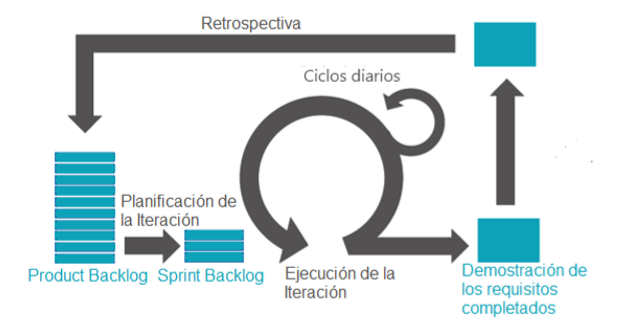
\includegraphics[width=0.95\linewidth]{figuras/ciclo}}
	\caption[Ciclo]{Ciclo del proyecto}
	\label{fig:ciclo}
\end{figure}


\subsection{Particularidades de este proyecto}
\hspace*{2em}En este proyecto la figura del SCRUM MASTER y el equipo técnico recaen sobre una sola persona.  Bajo esta particularidad desaparecen las reuniones técnicas diarias.
La figura del gestor del producto viene dada por un contacto con la empresa cliente. Las reuniones de comienzo del Sprint y final de Sprint se realizan bajo herramientas de videoconferencia, y teamviewer.	\\ 










	\section{Historias de usuario}
\setlength{\parindent}{2em}
Las historias de usuario, son pequeñas descripciones de los requerimientos de un cliente. Su utilización es común cuando se aplica marcos de entornos ágiles como SCRUM. 

Al redactar las historias de usuario se debe tener en cuenta describir el Rol, la funcionalidad y el resultado esperado en una frase corta. Debe venir acompañada de los criterios de aceptación.

Es deseable que las historias de usuario sean escritas por el usuario, en una frase corta. Debe describir el rol desempeñado por el usuario de forma explícita e indicar el beneficio para el área de negocio que representa esta funcionalidad. 

\subsection{Listado de historias de usuario}

\begin{shaded}
	\underline{\textbf{Historia 1:}}
	\begin{flushleft}	
		\textbf{Como:} Cliente.\\
		\textbf{Quiero:} Analizar el know how de la empresa.\\
		\textbf{Para:} Estudiar la mejor forma de adaptar los requisitos a la forma de trabajar de la empresa.\\ 
	\end{flushleft}			
\end{shaded}

\begin{shaded}
	\underline{\textbf{Historia 2:}}
	\begin{flushleft}	
		\textbf{Como:} Cliente.\\
		\textbf{Quiero:} Disponer de un listado de clientes offline.\\
		\textbf{Para:} Tener a disposición los clientes sin necesidad de estar conectado.\\ 
	\end{flushleft}			
\end{shaded}

\begin{shaded}
	\underline{\textbf{Historia 3:}}
	\begin{flushleft}	
		\textbf{Como:} Cliente.\\
		\textbf{Quiero:} Disponer de un listado de productos offline.\\
		\textbf{Para:} Tener a disposición los productos sin necesidad de estar conectado.\\ 
	\end{flushleft}			
\end{shaded}

\clearpage

\begin{shaded}
	\underline{\textbf{Historia 4:}}
	\begin{flushleft}	
		\textbf{Como:} Cliente.\\
		\textbf{Quiero:} Disponer de un listado de pedidos por cliente offline.\\
		\textbf{Para:} Tener a disposición los pedidos realizados por un cliente sin necesidad de estar conectado.\\ 
	\end{flushleft}			
\end{shaded}

\begin{shaded}
	\underline{\textbf{Historia 5:}}
	\begin{flushleft}	
		\textbf{Como:} Cliente.\\
		\textbf{Quiero:} Poder crear pedidos por cliente.\\
		\textbf{Para:} Gestionar en la aplicación los pedidos y tenerlos almacenados.\\ 
	\end{flushleft}			
\end{shaded}

\begin{shaded}
	\underline{\textbf{Historia 6:}}
	\begin{flushleft}	
		\textbf{Como:} Cliente.\\
		\textbf{Quiero:}  Poder editar los pedidos no enviados.\\
		\textbf{Para:} Realizar correcciones antes de enviar los pedidos.\\ 
	\end{flushleft}			
\end{shaded}

\begin{shaded}
	\underline{\textbf{Historia 7:}}
	\begin{flushleft}	
		\textbf{Como:} Cliente.\\
		\textbf{Quiero:} Tener listados de productos por pedido.\\
		\textbf{Para:} Visualizar los productos y gestionar filtros.\\ 
	\end{flushleft}			
\end{shaded}

\begin{shaded}
	\underline{\textbf{Historia 8:}}
	\begin{flushleft}	
		\textbf{Como:} Cliente.\\
		\textbf{Quiero:} Poder enviar los pedidos realizados a la central.\\
		\textbf{Para:} Disponer de una interface que comunique con la la aplicación de gestión.\\ 
	\end{flushleft}			
\end{shaded}

 \clearpage
 
\begin{shaded}
	\underline{\textbf{Historia 9:}}
	\begin{flushleft}	
		\textbf{Como:} Cliente.\\
		\textbf{Quiero:} Completa abstracción de la app vs aplicación de gestión.\\
		\textbf{Para:} No modificar en la medida de lo posible el producto usado hasta ahora, y mantener la forma de trabajar.\\ 
	\end{flushleft}			
\end{shaded} 


\begin{shaded}
	\underline{\textbf{Historia 10:}}
	\begin{flushleft}	
		\textbf{Como:} Cliente.\\
		\textbf{Quiero:} probar la funcionalidad.\\
		\textbf{Para:} tener un tiempo de pruebas para verificar la funcionalidad de la app.\\ 
	\end{flushleft}			
\end{shaded} 

\section{Product Backlog}

Se estima que la realización del proyecto tendrá una estimación de 5 Iteraciones (2 semanas por iteración) para la fase de desarrollo y 1 Iteración adicional para testeo y pruebas finales con el cliente. Se ha concretado con el cliente unas funcionalidades a través de las historias de usuario. Dejando para una fase posterior, fuera de esta planificación y por ende fuera de este proyecto, Modificaciones adicionales o sugerencias por parte del cliente. 

La jornada diaria tendrá un valor de 1 punto correspondiendo este a una jornada laboral de 8h/dia. Así pues una iteración dispondrá de 10 puntos, que equivalen a los 10 dias laborables incluidos en las dos semanas descritas.

\begin{figure}[H]
	\centering
	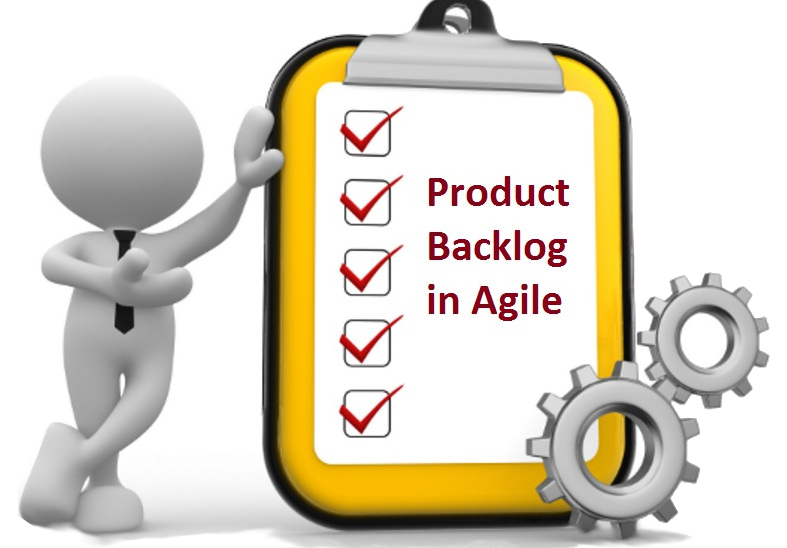
\includegraphics[width=0.55\linewidth]{figuras/spring}
	\label{fig:spring}
\end{figure}

A continuación en la Tabla 4.1 se detalla el Product Backlog inicial, con las historias  de usuario a implementar priorizadas según las necesidades detectadas por el equipo de desarrollo y el Director del proyecto. 

\begin{table}[H]
	\centering
	\caption{Product backlog}
	\label{Product backlog}
	\renewcommand{\arraystretch}{2}
	\begin{tabular}{cccc}
		\multicolumn{4}{c}{\cellcolor{tittletable}{\color{white} \textbf{Product Backlog}}} \\
		\rowcolor{HeaderCol} 
		{\color{white} \textbf{ID}} & {\color{white}  \textbf{Nombre historia}} & {\color{white} \textbf{Estimación}} & {\color{white} \textbf{Prioridad}} \\ 
		\hline
		
		\multicolumn{1}{|c|}{1} & \multicolumn{1}{l|}{Analizar el know how de la empresa} & \multicolumn{1}{c|}{10} & \multicolumn{1}{c|}{Media} \\ \hline
		
		\multicolumn{1}{|c|}{2} & \multicolumn{1}{l|}{Disponer de un listado de clientes offline} & \multicolumn{1}{c|}{5} & \multicolumn{1}{c|}{Media} \\ \hline
	
		\multicolumn{1}{|c|}{3} & \multicolumn{1}{l|}{Disponer de un listado de pedidos por cliente offline} & \multicolumn{1}{c|}{5} & \multicolumn{1}{c|}{Media} \\ \hline
			
		\multicolumn{1}{|c|}{4} & \multicolumn{1}{l|}{Disponer de un listado de productos offline} & \multicolumn{1}{c|}{5} & \multicolumn{1}{c|}{Media} \\ \hline
			
		\multicolumn{1}{|c|}{5} & \multicolumn{1}{l|}{Poder crear pedidos por cliente} & \multicolumn{1}{c|}{8} & \multicolumn{1}{c|}{Alta} \\ \hline
				
		\multicolumn{1}{|c|}{6} & \multicolumn{1}{l|}{Poder editar los pedidos no enviados.} & \multicolumn{1}{c|}{8} & \multicolumn{1}{c|}{Alta} \\ \hline
					
		\multicolumn{1}{|c|}{7} & \multicolumn{1}{l|}{Tener listados de productos por pedido} & \multicolumn{1}{c|}{5} & \multicolumn{1}{c|}{Alta} \\ \hline
						
		\multicolumn{1}{|c|}{8} & \multicolumn{1}{l|}{Poder enviar los pedidos realizados a la central} & \multicolumn{1}{c|}{5} & \multicolumn{1}{c|}{Alta} \\ \hline
		
		\multicolumn{1}{|c|}{9} & \multicolumn{1}{l|}{Completa abstracción de la app vs aplicación de gestión} & \multicolumn{1}{c|}{2} & \multicolumn{1}{c|}{Baja} \\ \hline
		
		\multicolumn{1}{|c|}{10} & \multicolumn{1}{l|}{Probar la funcionalidad} & \multicolumn{1}{c|}{2} & \multicolumn{1}{c|}{Alta} \\ \hline
	\end{tabular}
\end{table}

\clearpage

Más adelante en la Tabla 4.2 se muestra la planificación de las iteraciones con sus respectivas historias y objetivos a cumplir en cada ciclo. 

\begin{table}[H]
	\centering
	\caption{Iteraciones}
	\label{Iteraciones}
	\renewcommand{\arraystretch}{2}
	
	\begin{tabular}{cccccc}
		\multicolumn{6}{c}{\cellcolor{tittletable}{\color{white} \textbf{Iteraciones}}} \\
		\rowcolor{HeaderCol} 
		{\color{white} \textbf{Ite.}} & {\color{white}  \textbf{Inicio}} & {\color{white} \textbf{Fin}} & {\color{white} \textbf{Historias}}  & {\color{white} \textbf{Puntos}} & {\color{white} \textbf{Objetivos}}\\ 
		\hline
		
		\multicolumn{1}{|c|}{1} & \multicolumn{1}{l|}{01/01/2018} 
		& \multicolumn{1}{c|}{12/01/2018} & \multicolumn{1}{c|}{1} 
		& \multicolumn{1}{c|}{10}  & \multicolumn{1}{p{6cm}|}{	
			Analizar como recuperar los datos a procesar.
			Analizar como se insertan los pedidos en la aplicación de gestión existente.
			Ver y plantear la Querys necesarias para operar la DB.
			Iniciar la generación del servicio web que va a comunicar con la BD.
		} \\ \hline
		\multicolumn{1}{|c|}{2} & \multicolumn{1}{l|}{15/01/2018} 
		& \multicolumn{1}{c|}{26/01/2018} & \multicolumn{1}{c|}{2} 
		& \multicolumn{1}{c|}{10}  & \multicolumn{1}{p{5.0cm}|}{
			Desarrollar conjunto para realizar sincronización de datos.	
			Aplicar métodos de consulta al servicio web.
		} \\ \hline
		
		\multicolumn{1}{|c|}{3} & \multicolumn{1}{l|}{29/01/2018} 
		& \multicolumn{1}{c|}{09/02/2018} & \multicolumn{1}{c|}{1.8} 
		& \multicolumn{1}{c|}{10}  & \multicolumn{1}{p{5.0cm}|}{
			Desarrollar conjunto para realizar pedidos.	
			Aplicar métodos de consulta al servicio web.
			Aplicar métodos de inserción al servicio web.
		} \\ \hline
		
		\multicolumn{1}{|c|}{4} & \multicolumn{1}{l|}{12/02/2018} 
		& \multicolumn{1}{c|}{23/02/2018} & \multicolumn{1}{c|}{1.7} 
		& \multicolumn{1}{c|}{10}  & \multicolumn{1}{p{5.0cm}|}{
			Desarrollar conjunto para editar pedidos no enviados.
			Desarrollar conjunto para ver pedidos no previos. 
			Aplicar métodos de consulta al servicio web.
		} \\ \hline
		
		\multicolumn{1}{|c|}{5} & \multicolumn{1}{l|}{26/01/2018} 
		& \multicolumn{1}{c|}{09/03/2018} & \multicolumn{1}{c|}{2.5} 
		& \multicolumn{1}{c|}{10}  & \multicolumn{1}{p{5.0cm}|}{
			Terminar la generación del servicio web. 		
		} \\ \hline
		
		\multicolumn{1}{|c|}{6} & \multicolumn{1}{l|}{12/03/2018} 
		& \multicolumn{1}{c|}{23/03/2018} & \multicolumn{1}{c|}{1} 
		& \multicolumn{1}{c|}{10}  & \multicolumn{1}{p{5.0cm}|}{
			Pruebas de funcionamiento.
		} \\ \hline

	\end{tabular}

\end{table}

\section{Estimación de costes del proyecto}

Teniendo en cuenta los datos anteriores podemos estimar los siguiente recursos de trabajo:
	\begin{itemize}
		\item \textbf{Trabajo total estimado:} 480 horas.
		\item \textbf{Coste pactado:}  6.999 €.
		\item \textbf{Coste hora:} 14,58 € /h.
	\end{itemize}

\subsection{Cálculo de costes del proyecto}

\subsubsection{Recursos de trabajo}

Analista/Programador informático: $ 28.000 \euro / 14p  / 20d  / 8h = 12.5 \euro/h $ 

\subsubsection{Recursos materiales}

Los recursos materiales se consideran cada uno de ellos con un coste por uso de 1,50\euro en concepto de luz y otros gastos que se cobran independientemente del tiempo de uso: $60d \times 1.50\euro= 90\euro$ 

\begin{table}[H]
	\centering
	\caption{Software}
	\label{Software}
	\renewcommand{\arraystretch}{2}
	
	\begin{tabular}{ccc}
		\multicolumn{3}{c}{\cellcolor{tittletable}{\color{white} \textbf{Software}}} \\
		\rowcolor{HeaderCol} 
		{\color{white} \textbf{Concepto}} & {\color{white} \textbf{Coste}} & {\color{white} \textbf{Licencias}}\\ 
		\hline
		
		\multicolumn{1}{|p{6cm}|}{MS Windows 10} & \multicolumn{1}{r|}{149,00\euro} 
		& \multicolumn{1}{c|}{1}\\ \hline
		
		\multicolumn{1}{|p{6cm}|}{Text Studio 2.12} & \multicolumn{1}{r|}{0,00\euro} 
		& \multicolumn{1}{c|}{1}\\ \hline
		
		\multicolumn{1}{|p{6cm}|}{Gimp 2.8} & \multicolumn{1}{r|}{0,00\euro} 
		& \multicolumn{1}{c|}{1}\\ \hline
		
		\multicolumn{1}{|p{6cm}|}{Eclipse oxygen} & \multicolumn{1}{r|}{0,00\euro} 
		& \multicolumn{1}{c|}{1}\\ \hline
		
		\multicolumn{1}{|p{6cm}|}{Android Studio 3.1} & \multicolumn{1}{r|}{0,00\euro} 
		& \multicolumn{1}{c|}{1}\\ \hline
		
	\end{tabular}
	
\end{table}

\subsubsection{Costes totales}
En la siguiente lista se detallan los costes del proyecto. Aunque a priori parezcan que son deficitarios con una desviación de 853\euro en perdidas, hay que tener en cuenta que la figura del analista programador y el gestor del proyecto es la misma y las perdidas son absorbidas por su remuneración.  

\begin{figure}[H]
	\centering
	\begin{tabular}{lr}
		\textbf{Concepto} & \textbf{Coste} \\ \hline \\
		Trabajo & 6.000,00\euro \\
		Materiales	& 240,00\euro \\
		Total & 6.240,00\euro \\
		Gastos(4) & 249,60\euro \\
		Subtotal & 6.489,60\euro \\
		IVA(18)	& 1.362,82\euro \\
		Total & 7852,42\euro \\ \hline
		
	\end{tabular} 
\end{figure}

\section{Seguimiento del Proyecto}

\subsection{1º Iteración}
Durante la primera iteración, se proyecta realizar el análisis correspondiente de la aplicación cliente y sus posibles implicaciones posteriores. La aplicación cliente se encuentra en un servidor centralizado con una base de datos relacional PostgreSQL.
En principio se tiene bastante claro que datos se tienen que recoger y con que formato se insertan los pedidos en la misma. Se desarrollan consultas \textit{(query)} SQL\textsl{} previas para su uso posterior.
\subsubsection{Comentarios y conclusiones }
No hay desviaciones aparentes y se encuentra en plazo.

\subsection{2º Iteración}
En la segunda iteración se trabaja en la gestión de los listados y el esqueleto de las dos aplicaciones, se ha definido la comunicación y la manera de operar de las mismas. 
\subsubsection{Comentarios y conclusiones }
Aparece una ligera desviación que se presupone será incremental en las subsiguientes iteraciones. Hay una pequeña linea difusa entre los diferentes listados que origina la 
creación de código que a priori esta planificado para iteraciones posteriores.
\subsection{3º Iteración}
En la tercera iteración estaba planificado el desarrollo primario de la gestión de pedidos. Durante la creación de las pantallas básicas no se había tenido en cuenta el tiempo de creación de los iconos e imágenes del sistema.
\subsubsection{Comentarios y conclusiones }
El diseño de la apariencia de la aplicación  Android no se había tenido en cuenta, así pues se dedica una parte importante de la iteración a realizar todos los diseños que vamos a necesitar, tanto para esta iteración como para las posteriores. Se espera absorber este tiempo en iteraciones posteriores.
\subsection{4º Iteración}
Se procede al desarrollo de código fuente para gestionar los pedidos al completo
\subsubsection{Comentarios y conclusiones }
La elección de tecnologías de desarrollo ágiles como el proyecto Lombok, o AndroidAnnotations, que simplifican la generación de código, permiten absorber las desviaciones temporales acarreadas por las iteraciones posteriores.
\subsection{5º Iteración}
Se finalizan algunas funcionalidades pendientes y se termina el servicio web para gestionar los datos a enviar/recibir.
\subsubsection{Comentarios y conclusiones }
Como estamos por debajo de la estimación se aprovecha para realizar una instalación previa y algunas pruebas.   
\subsection{6º Iteración}
Durante esta Iteración, se realizan pruebas unitarias, de integración y funcionales con el cliente, identificando ligeros fallos que se corrigen durante la duración de esta iteración.  

\subsection{Final de iteraciones}
Una vez extrapolados los datos obtenidos por el tablón de seguimiento, obtenemos unas gráficas que muestran las desviaciones generadas por los diferentes escollos que se han generado durante el desarrollo de la aplicación 

En la siguiente gráfica podemos ver la desviación por iteración:\\
	
\begin{figure}[H]
	\centering
	\begin{tikzpicture} 
		\begin{axis}[ xlabel=Iteración, ylabel=Puntos] 

			\addplot[color=red,mark=x] coordinates { (1,60) (2,50) (3,40) (4,30) (5,20) (6,10)};

			\addplot[color=blue,mark=x] coordinates { (1,60) (2,52) (3,43) (4,30) (5,18) (6,10)};
	
		\end{axis} 
	\end{tikzpicture}
	\captionof{figure}{Product Burn-Down}
	\label{tikz-1}
\end{figure}

\clearpage

En la siguiente gráfica podemos ver la desviación por Iteraciones/día:\\

\begin{figure}[H]
	\centering
	\begin{tikzpicture} 
		\begin{axis}[ xlabel=Iteración, ylabel=Puntos] 

			\addplot[color=red,mark=x] coordinates { (0,60) (1,59) (2,58) (3,57) (4,56) (5,55)
				(6,54) (7,53) (8,52) (9,51) (10,50) (11,49) (12,48) (13,47) (14,46) (15,45) (16,44) (17,43) (18,42) (19,41) (20,40) (21,39) (22,38) (23,37) (24,36) (25,35)
				(26,34) (27,33) (28,32) (29,31) (30,30) (31,29) (32,28) (33,27) (34,26) (35,25) (36,24) (37,23) (38,22) (39,21) (40,20) (41,19) (42,18) (43,17) (44,16) (45,15)
				(46,14) (47,13) (48,12) (49,11) (50,10) (51,9) (52,8) (53,7) (54,6) (55,5)
				(56,4) (57,3) (58,2) (59,1) (60,0)};
			
			\addplot[color=blue,mark=x] coordinates { (0,60) (1,59) (2,58) (3,57) (4,56) (5,55)
				(6,54) (7,53) (8,52) (9,52) (10,52) (11,51) (12,50) (13,49) (14,48) (15,47) (16,47) (17,47) (18,46) (19,46) (20,46) (21,45) (22,45) (23,45) (24,45) (25,44)
				(26,44) (27,44) (28,43) (29,43) (30,43) (31,42) (32,40) (33,37) (34,35) (35,31) (36,29) (37,27) (38,24) (39,22) (40,20) (41,19) (42,18) (43,16) (44,15) (45,13)
				(46,12) (47,10) (48,10) (49,9) (50,8) (51,7) (52,6) (53,5) (54,4) (55,3)
				(56,2) (57,2) (58,1) (59,1) (60,0)};
			
			\addplot[color=green] coordinates { (10,0) (10,60)};
			\addplot[color=green] coordinates { (20,0) (20,60)};
			\addplot[color=green] coordinates { (30,0) (30,60)};
			\addplot[color=green] coordinates { (40,0) (40,60)};
			\addplot[color=green] coordinates { (50,0) (50,60)};
		\end{axis} 
	\end{tikzpicture}
	\captionof{figure}{Sprints BurnDown}
	\label{tikz-2}
\end{figure}


\part{Tecnologías}
	\chapter{Tecnologías utilizadas}

A continuación se presentarán las tecnologías empleadas que permitieron el desarrollo de la herramienta en cuestión. Primero se listan y explican los lenguajes utilizados para la programación y diseño/desarrollo de interfaces, luego las herramientas que dieron soporte al proceso de desarrollo y por último los  entornos  utilizados. 

\section{Lenguajes utilizados}
Se pueden clasificar según su utilización:

\begin{itemize}
	\item \emph{\textbf{Java:}} La herramienta está desarrollada en mayor parte en este lenguaje, ya previamente conocido por el equipo de desarrollo y además tiene las ventajas de disponer de mucha documentación en la web. Para el desarrollo en este lenguaje se  utiliza  el  jdk  1.8. \cite{java} \\
 	\item \emph{\textbf{Groovy:}} Es un lenguaje de programación orientado a objetos implementado sobre la plataforma Java. Tiene características similares a Python, Ruby, Perl y Smalltalk. Se obtiene mayor nivel de abstracción con este lenguaje. \cite{groovy}
\end{itemize}

\section{Herramientas utilizadas}
A continuación se listan las herramientas utilizadas dentro del proceso de   desarrollo  de  la  herramienta: \\

\begin{itemize}
	\item \emph{\textbf{Git+GitHub:}} Para el control de versiones se utilizó Git, un sistema distribuido de control de versiones. Al ser distribuido,   cada desarrollador cuenta con un “clon” completo del repositorio. Cada uno puede realizar cambios sobre el proyecto, lo que permite ser autónomo y trabajar en cualquier situación. Como repositorio central, se decidió utilizar los servicios de GitHub, una plataforma de desarrollo colaborativo de software para el alojamiento de repositorios de proyectos   utilizando el sistema de control de versiones Git. El código se   almacena de forma pública bajo licencias de código Open   Source.  
	\item \emph{\textbf{Kunagi:}} Entre las necesidades para encarar una metodología ágil inspirada en SCRUM, era necesario una herramienta de   soporte para la gestión del desarrollo ágil sin implicar mayores complejidades técnicas. Como se explicó anteriormente,  Kunagi ofrece la administración integrada de proyectos complementando la metodología SCRUM a través de otras mejores prácticas para cubrir todas las necesidades para la   administración de proyectos. Esta herramienta corre     localmente en la máquina de un integrante del equipo, sobre un  servidor  Apache  Tomcat. 
	\item \emph{\textbf{Gimp:}} Es un programa de edición de imágenes digitales, tanto dibujos como fotografías. Es un programa libre y gratuito. Forma parte del proyecto GNU y está disponible bajo la Licencia pública general de GNU y GNU Lesser General Public License.

\end{itemize}
	
\section{Entornos de desarrollo}	
Los  entornos  de  programación  utilizados  fueron: 

\begin{itemize}
	\item \emph{\textbf{Eclipse:}} Es una plataforma de software compuesto por un conjunto de herramientas de programación de código abierto multi-plataforma para desarrollar lo que el proyecto llama "Aplicaciones de Cliente Enriquecido", opuesto a las aplicaciones "Cliente-liviano" basadas en navegadores. 
	Esta plataforma, típicamente ha sido usada para desarrollar entornos de desarrollo integrados (del inglés IDE), como el IDE de Java llamado Java Development Toolkit (JDT) y el compilador (ECJ) que se entrega como parte de Eclipse (y que son usados también para desarrollar el mismo Eclipse).\cite{eclipse}
 	
 	\item \emph{\textbf{Android Studio:}} Es el entorno de desarrollo integrado oficial para la plataforma Android. Fue anunciado el 16 de mayo de 2013 en la conferencia Google I/O, y reemplazó a Eclipse como el IDE oficial para el desarrollo de aplicaciones para Android. La primera versión estable fue publicada en diciembre de 2014. \cite{astudio}
\end{itemize}

	\begin{wrapfigure}{r}{21cm}	
		\centering
		
\includegraphics[width=0.14\textwidth]{figuras/git}
		
\includegraphics[width=0.13\textwidth]{figuras/groovy}
		
\includegraphics[width=0.09\textwidth]{figuras/java}
		
\includegraphics[width=0.09\textwidth]{figuras/gimp}
		
\includegraphics[width=0.09\textwidth]{figuras/eclipse}
		
\includegraphics[width=0.08\textwidth]{figuras/astudio}	
	\end{wrapfigure}

\clearpage


\section{Últimas consideraciones}
	
A parte de los entornos de programación tomamos en consideración dos herramientas que mejoran sustancialmente la estructura de las aplicaciones.

\begin{itemize}
	\item \emph{\textbf{Lombok project: }} paquete de librerías en java que permiten ignorar ciertas estructuras tediosas (getters, setters, constructores...) que son integradas en tiempo de compilación. \cite{lombok}
	
	\item \emph{\textbf{AndroidAnnotations: }} paquete de librerías en java que facilita el mantenimiento de aplicaciones en Android, dando una estructura más sencilla de gestionar y fácil de mantener.\cite{ann}
	\begin{itemize}
		\item \emph{\textbf{Inyección de dependencias: }} inyecta vistas, extras,  servicios, recursos, ...
		\item \emph{\textbf{Modelo de subprocesamiento simplificado: }} anotar métodos para ejecutarlos en subprocesos.
		\item \emph{\textbf{Enlace de eventos: }} anotar métodos para controlar eventos en vistas, eliminamos las subclases del tipo\textsl{} listener.
		\item \emph{\textbf{Cliente REST: }} Crea una interfaz de cliente, AndroidAnnotations genera la implementación.
		\item \emph{\textbf{Sin Magia: }} Como se generan subclases en tiempo de compilación, se puede comprobar el código para ver cómo funciona.	
	\end{itemize}
\end{itemize}

\part{Fundamentos}
	\chapter{Fundamentos en la creación de aplicaciones}

\section{Fundamentos de la creación de web-services JAVA}

Para la realización de esta sección se ha tomado como referencia técnica el libro: Fundamentos de programación Java. \cite{javaFun} 

\subsection{Definición}

\begin{shaded}
	\begin{flushleft}	
		Un servicio Web\textit{(web-service)} es una colección de protocolos y estándares que sirven para intercambiar datos entre aplicaciones. La interoperatividad se consigue mediante la adopción de estándares abiertos. 
	\end{flushleft}			
\end{shaded}

Estos servicios proporcionan mecanismos de comunicación estándares entre diferentes aplicaciones, que interactúan entre sí para presentar información dinámica al usuario. Para proporcionar interoperatividad y expansibilidad entre estas aplicaciones, y que al mismo tiempo sea posible su combinación para realizar operaciones complejas, es necesaria una arquitectura de referencia estándar. 
\pagebreak

\subsection{Aspectos comunes de los web-services}

Los aspectos técnicos comunes son: 
\begin{itemize}
	\item Los Servicios Web exponen funcionalidad útil a los usuarios Web mediante un protocolo Web estándar. En la mayoría de casos, el protocolo utilizado es \textbf{Simple Object Access Protocol (SOAP)}. 
	
	\item Los Servicios Web proporcionan un modo de describir sus interfaces con suficiente detalle para permitir a un usuario construir una aplicación cliente para comunicarse con ellos. Esta descripción se proporciona generalmente en un documento XML que responde al nombre de documento\textbf{ Servicios web Description Language (WSDL)}. 
	
	\item Los Servicios Web se registran de modo que los potenciales usuarios puedan encontrarlos. Esto se realiza mediante\textbf{ Universal Discovery Description and Integration (UDDI)}. 
\end{itemize}
	
Aunque la idea de la programación modular no es nueva, el éxito de esta tecnología reside en que se basa en estándares conocidos en los que ya se tiene una gran confianza, como el XML. 

\subsection{Características}
Las principales características son:
\begin{itemize}
	
	\item  Aportan interoperatividad entre aplicaciones de software independientemente de sus propiedades o de las plataformas sobre las que se instalen, permitiendo la interoperatividad entre plataformas de distintos fabricantes mediante protocolos estándar. 
	
	\item  Los servicios web fomentan los estándares y protocolos basados en texto, que hacen más fácil acceder a su contenido y entender su funcionamiento. 

	\item  Al apoyarse en HTTP, los servicios web pueden aprovechar los sistemas cortafuegos sin necesidad de cambiar sus reglas de filtrado. La principal razón para usar servicios Web es que se basan en HTTP sobre TCP en el puerto 80. Dado que las organizaciones protegen sus redes mediante cortafuegos (firewalls) que filtran y bloquean gran parte del tráfico de Internet, cierran casi todos los puertos TCP salvo el 80, que es, precisamente, el que usan los navegadores. Los servicios Web se canalizan por este puerto, por la simple razón de que no resultan bloqueados. 
	
	\item  Permiten que servicios y software de diferentes compañías ubicadas en diferentes lugares geográficos puedan ser combinados fácilmente para proveer servicios integrados. 

	\item  Los servicios web son muy prácticos al aportar gran independencia entre la aplicación que usa el servicio web y el propio servicio. De esta forma, los cambios a lo largo del tiempo en uno no deben afectar al otro. Esta flexibilidad será cada vez más importante, dado que la tendencia a construir grandes aplicaciones a partir de componentes distribuidos más pequeños es cada día más acusada. 

\end{itemize}

\subsection{SOAP}
SOAP es el acrónimo de “Simple Object Access Protocol” y es el protocolo que se oculta tras la tecnología que comúnmente denominamos “Web Services” o servicios web. SOAP es un protocolo extraordinariamente complejo pensado para dar soluciones a casi cualquier necesidad en lo que a comunicaciones se refiere, incluyendo aspectos avanzados de seguridad, transaccionalidad, mensajería asegurada y demás. 

\begin{figure}[H]
	\centering
	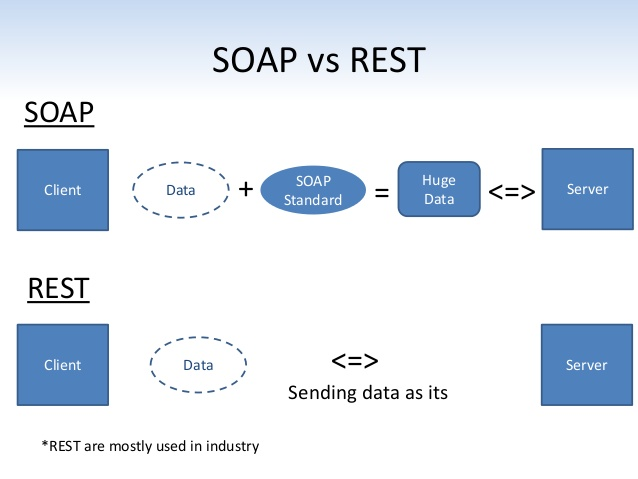
\includegraphics[width=0.7\linewidth]{figuras/soapVSrest}
	\caption{Esquema principal del proyecto Android} 
	\label{fig:soapVSrest}
\end{figure}

\subsection{REST}
REST deriva de \textit{"Representational State Transfer"}, que traducido vendría a ser “transferencia de representación de estado”, más o menos servicio REST no tiene estado \textit{(stateless)}. El estado lo mantiene el cliente y por lo tanto es el cliente quien debe pasar el estado en cada llamada. Si quiero que un servicio REST me recuerde, debo añadirle quien soy en cada llamada. Y lo mismo aplica para el resto de información. 

El no tener estado es una desventaja clara: tener que pasar el estado en cada llamada es, como mínimo, tedioso, pero la contrapartida es clara: esca labilidad. Para mantener un estado se requiere algún sitio (generalmente memoria) donde guardar todos los estados de todos los clientes. A más clientes, más memoria, hasta que al final podemos llegar a no poder admitir más clientes, no por falta de CPU, sino de memoria. 

\subsection{API REST}
En una API REST la idea de “servicio” como tal desaparece. Lo que tenemos son recursos, accesibles por identificadores (URIs). Sobre esos recursos podemos realizar acciones, generalmente diferenciadas a través de verbos HTTP distintos. 

Así, en un servicio web clásico \textbf{(SOAP)} tendríamos un servicio llamado \textbf{\textit{CoffeeService}} que tendría un método \textit{\textbf{GetAll()}} que me devolvería todas los tipos de café. La idea, independientemente de la tecnología usada para consumir el servicio web, es que se llama a un método \textit{\textbf{GetAll()}} de un servicio remoto \textbf{\textit{CoffeeService}}. Del mismo modo para obtener un tipo de café en concreto llamaríamos al método \textit{\textbf{GetById()}} pasándole el id del tipo de café. De ahí que se diga que están orientados a RPC \textit{(Remote Procedure Call – Llamada a método remoto)}. 

Por su parte en un servicio \textbf{(REST)} la propia idea de servicio se desvanece. En su lugar nos queda la idea de un “recurso”, llamémosle “Colección de cafés” que tiene una URI que lo identifica, p. ej. /Coffee. Así, si invoco dicha URI debo obtener una representación de dicho recurso, es decir, debo obtener el listado de todos los tipos de café. 

Para obtener datos de un tipo de café, habrá otro recurso (café) con una URI asociada. Para acceder a uno de sus elementos con una URI tipo /Coffee/123, siendo \textit{123} el ID de la café. 
A la hora de hacer operaciones típicas la URI para acceder es siempre  /Coffee/123 y es el verbo HTTP (GET, POST, PUT, DELETE,...) el que indica cual es la operación que deseamos hacer. 
\begin{figure}[H]
	\centering
	
\includegraphics[width=0.5\linewidth]{figuras/webservice}
	\caption{El conjunto de los Servicios web} 
	\label{fig:webservice}
\end{figure}

\subsection{La elección}
Los servicios web SOAP terminan siendo un monstruo con muchas capacidades pero que en la mayoría de los casos no necesitamos. Por su parte REST es simple. REST no quiere dar soluciones para todo y por lo tanto no pagamos con una demasiada complejidad una potencia que quizá no vamos a necesitar. Así que la elección es clara usaremos REST

\pagebreak


\section{Fundamentos de la creación de aplicaciones Android}

Para la realización de esta sección se ha tomado como referencia técnica el libro: Fundamentos del desarrollo de aplicaciones para Android. \cite{android} 

\subsection{Cómo funciona el sistema operativo Android}
Una vez instalada en un dispositivo, cualquier aplicación corre en su propio entorno limitado de seguridad\cite{android}: 
\begin{itemize}

	\item El sistema operativo Android es un sistema multi-usuario de Linux en el que cada aplicación es un usuario diferente.  

	\item Por defecto, el sistema asigna a cada aplicación de una única ID de usuario \textit{(el ID es utilizado únicamente por el sistema y desconocido para la aplicación)}. Establece permisos para todos los archivos en una aplicación para que sólo el ID asignado pueda acceder a ellos.  

	\item Cada proceso tiene su propia máquina virtual, por lo que el código de una aplicación se ejecuta de forma aislada de otras aplicaciones.  

	\item Por defecto, cada aplicación se ejecuta en su propio proceso de Linux, lo inicia cuando alguno de los componentes se ejecuta, a continuación, cierra el proceso cuando ya no se necesita o cuando el sistema debe recuperar la memoria para otras aplicaciones. 
\end{itemize}

Con esto, el SO implementa \textbf{el principio de privilegios mínimos}, que consiste en que cada aplicación sólo puede acceder a los componentes requeridos para hacer su trabajo. Esto genera un entorno muy seguro en el que la aplicación en cuestión no puede acceder a partes del sistema para las cuales no se le ha otorgado permiso. 
De cualquier modo, existen manera para que una aplicación pueda compartir datos con otras aplicaciones, o también que, una aplicación pueda acceder a los servicios del sistema: 
\begin{itemize}
	
	\item En el caso en el que dos aplicaciones compartan el mismo ID, son capaces de acceder cada una a los archivos de la otra. Para ahorrar recursos del sistema, en este caso en el que dos aplicaciones tienen el mismo ID también se pueden organizar para ejecutar en el mismo proceso de Linux y compartir la misma máquina virtual.  
	
	\item Una aplicación puede solicitar permiso para acceder a los datos del dispositivo, tales como los contactos del usuario, el almacenamiento externo (tarjeta SD), cámara, etc. Todos los permisos de la aplicación debe ser autorizados por el usuario durante la instalación.  
\end{itemize}

\subsection{Componentes de las Aplicaciones Android}

Los principales componentes de toda aplicación Android son:
\begin{itemize}
	 
	\item \emph{\textbf{Actividades\textit{(Activities)}: }} Cada pantalla de una aplicación. Utilizan Vistas (Views) como componentes que muestran información y responden a las acciones del usuario 

	\item \emph{\textbf{Servicios\textit{(Services)}: }} Componentes de la aplicación que se ejecutan deforma invisible, actualizando los datos y las Actividades, y disparando Notificaciones. Realizan el procesamiento normal de la aplicación que debe continuar incluso cuando las Actividades de la aplicación no están visibles. 
	
	\item \emph{\textbf{ Proveedores de Contenidos\textit{(Content Providers)}: }}   Almacenes de datos compartidos. Gestionan las Bases de Datos para las aplicaciones. 

	\item \emph{\textbf{Intenciones\textit{(Intents)}: }} Mecanismo que permite el paso de mensajes destinados a ciertas Actividades o Servicios, o a todo el sistema \textit{( Broadcast Intents)}. Exponen la intención de que se haga algo. 
	
	\item \emph{\textbf{Receptores de Broadcast\textit{(Broadcast Receivers)}: }} Los crean las aplicaciones como consumidores de las Intenciones de broadcast que cumplan ciertos criterios. 

	\item \emph{\textbf{Notificaciones\textit{(Notifications)}: }} Mecanismo que permite a las aplicaciones señalar algo a los usuarios sin interrumpir la Actividad en primer plano. 
\end{itemize}

\begin{figure}[H]
	\centering
	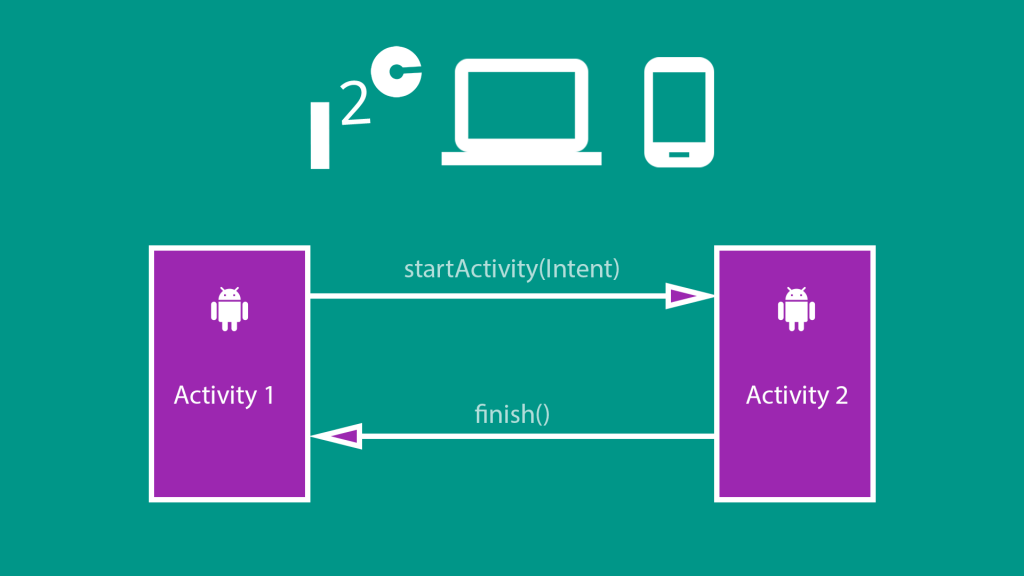
\includegraphics[width=0.8\linewidth]{figuras/activity}
	\caption{Interacción de actividades}
	\label{fig:activity}
\end{figure}



Ademas también existen nuevas implementaciones \textit{(fragmentos, Asíncronos, etc.)} que no vamos a explicar.

\subsection{Manifiesto de una Aplicación Android \textit{(Android manifest)}}

Toda aplicación desarrollada en Android incluye un fichero de Manifiesto, el \textit{\textbf{AndroidManifest.xml}}. Este define la estructura de la aplicación y sus componentes. Incluye un nodo raíz y un nodo para cada uno de sus tipos de componentes. A través de filtros determina como interactuará la aplicacións. 
Algunos de los nodos más importantes son: 
\begin{itemize}
	\item \emph{\textbf{Nodo raíz\textit{(manifest)}: }} Incluye el nombre del paquete de la aplicación. 
	
	\item \emph{\textbf{Nodo aplicación\textit{(application)}: }} Indica los metadatos \textit{(título, icono, tema, etc.)} y contiene los nodos de actividades, servicios, proveedores de contenido y receptores de broadcast. 

	\item \emph{\textbf{Nodo permisos a usar\textit{(uses-permission)}: }}  Declara los permisos necesarios para operar. Estos serán presentados al usuario durante la instalación para que los acepte o deniegue. 

	\item \emph{\textbf{Nodo permisos a proveer\textit{(permission)}: }} Nodo . Define un permiso que se requiere para que otras aplicaciones puedan acceder a partes restringidas de la aplicación. Las otras aplicaciones necesitarán poner un uses-permission en su Manifiesto para utilizar este permiso. 
	
	\item \emph{\textbf{Nodo instrumentación\textit{(instrumentation)}: }} Nodo . Permite definir test de ejecución para las Actividades y Servicios. 
\end{itemize}	

\begin{figure}[H]
	\centering
	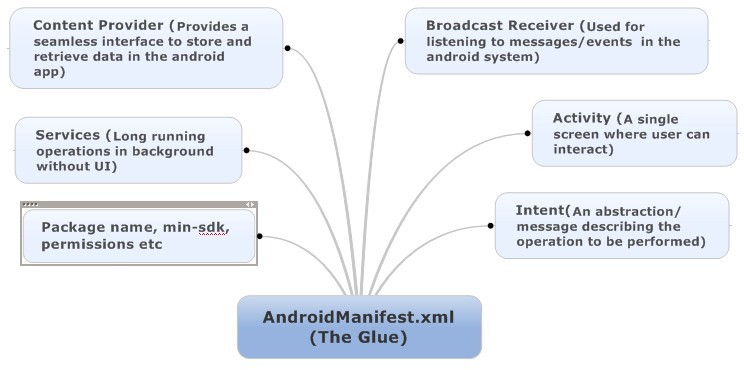
\includegraphics[width=0.95\linewidth]{figuras/androidmanifest}
	\caption{Elementos de un manifiesto Android}
	\label{fig:androidmanifest}
\end{figure}


\subsection{Creación y destrucción de Aplicaciones y Actividades \textit{(Ciclo de vida)}}

Las aplicaciones Android son diferentes a sus homologas en los sistemas operativos tradicionales, en Android sólo hay una aplicación en primer plano que normalmente estará ocupando toda la pantalla. Las aplicaciones estarán formadas por Actividades.
 
Al arrancar una nueva aplicación, pasa a primer plano situando una Actividad encima de la que hubiera, formándose así una pila de actividades. En el momento en el que el usuario presiona el botón “back”, se cierra la actividad en primer plano y recupera la de la cima de la pila. 
Las aplicaciones Android no tienen control ninguno sobre su propio ciclo de vida, esto implica que deben estar pendientes de posibles cambios en su estado y reaccionar como corresponda. En particular deben estar preparadas para su terminación o destrucción en cualquier momento. 
 
Una actividad se puede encontrar en los siguientes estados: 
\begin{itemize}	
	\item \emph{\textbf{Activa\textit{(Running)}: }}  La actividad está encima de la pila, es visible, tiene el foco. Cuando otra actividad pase a estar activa, esta pasará a estar pausada. 
	
	\item \emph{\textbf{Pausada\textit{(Paused)}: }} La actividad es visible pero no tiene el foco. Se alcanza este estado cuando pasa a activa otra actividad transparente o que no ocupa toda la pantalla. Cuando una actividad es tapada por completo pasa a estar parada. 
	
	\item \emph{\textbf{Parada\textit{(Stopped)}: }} Cuando la actividad no es visible. Permanece en memoria reteniendo su estado. Cuando una actividad entra en parada puede ser bueno que salve todos sus datos y el estado de la interfaz de usuario. 

	\item \emph{\textbf{Destruida\textit{(Destroyed)}: }} Cuando la actividad termina, o es matada por el runtime de Android. Sale de la pila de actividades. Necesita ser reiniciada para volver a estar activa. 
\end{itemize}

Y del mismo modo existirán una serie de métodos de transición entre unos estados y otros: 
\begin{itemize}	
	\item \emph{\textbf{onCreate(): }} Se invoca cuando la Actividad se arranca por primera vez. Se utiliza para tareas de inicialización, como crear la interfaz de la Actividad. 
	
	\item \emph{\textbf{onStart(): }} Se invoca cuando la Actividad va a ser mostrada al usuario.
	
	\item \emph{\textbf{onResume(): }} Se invoca cuando la Actividad va a empezar a interactuar con el usuario. 
	
	\item \emph{\textbf{onPause(): }} Se invoca cuando la actividad va a pasar al fondo porque otra actividad ha sido lanzada para ponerse delante. Se utiliza para guardar el estado persistente de la Actividad 
	
	\item \emph{\textbf{onStop(): }} Se invoca cuando la actividad va a dejar de ser visible y no se necesitará durante un tiempo. Si hay escasez de recursos en el sistema, este método podría no llegar a ser invocado y la Actividad ser destruida directamente. 
	
	\item \emph{\textbf{onRestart(): }} Se invoca cuando la Actividad va a salir del estado de parada para volver a estar activa. 
	
	\item \emph{\textbf{onDestroy(): }} Se invoca cuando la Actividad va a ser destruida. Si hay escasez de recursos en el sistema, este método podría no llegar a ser invocado y la Actividad ser destruida directamente. 
  
  	\item \emph{\textbf{onSaveInstanceState(): }} Se invoca para permitir a la actividad guardar su estado, por ejemplo la posición del cursor en una caja de texto. 
  	
 	\item \emph{\textbf{onRestoreInstanceState(): }} Se invoca para recuperar el estado guardado por onSaveInstanceState(). 
\end{itemize}

\begin{figure}[H]
	\centering
	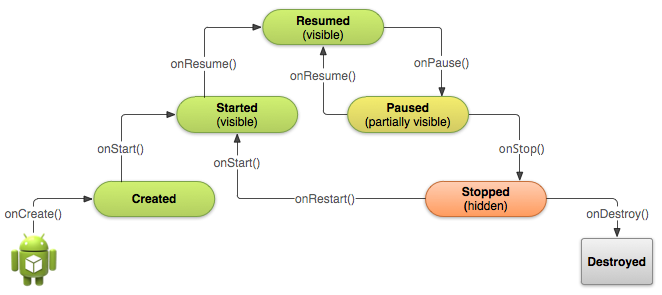
\includegraphics[width=0.95\linewidth]{figuras/estados}
	\caption{Ciclo de una actividad}
	\label{fig:estados}
\end{figure}


\subsection{Recursos de las aplicaciones Android }
 
Una aplicación para Android se compone de algo más que código, requiere de recursos que están separados, como imágenes, archivos de audio, y todo lo relativo a la presentación visual de la aplicación.

Para todos estos recursos Android proporciona un identificador único entero dentro de la aplicación, que puede utilizarse para hacer referencia al recurso en el código de aplicación o de otros recursos definidos en XML. 
Hay distintos tipos de recursos, que se definen en ficheros XML alojados en una cierta subcarpeta de res: 

\begin{itemize}	

	\item \emph{\textbf{Valores simples \textit{(carpeta values)}: }}  Strings, colores y dimensiones. Cada fichero XML contiene la definición de uno o más de estos elementos. Todos estos recursos se identifican con el valor de su atributo name. 
	
	\item \emph{\textbf{Recursos dibujables\textit{(carpeta drawable)}: }} Ficheros con imágenes, incluyendo el icono de la aplicación. Estos recursos se identifican con su nombre de fichero, y los recuadros de color con el valor de su atributo name.
	 
	\item \emph{\textbf{Animaciones\textit{(carpeta anim)}: }} Usados para animaciones sencillas sobre uno o varios gráficos: rotaciones. Fading, movimiento, etc. Cada animación se define en un fichero xML. Se identifican con su nombre de fichero. 
	
	\item \emph{\textbf{menu\textit{(carpeta menu)}: }}  Existen tres tipos de menús: de opciones, contextual y submenú. El menú de opciones y el menú contextual se identifican con su nombre de fichero y el submenú con el valor de su atributo id. 
	
	\item \emph{\textbf{Diseños\textit{(carpeta layout)}: }}  Cada layout se define en un fichero XML. Dentro del layout se definen los elementos que lo componen, como puedan ser los Views o los ViewGroups. Se identificará por su nombre de fichero y los elementos del layout se podrán identificar con su atributo id. 
	
	\item \emph{\textbf{Estilos\textit{(carpeta values)}: }} Un estilo es uno o más atributos que se aplican a un elemento. El tema se define como uno o más atributos que se aplican a todo lo que hay en pantalla, este se asigna como atributo a una actividad en el Manifiesto. El estilo se referencia con el valor de su atributo name.  
					
\end{itemize}

También existen otros recursos como drawables, internacionalización, etc.




	
\part{Estructura}
	\chapter{Diseño Y Estructura}

En este capítulo se describe el diseño final del funcionamiento de la aplicación y se explican los elementos que han influido en las decisiones.


\section{Descripción general}
La solución propuesta, se compone de dos componentes diferenciados , por un lado una aplicación Android y por otro lado un servicio web.

El servicio se comporta como una interface entre la aplicación Android y la plataforma ERP\textsuperscript{\textit{[\ref{glo:erp}]}} que dispone el cliente. A través de la base de datos del ERP el servicio recupera los datos necesarios para proveer a la aplicación Android y también inserta los prepedidos realizados por la misma.

Una de las principales características de la aplicación Android, es que tiene que disponer de los datos necesarios para operar, aunque no dispongamos de conexión en este momento. Para ello dispone de una opción de sincronización de sus datos almacenados con los datos actualizados por la empresa. Para optimizar su rendimiento intentado realizar el menor numero de conexiones, se puede configurar el nº de registros por conexión queremos recuperar.

A efectos de estructurar los datos durante las comunicaciones, la opción elegida es el estándar JSON, que sera explicado mas adelante. 

En la siguiente figura podemos ver un esquema, mostramos de una manera esquemática como es la comunicación entre las partes.

\begin{figure}[H]
	\centering
	\fcolorbox{black}{white}{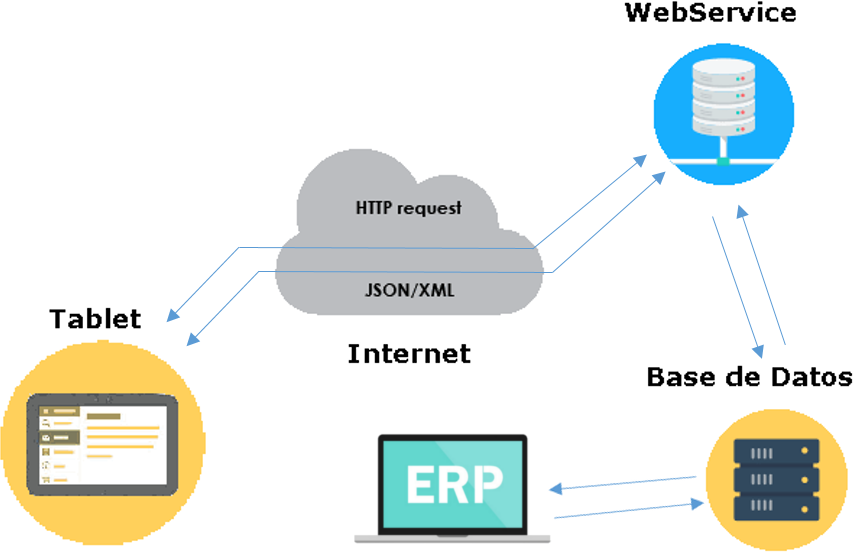
\includegraphics[width=0.9\linewidth]{figuras/esquema}}
	\caption{Esquema principal del proyecto}
	\label{fig:esquema}
\end{figure}


\section{Servicio web}
\subsection{Descripción general}
Antes de abordar la descripción general vamos a definir el termino faceta para su comprensión posterior.
\begin{shaded}
	\begin{flushleft}
	Una faceta, es un aspecto configurable para ejecutar una determinada tarea, cumplir determinados requisitos o tener determinadas características. Por ejemplo, la faceta \textbf{EAR} configura un proyecto para que funcione como una aplicación de empresa añadiendo un descriptor de despliegue y configurando la \textbf{classpath} del proyecto. 
	\end{flushleft}			
\end{shaded}
Dicho esto, dentro del entorno elegido \textit{(Eclipse Oxygen)} hemos elegido un tipo de proyecto \textbf{Dynamic Web Project} que implementa de serie una colección de facetas que serán de ayuda a la hora de desarrollar el servicio web.

\begin{itemize}
	
	\item \emph{\textbf{Dynamic Web Module 3.0: }} Añade soporte para la generación de contenido web dinámico en el API de Servilleta Java.
	\item \emph{\textbf{Java 1.8: }} Añade soporte para la escritura de aplicaciones en  Java.
	\item \emph{\textbf{JavaScript 1.0: }} Permite el desarrollo de Suscriptor utilizando múltiples archivos de origen en una ruta de inclusión configurable.
	\item \emph{\textbf{JAX-RS (REST Web Services) 2.0: }} Permite que el proyecto se implemente con las capacidades de \textbf{JAX-RS}.
\end{itemize}
\subsection{Metodología empleada}
Como hemos comentado en apartados anteriores la elección del tipo de especificación ha sido \textbf{REST}. Al usar esta especificación debemos cumplir con una estructura definida, extbf{JAX-RS}.
\subsubsection{JAX-RS}
Es una \textbf{API} del lenguaje de programación Java que proporciona soporte en la creación de servicios web de acuerdo con el estilo arquitectónico \textbf{REST \textit{(Representational State Transfer)}}. \textbf{JAX-RS} usa anotaciones, introducidas en Java SE 5, para simplificar el desarrollo y despliegue de los clientes y puntos finales de los servicios web.\cite{jaxrs}

\subsection{Diseño e implementación}
Una vez configurado el tipo de proyecto en Eclipse, elegimos \textbf{MAVEN} \textsuperscript{\textit{[\ref{glo:maven}]}} como su constructor de proyectos.

Durante el desarrollo usaremos anotaciones \textsuperscript{\textit{[\ref{glo:anota}]}}, que nos proporciona por defecto \textbf{JAX-RS}, esto nos permite relacionar las URIS del servicio web con el código fuente de una manera mas intuitiva. 

En el ejemplo siguiente mostramos el código fuente correspondiente a la URI : \textit{http://[servidor:puerto]/[servicio]/sincroniza/totales }.\\


\begin{lstlisting}[style=JAVA]
	@Path(value = "/sincroniza")
	public class InTrazaWS {
		
		@GET
		@Path("totales")
		@Produces(MediaType.APPLICATION_JSON)
		public Totales consultaTotalesBD() { 
			return JDBCQuery.getRegistrosTotales(); }	
		.......		
	}
\end{lstlisting}

Vamos a disponer de varias etiquetas de anotación que nos van a proveer de los métodos necesarios para la comunicación con el servicio.

\begin{lstlisting}

@GET - doGet del Servlet
@POST - doPost del Servlet
@Path("prepedido") - path final de la uri
@Consumes(MediaType.APPLICATION\_JSON) consulta por JSON
@Produces(MediaType.APPLICATION\_JSON) escritura por JSON 

\end{lstlisting}

Debemos de definir las rutas para recuperar/insertar los diferentes conjuntos de datos con los que trabajará la aplicación Android. A continuación mostramos un listado de los mismos:\\

\begin{itemize}	
	\item \textbf{totales: } consultaTotalesBD 
	\item \textbf{artículos: } consultaArticulosBD 
	\item \textbf{clientes: } consultaClientesBD 
	\item \textbf{ruteros total fraccionados: } getRuterosTotalFraccionados 
	\item \textbf{rutero tarifa cliente: } consultaTarifaClienteRuteroBD 
	\item \textbf{rutero peso total anio: } consultaPesoTotalAnioRuteroBD 
	\item \textbf{rutero datos: } consultaDatosParaRuteroBD
	\item \textbf{pre-pedido: } enviaPrepedidoBD	\\	
\end{itemize}
 
Cada elemento del listado corresponde a un objeto o conjunto de objetos que se ha procesado de una cadena de caracteres estructurada bajo la especificación \textbf{JSON}. 

Tanto para insertar como para obtener los elementos, se realizaran a través de los métodos del listado, que implementan toda la lógica de operación de la base de datos del cliente, a través del conector java correspondiente. En este caso \textbf{Postgre SQL}.

\subsection{Diagramas}

En la siguiente figura vemos el diagrama \textbf{UML} con las clases principales del servicio web, los accesos a través de intrazaWs y su relación esquemática.\\

\begin{figure}[H]
	\centering
	\fcolorbox{black}{white}{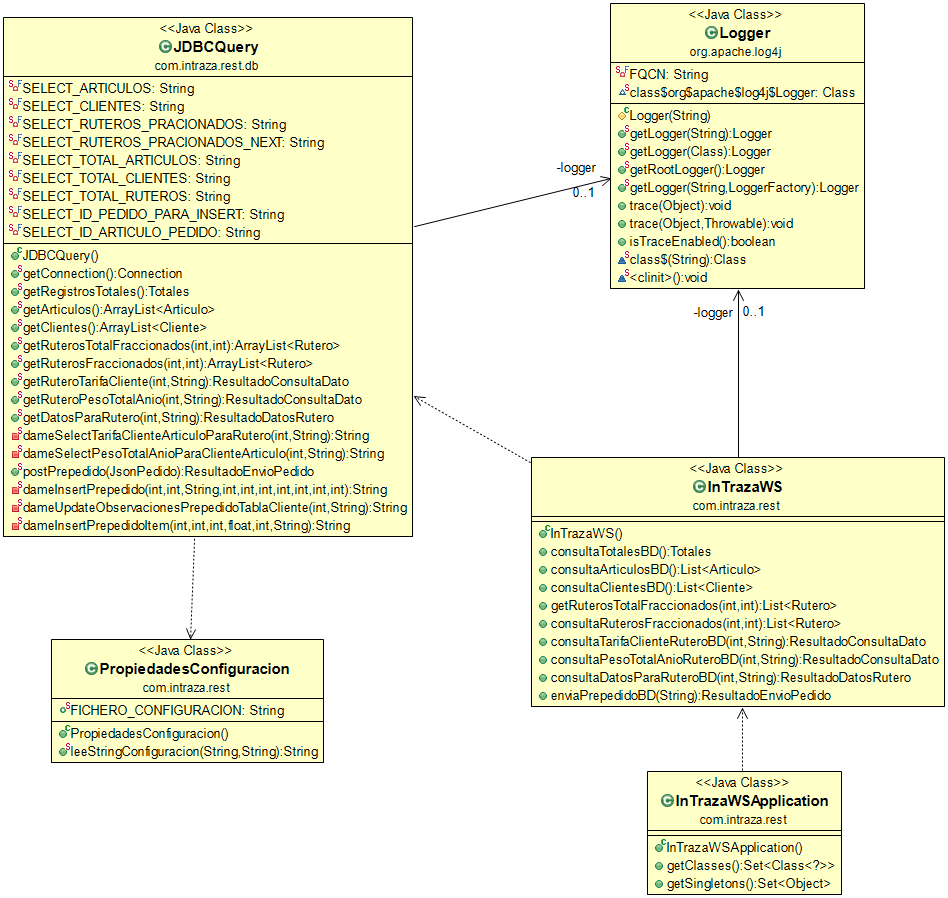
\includegraphics[width=0.58\linewidth]{figuras/dia-web-ser-gen}}
	\caption{Esquema principal del proyecto}
	\label{fig:dia-web-ser-gen}
\end{figure}

\pagebreak

En la siguiente figura vemos el diagrama \textbf{UML} con las relaciones de los objetos transformables a partir de la cadena recibida con la especificación \textbf{JSON}.\\

\begin{figure}[H]
	\centering
	\fcolorbox{black}{white}{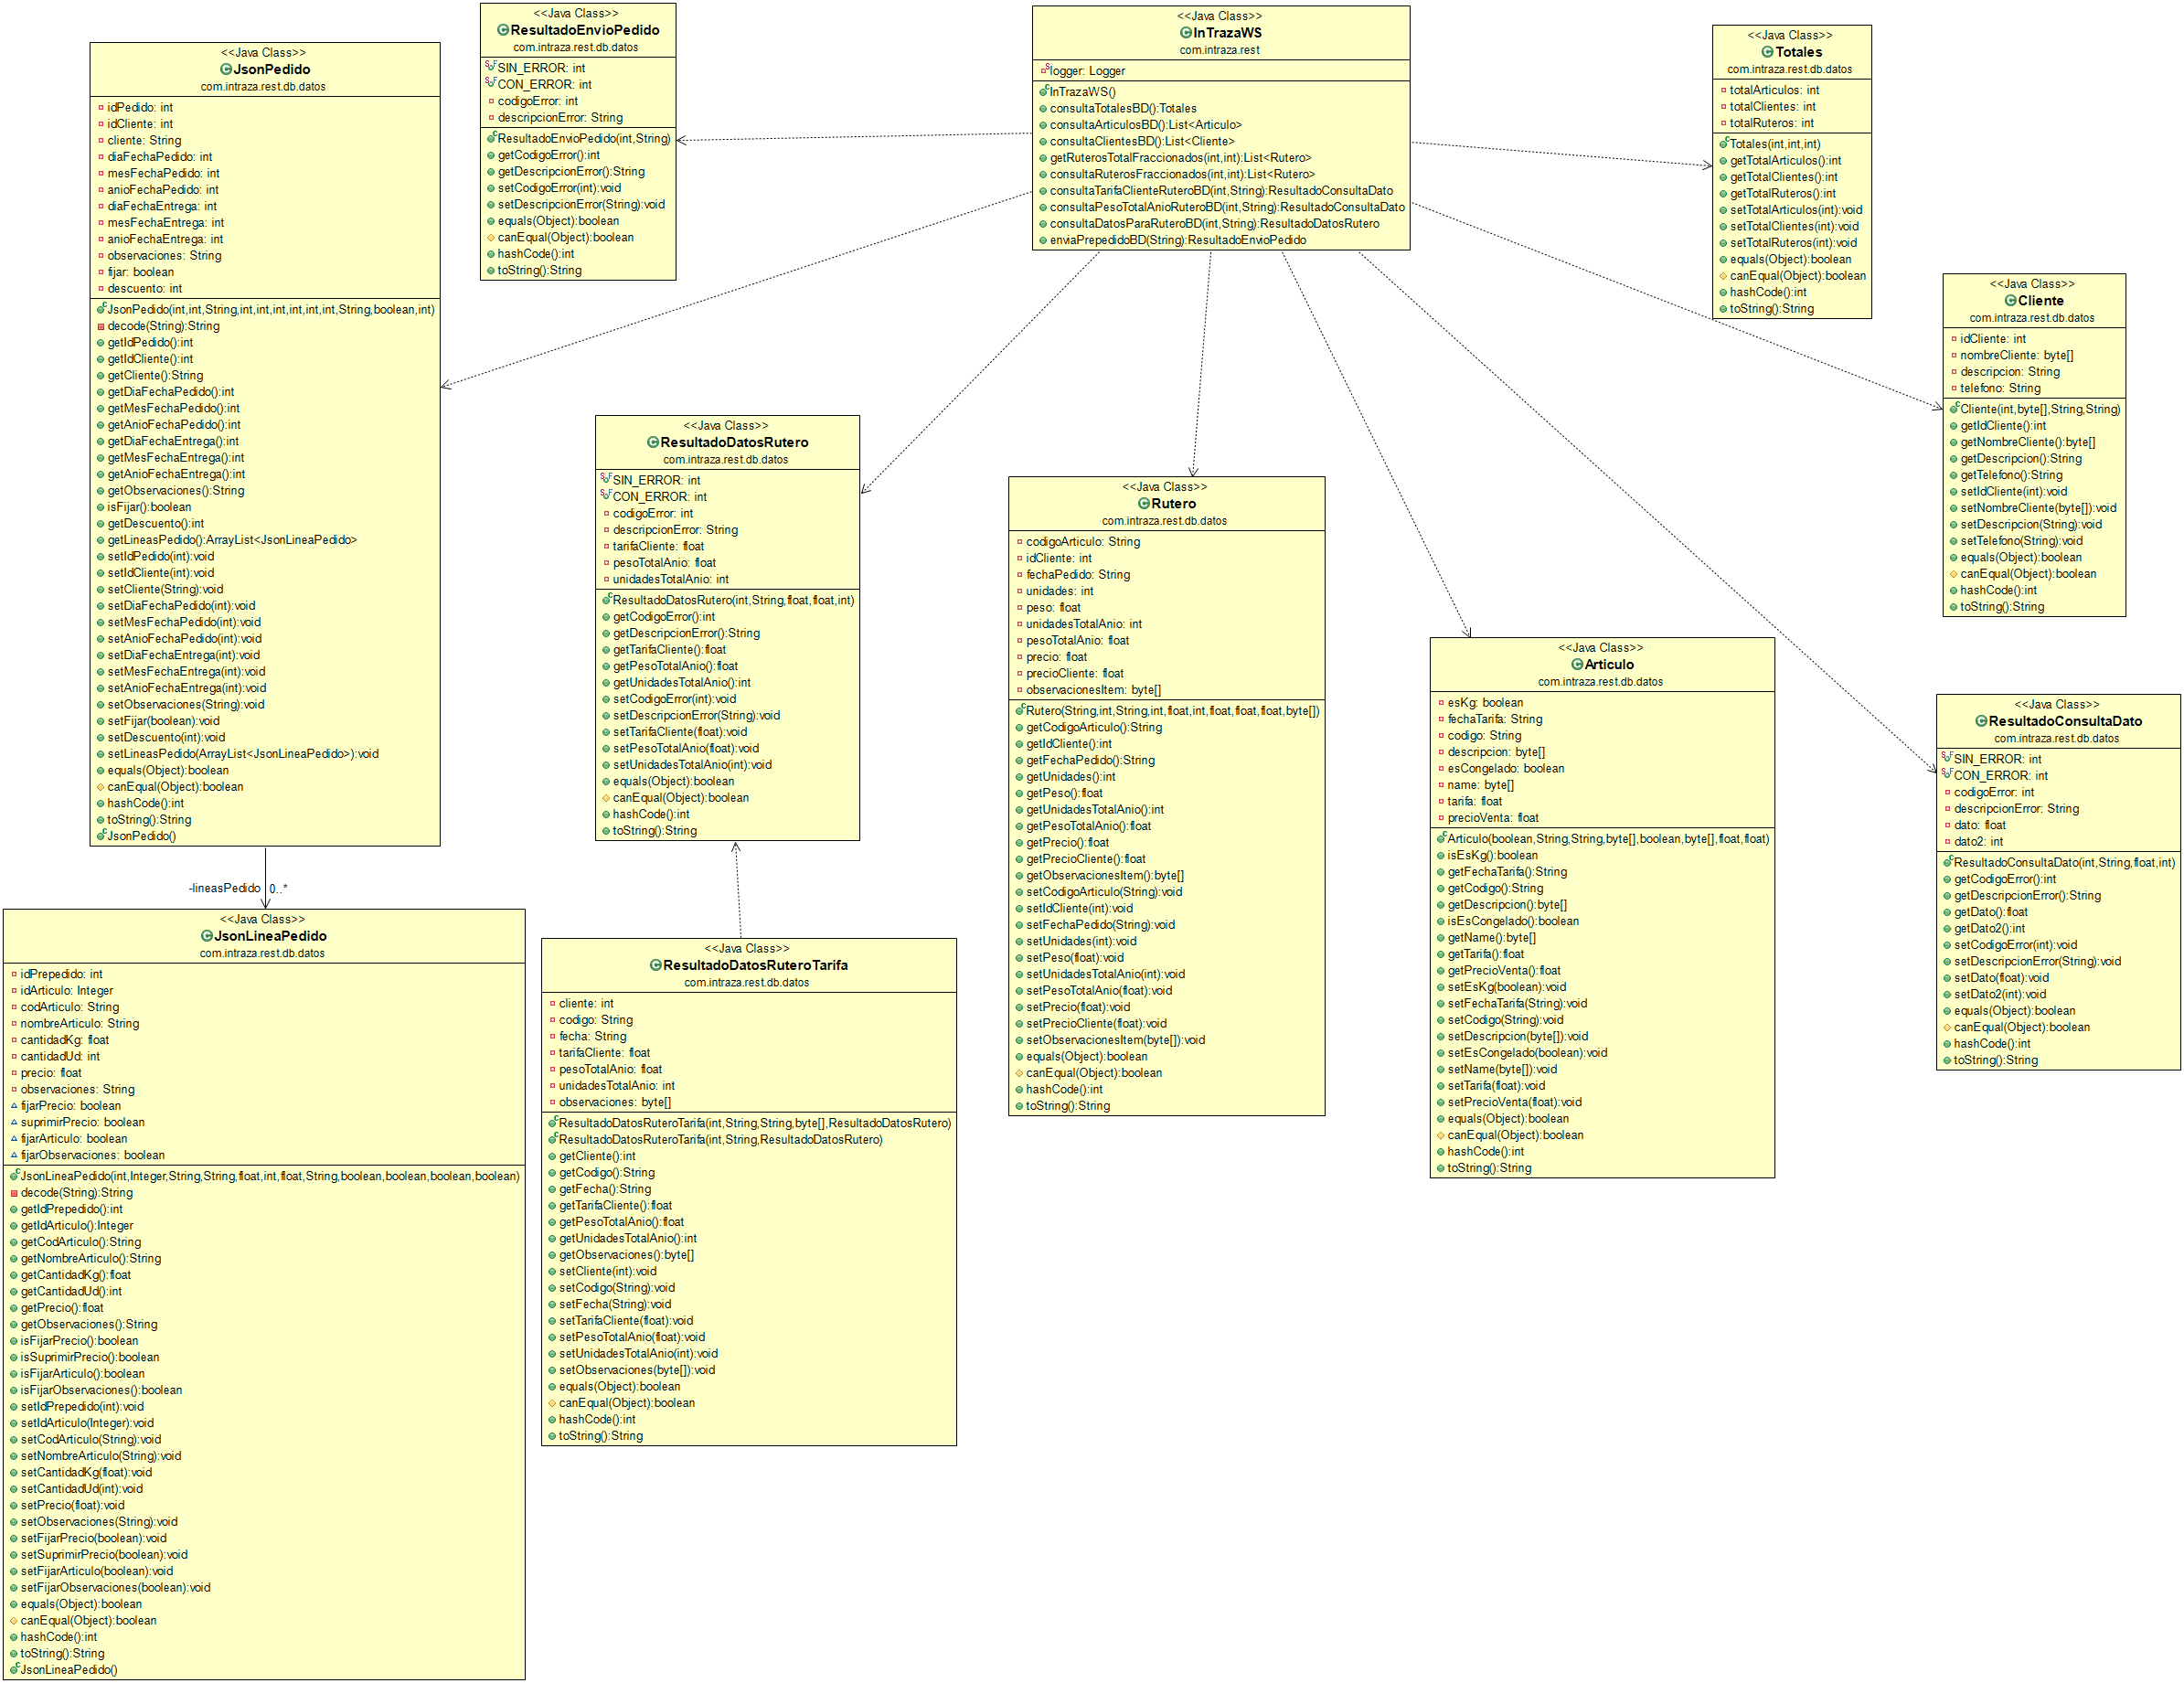
\includegraphics[width=0.9\linewidth,angle=270]{figuras/dia-web-ser}}
	\caption{Relaciones de datos}
	\label{fig:dia-web-ser}
\end{figure}

\pagebreak

En la siguiente figura vemos el diagrama \textbf{UML} con la relación de la clase que gestiona la comunicación con la Base de datos y las clases objeto del servicio.\\

\begin{figure}[H]
	\centering
	\fcolorbox{black}{white}{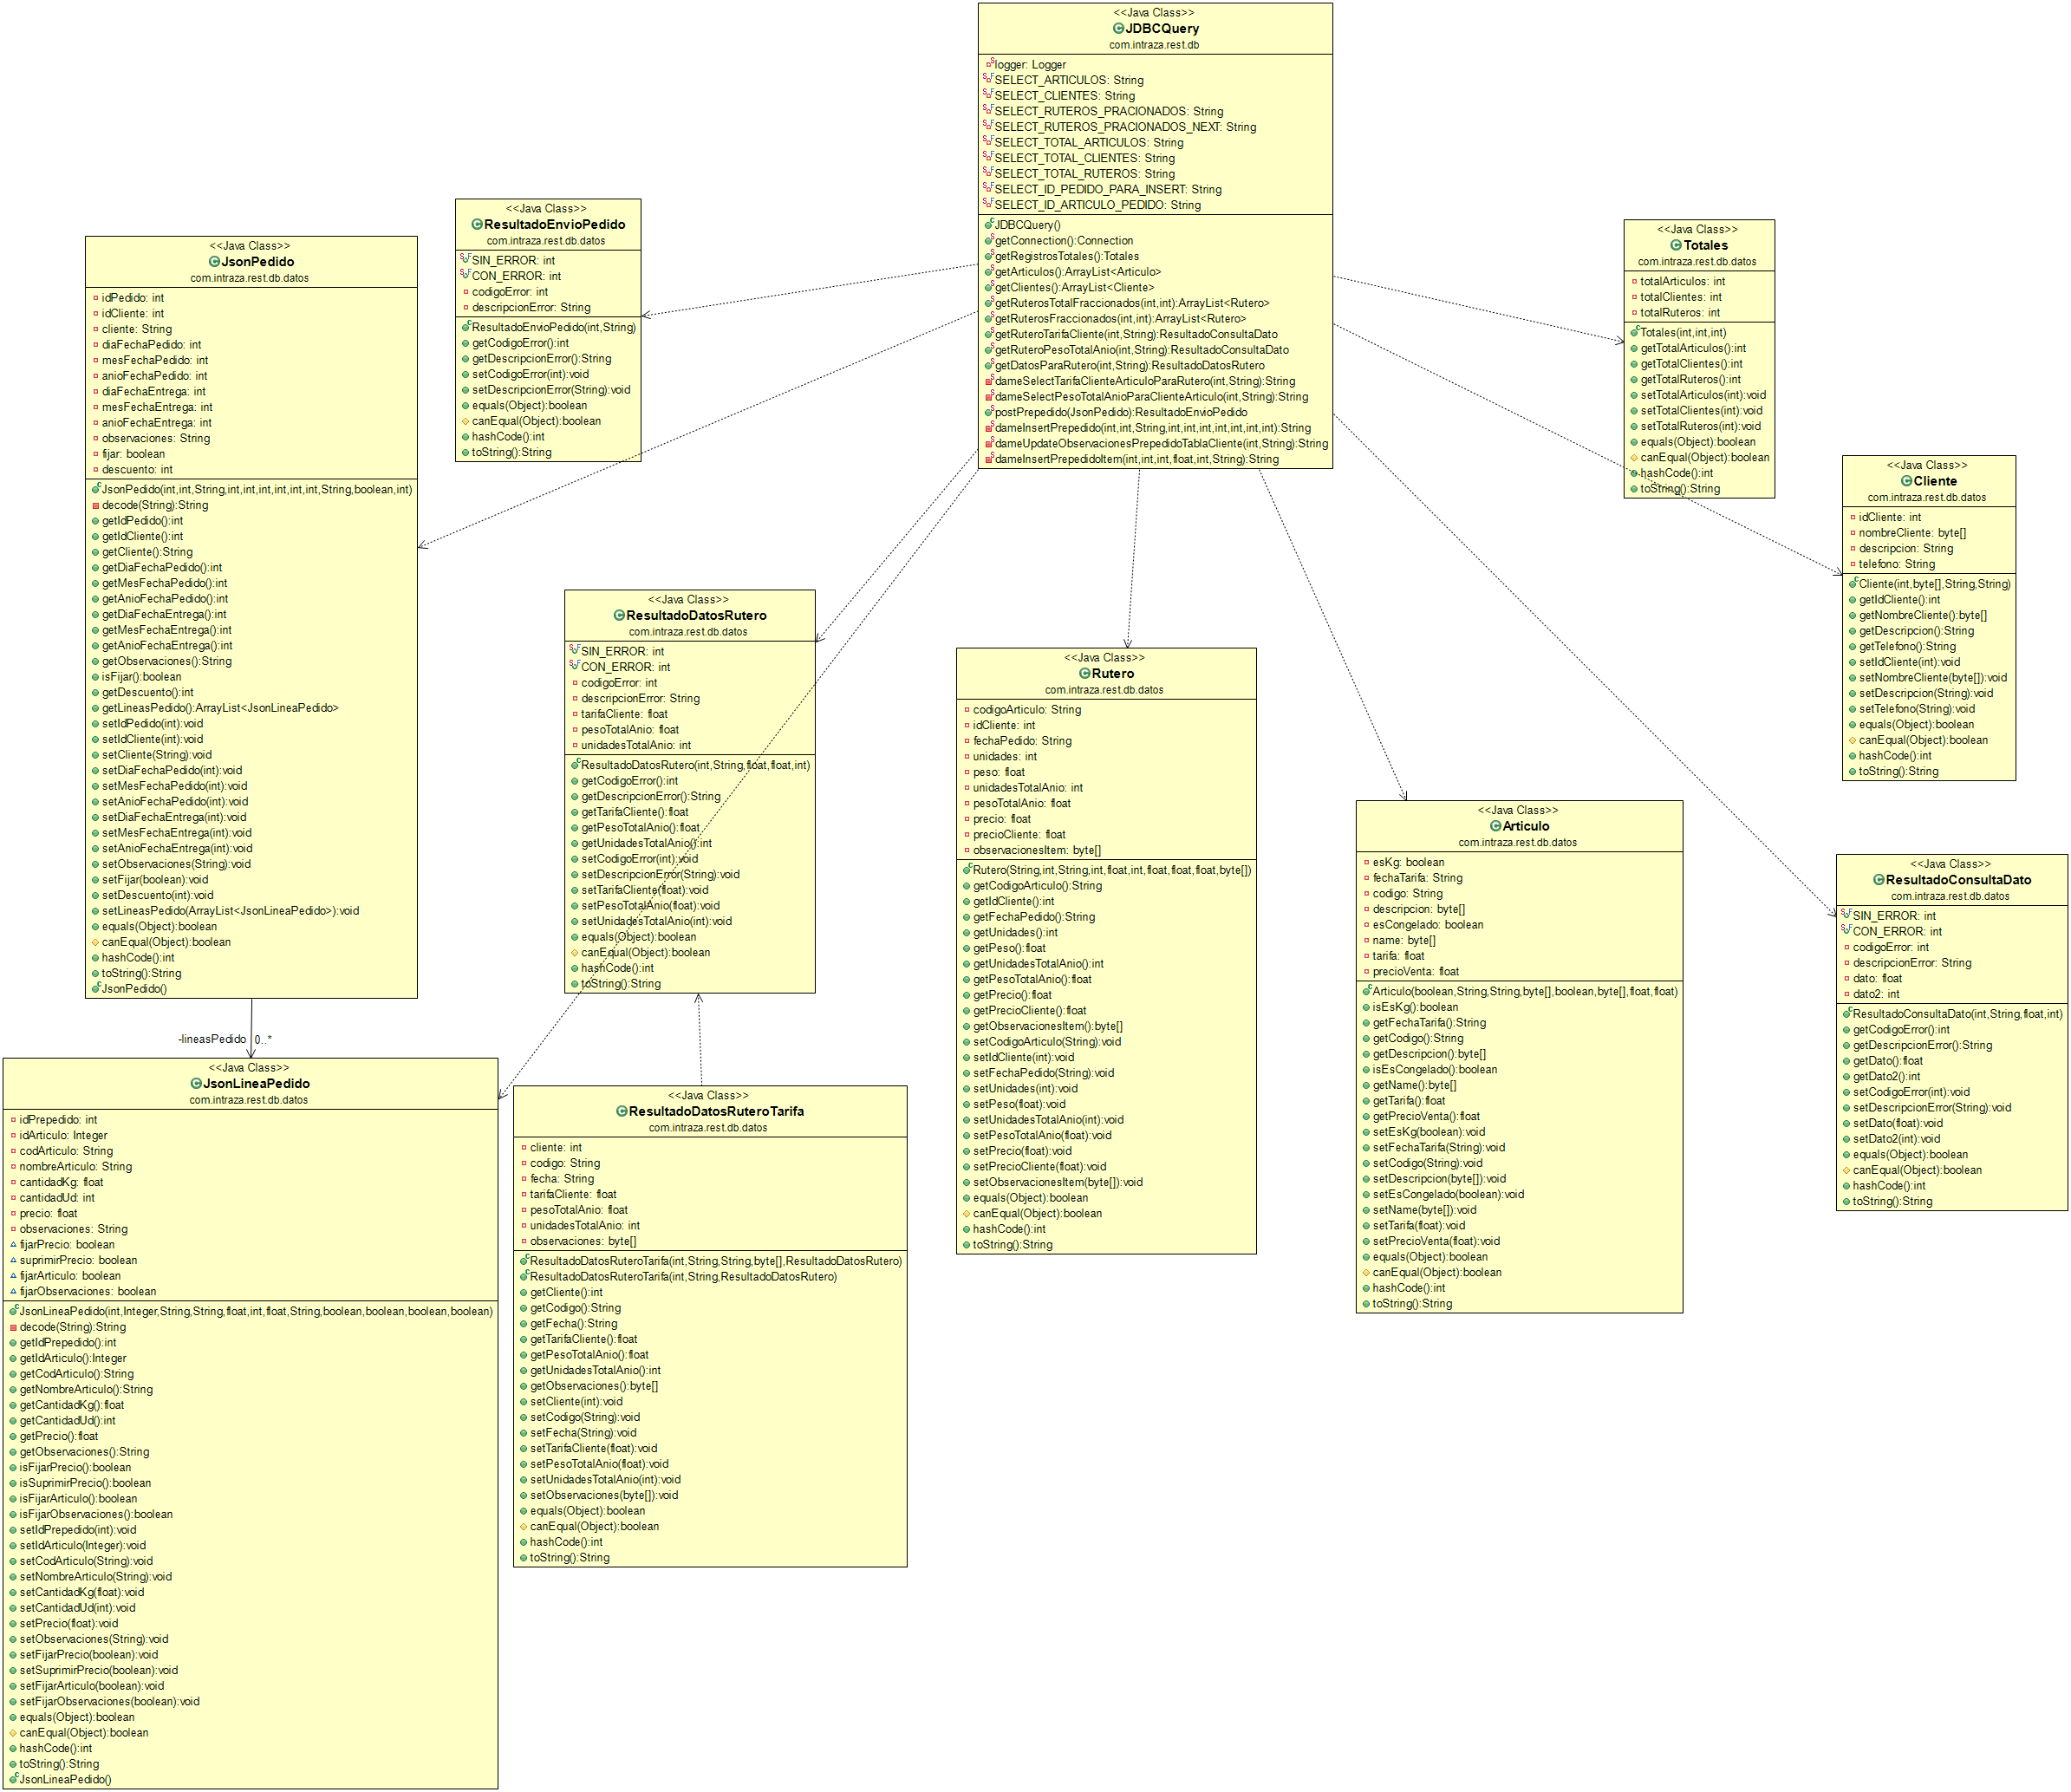
\includegraphics[width=0.9\linewidth,angle=270]{figuras/dia-web-ser-dos}}
	\caption{Relaciones JSON}
	\label{fig:dia-web-ser-dos}
\end{figure}

\pagebreak

\section{Aplicación Android}

\subsection{Descripción general}

Para el desarrollo de la aplicación Android, se ha optado por un programa nativo, usando la herramienta de desarrollo Android studio. Se ha decidido hacerla retro-compatible hasta versión 5, asegurándonos un 80\% de compatibilidad con los terminales del mercado. Como su estructura tópica ya ha sido comentada en capitulo de fundamentos, no vamos a repetir en esta sección lo ya comentado.

\begin{figure}[H]
	\centering
	
\includegraphics[width=0.7\linewidth]{figuras/app}
	\caption{Aplicaciones Android} 
	\label{fig:app}
\end{figure}

La aplicación es un interface de usuario para la gestión de pedidos mientras se encuentra desplazado, pudiendo disponer de datos de gestión de los mismos aunque no pueda establecer comunicación con el servidor. Para ello ademas de las pantallas de operación, dispondrá de una pequeña base de datos (\textbf{SQLlite}) para almacenar los datos de operación.

\subsection{Metodología empleada}

Así como el servicio disponía de \textbf{MAVEN} \textsuperscript{\textit{[\ref{glo:maven}]}} como su constructor de proyectos, en Android studio tendremos \textbf{GRADLE} \textsuperscript{\textit{[\ref{glo:gradle}]}}.

Ademas del SDK de Android dispondremos de las siguientes librerías para poder gestionar todas las necesidades operativas de la aplicación.

\begin{itemize}	
	\item \textbf{Jackson-core: } librería para la gestión de objetos JSON. 
	\item \textbf{Jackson-databind: }  librería para la gestión de objetos JSON. 
	\item \textbf{Lombok: } librería anteriormente comentada. 
	\item \textbf{Androidannotations: } librería anteriormente comentada. 
\end{itemize}

\subsection{Diseño e implementación}
Una vez tenemos la estructura de la aplicación definida, dividiremos la estructura en una actividad principal y 4 actividades secundarias para la gestión de las secciones correspondientes y por último un conjunto de clases \textit{\textbf{Dialog}} para la gestión de ventanas emergentes durante la ejecución

El almacenamiento de datos internos se realiza a través de una base de datos en SQLlite y se definen las siguientes tablas:


\begin{itemize}	
	\item TablaObservacion.
	\item TablaRutero.
	\item TablaPrepedidoItem.
	\item TablaPrepedido.
	\item TablaCliente.
	\item TablaConfiguracion.
\end{itemize}	

Para la gestión de la internacionalización\textit{(I18N)} se definen 4 archivos con los idiomas correspondientes: Castellano, Catalán, Francés, Ingles. 

Se realiza el diseño gráfico de botones, backgrounds, etc, por medio del programa Gimp, y se generan drawables para los efectos visuales del pulsado de botones.

En el ejemplo siguiente mostramos parte del código fuente correspondiente a la actividad principal de la aplicación, se puede comprobar que con las anotaciones realizadas manejamos recursos,eventos,etc, transformando la clase a un formato mas amigable.

\pagebreak

\begin{lstlisting}[style=JAVA]

@EActivity(layout.main)
public class InTrazaActivity extends Activity {
	.......	

	@AfterViews
	void init() {
		config = Configuracion.getInstance();
		config.preparaPropiedades(this);
	}	
	.......	
	
	@OnActivityResult(DIALOGO_PIDE_DATOS_NUEVO_PEDIDO)
	void onResultUno(final int resultCode, final Intent data) {
		if (Activity.RESULT_OK == resultCode) {
			final DatosPedido datosPedido = data.getParcelableExtra("DATOS_PEDIDO");
			pantallaRutero(datosPedido);
		}
		habilitaClickEnActivity(true);
	}
	.......		
}
\end{lstlisting}

Aquí vemos si lo hubiésemos escrito en el formato original java.\\


\begin{lstlisting}[style=JAVA]

public final class InTrazaActivity extends InTrazaActivity implements HasViews, OnViewChangedListener {

	private final OnViewChangedNotifier onViewChangedNotifier_ = new OnViewChangedNotifier();

	final static String DATOS_PEDIDO_EXTRA = "DATOS_PEDIDO";

	@Override
	public void onCreate(Bundle savedInstanceState) {
		OnViewChangedNotifier previousNotifier = OnViewChangedNotifier.replaceNotifier(onViewChangedNotifier);
		init(savedInstanceState);
		super.onCreate(savedInstanceState);
		OnViewChangedNotifier.replaceNotifier(previousNotifier);
		setContentView(R.layout.main);
	}

	@Override
	public<T extends View> T internalFindViewById(int id) {
		return ((T) this.findViewById(id));
	}

	private void init_(Bundle savedInstanceState) {
		Resources resources_ = this.getResources();
		..........
		OnViewChangedNotifier.registerOnViewChangedListener(this);
		..........
		injectExtras();
	}
		..........
}
\end{lstlisting}


\pagebreak

\subsection{Diagramas}
A continuación mostramos los diferentes esquemas, tanto de la base de datos como de las clases de la aplicación Android.

\begin{figure}[H]
	\centering
	\fcolorbox{black}{white}{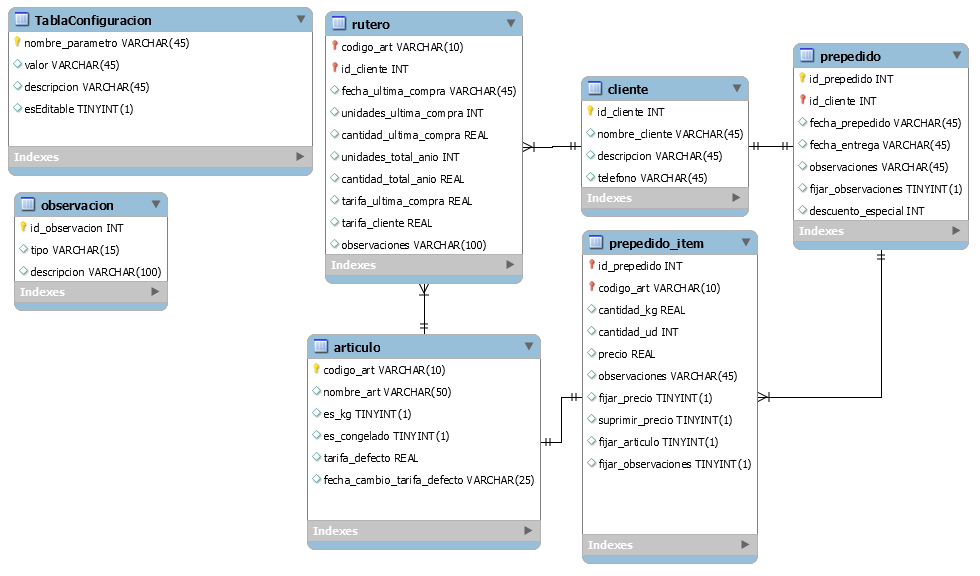
\includegraphics[width=0.6\linewidth]{figuras/eSQLlite}}
	\caption{Esquema de la base de datos SQLlite}
	\label{fig:eSQLlite}
\end{figure}

\begin{figure}[H]
	\centering
	\fcolorbox{black}{white}{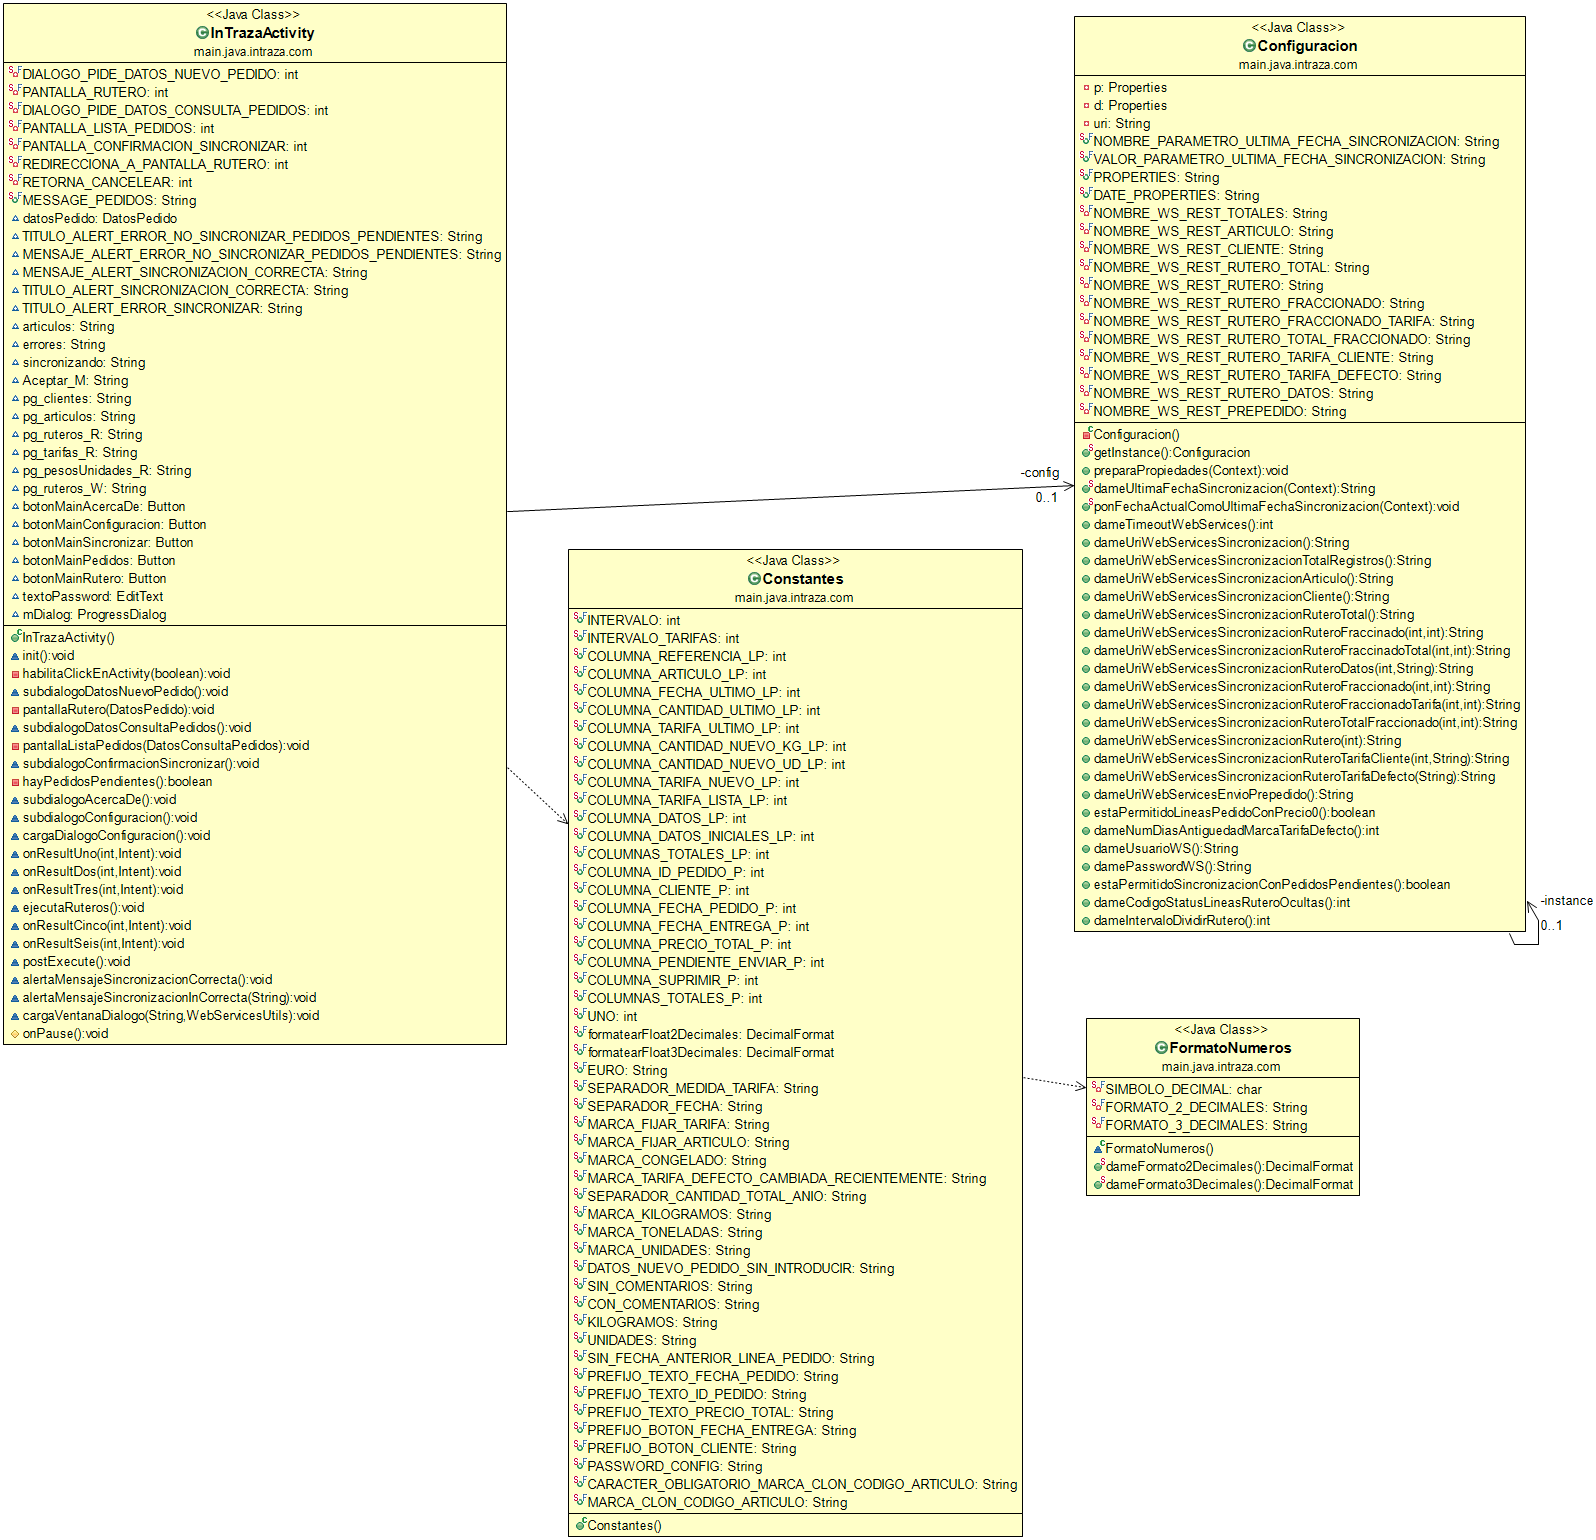
\includegraphics[width=0.6\linewidth]{figuras/and-general}}
	\caption{Esquema principal del proyecto Android} 
	\label{fig:and-general}
\end{figure}

\begin{figure}[H]
	\centering
	\fcolorbox{black}{white}{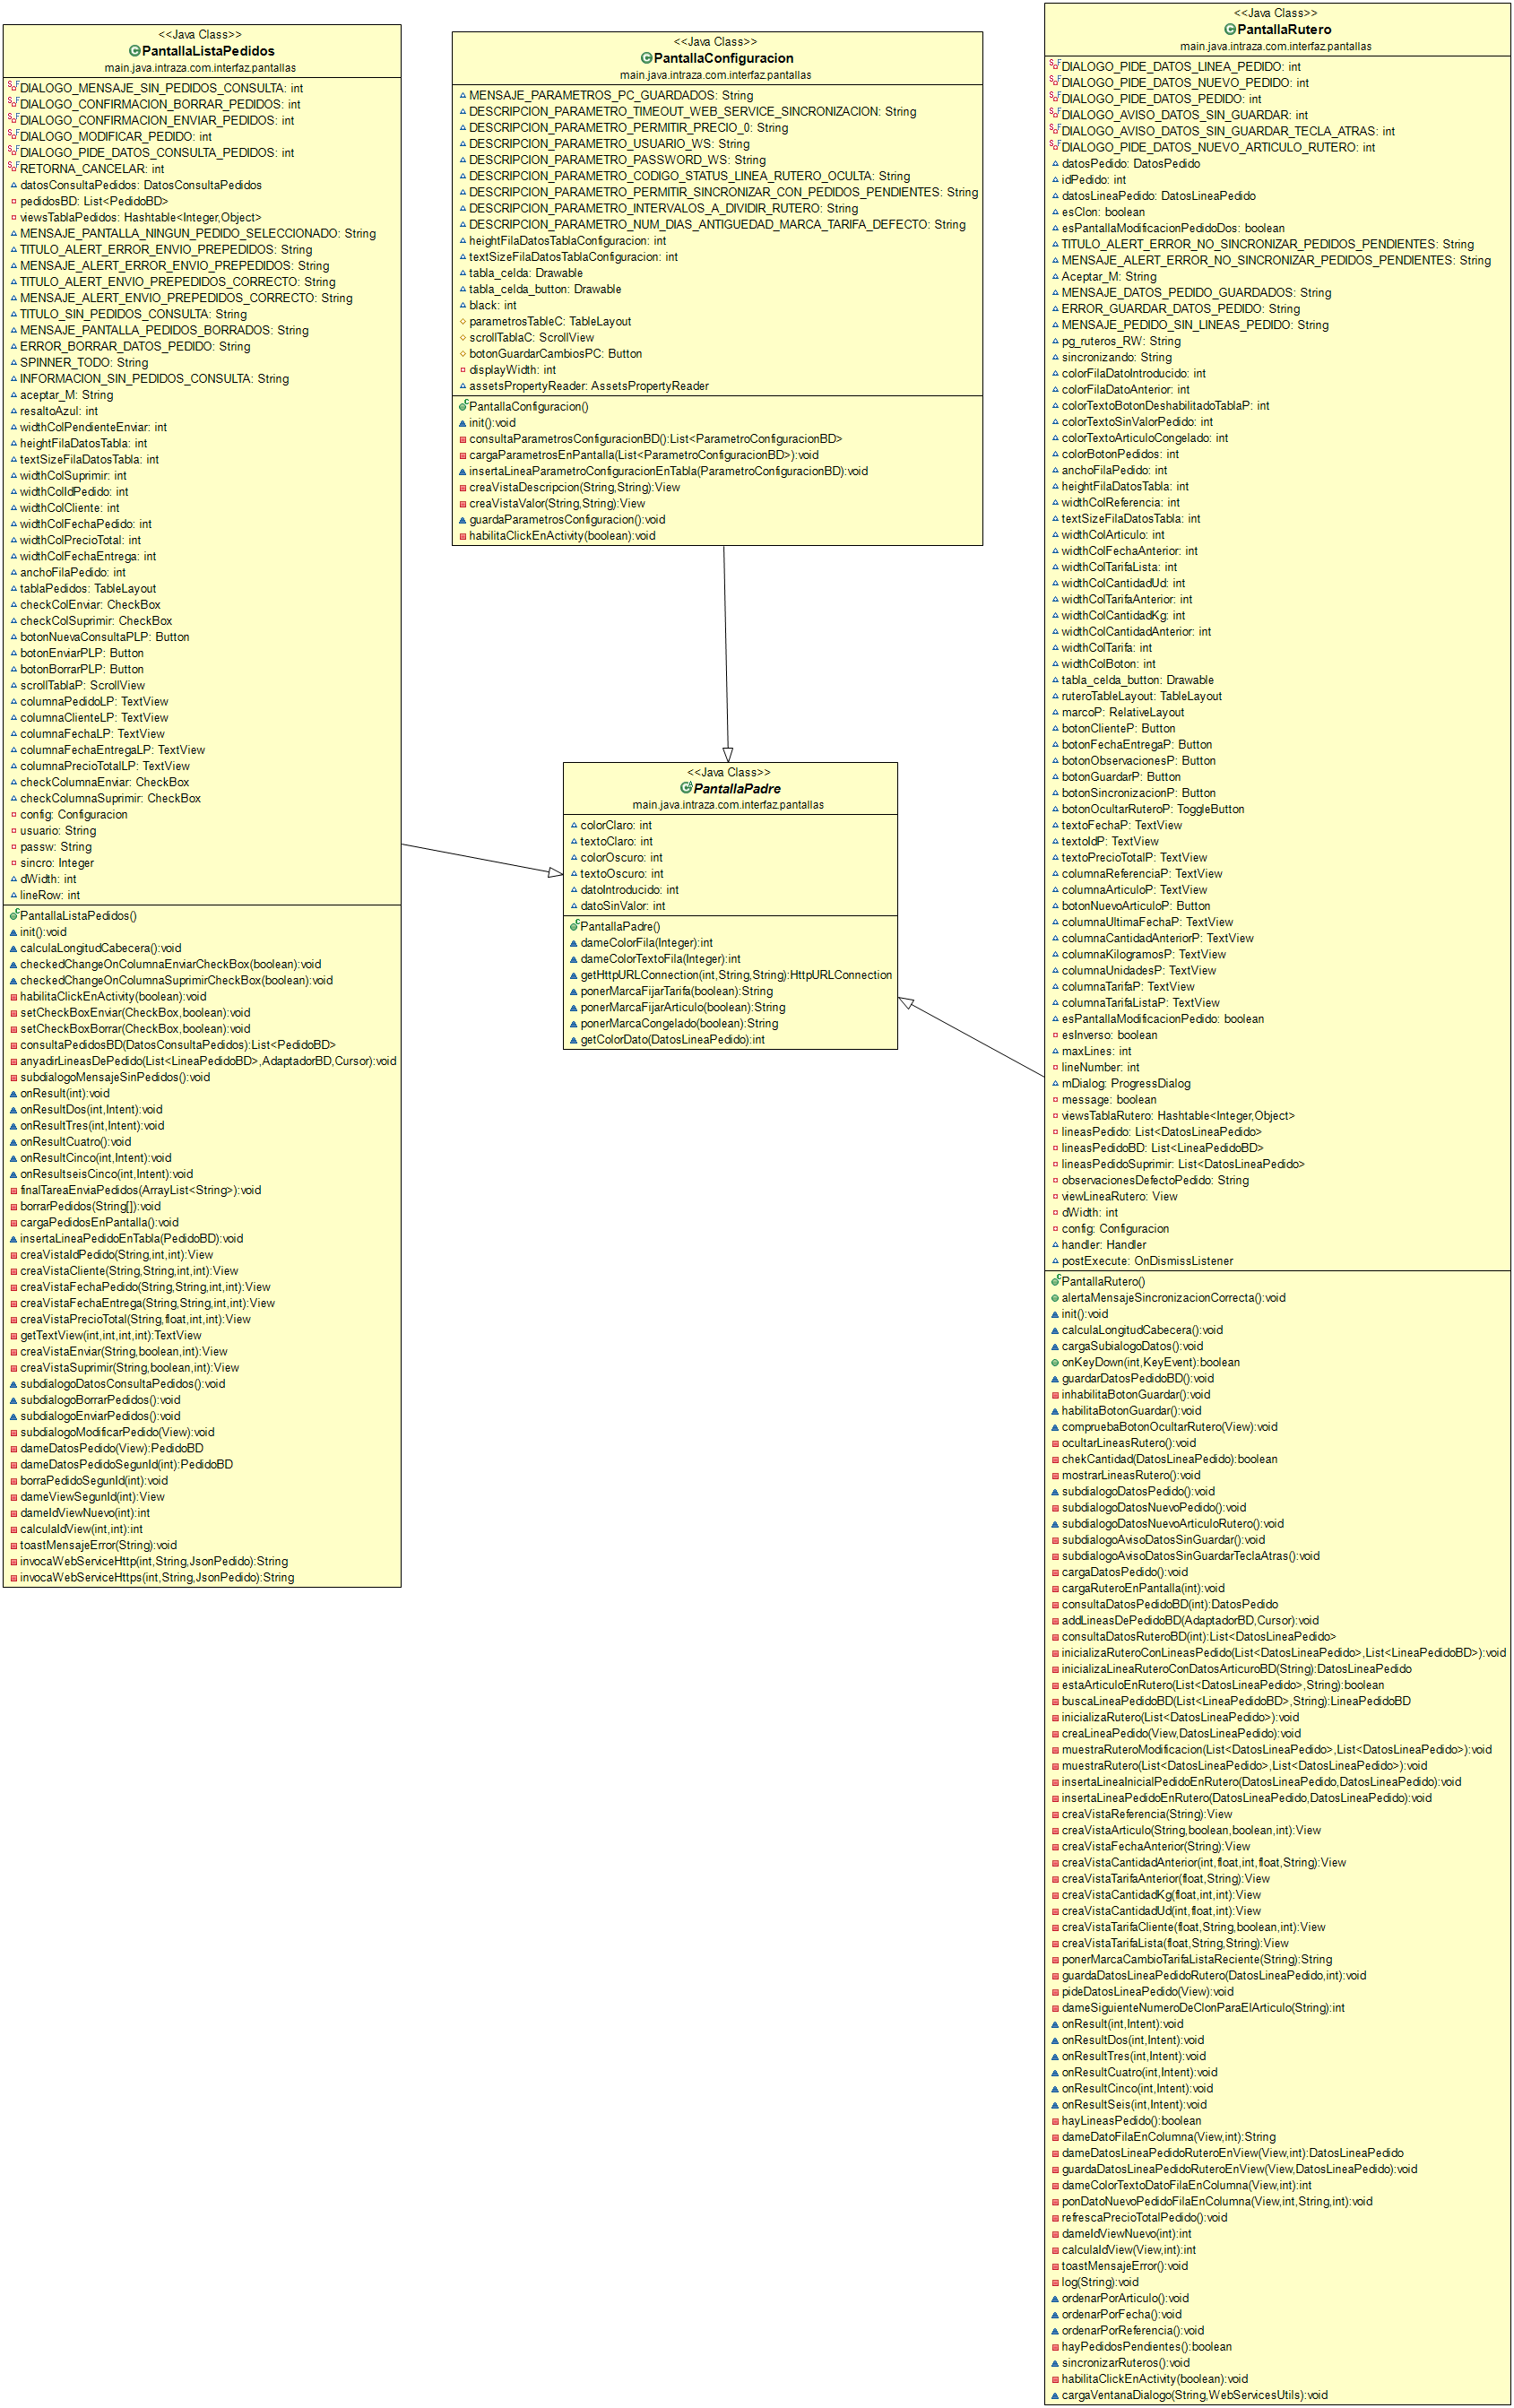
\includegraphics[width=0.8\linewidth]{figuras/and-pantallas}}
	\caption{Relaciones de datos}
	\label{fig:and-pantallas}
\end{figure}

\begin{figure}[H]
	\centering
	\fcolorbox{black}{white}{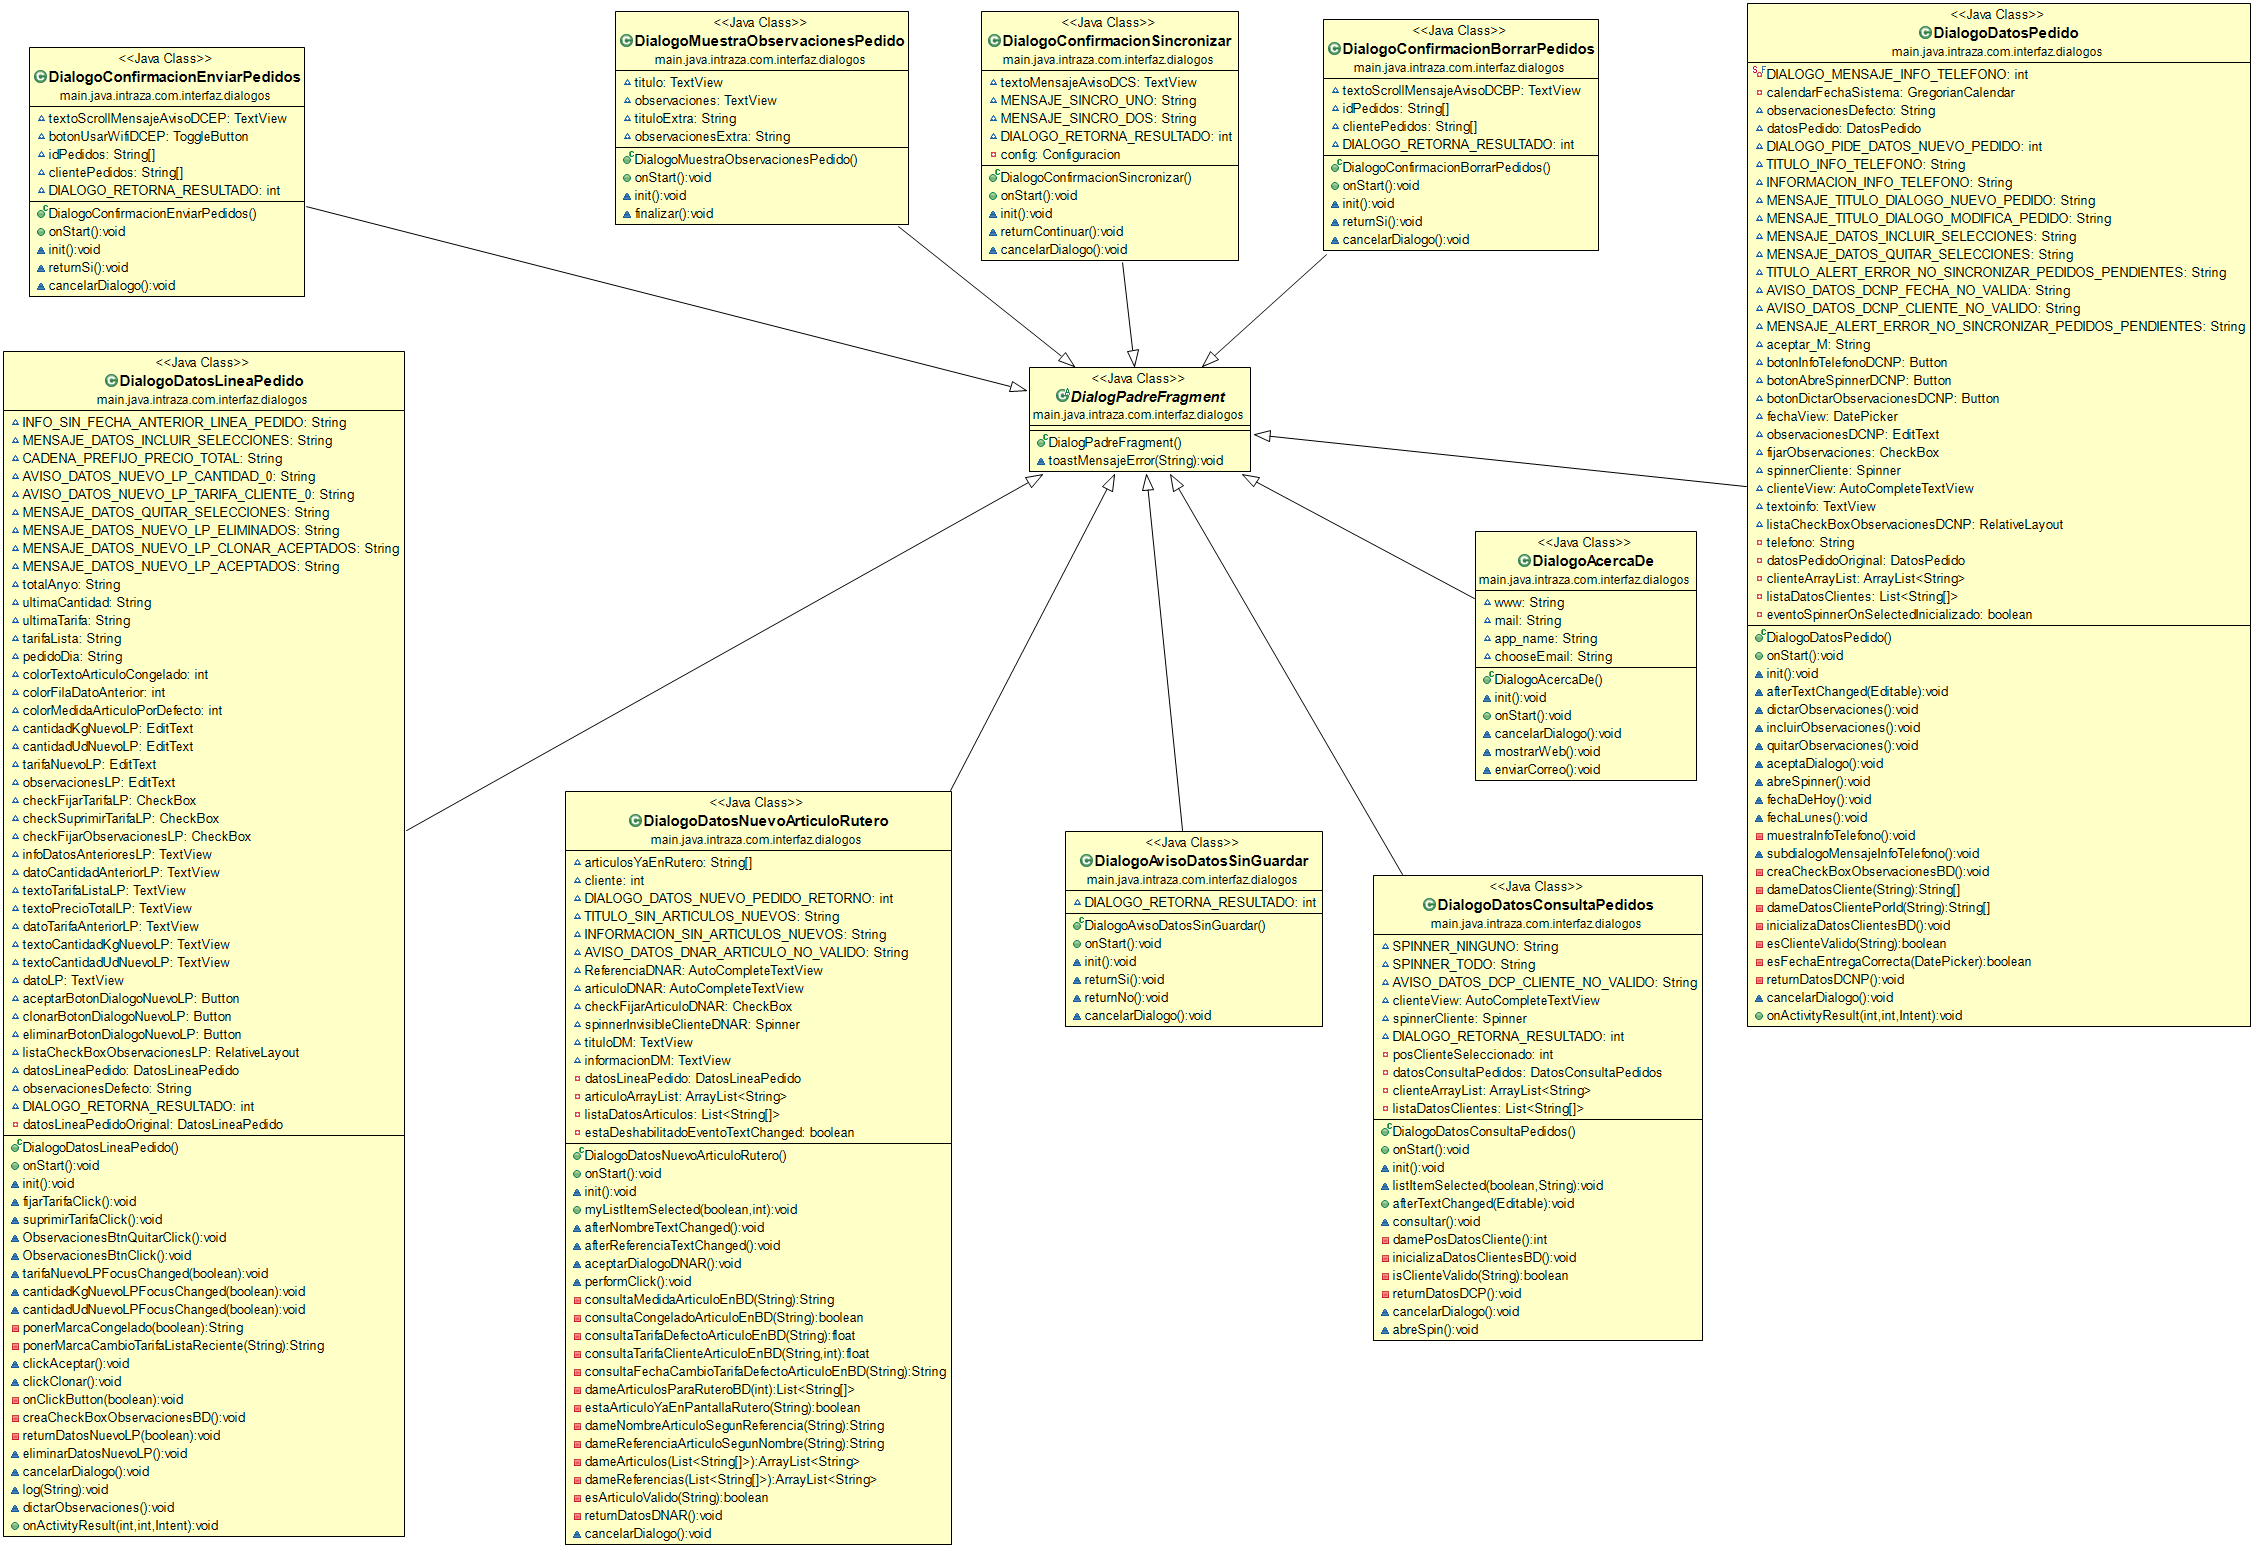
\includegraphics[width=0.7\linewidth]{figuras/and-pantallas-d}}
	\caption{Relaciones de datos}
	\label{fig:and-pantallas-d}
\end{figure}

\begin{figure}[H]
	\centering
	\fcolorbox{black}{white}{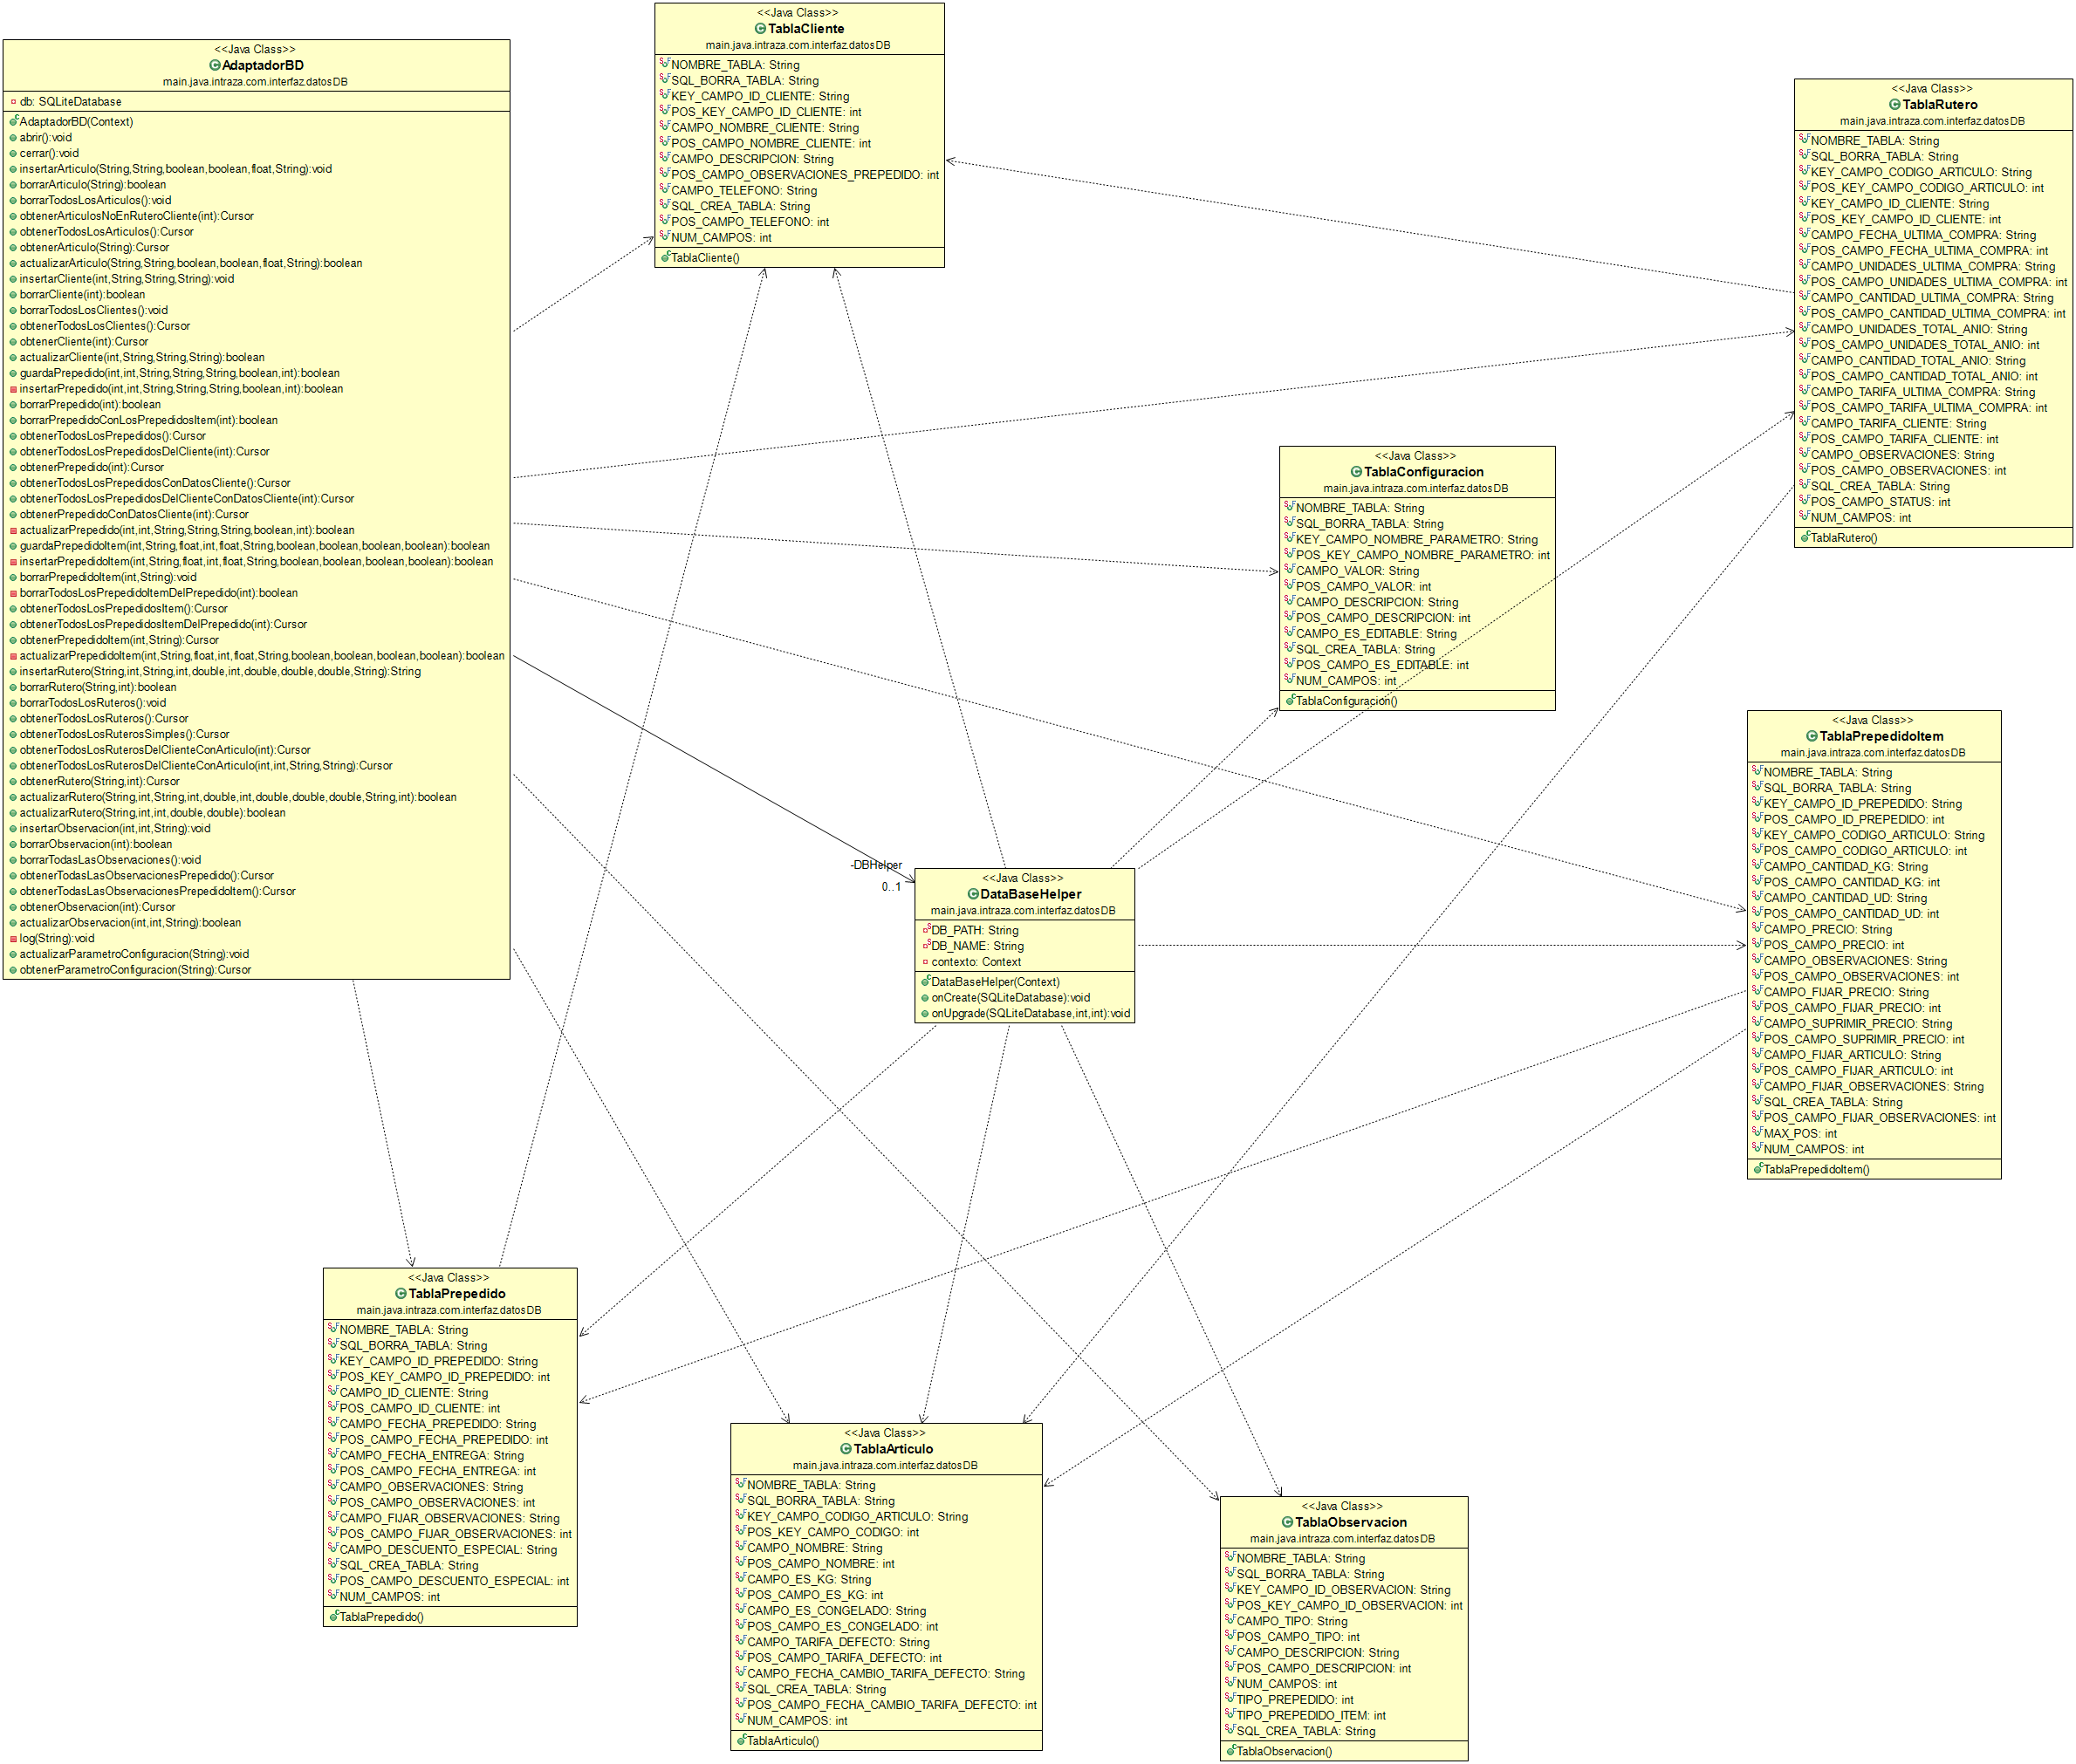
\includegraphics[width=0.7\linewidth]{figuras/and-Db}}
		\caption{Relaciones JSON}
		\label{fig:and-Db}
	\end{figure}

\subsection{Pruebas}

Debido a la imposibilidad de realizar las simulaciones, frente a un entorno de desarrollo de la empresa cliente, por las razones ya expuestas anteriormente, se decide crear una estructura de simulación propia. 

\subsubsection{Desarrollo del ERP de simulación}

Una de las cosas a tener en cuenta, a la hora de desarrollar el ERP\textsuperscript{\textit{[\ref{glo:erp}]}} de pruebas, es que debe ser rápido en su codificación y con una complejidad suficiente para poder realizar todas las pruebas de comunicación.

Con esas premisas, se opta por realizar el aplicativo usando un Framework ligero. La elección es GRAILS\textsuperscript{\textit{[\ref{glo:gra}]}} , un Framework escrito en Groovy y compatible con los entornos JAVA.

El uso de un lenguaje dinámico, de sintaxis parecida a JAVA y su principal peculiaridad de que abarca las tres capas del desarrollo web: acceso a base de datos, capa de negocio y vista, permiten acortar los tiempos de desarrollo notablemente.

Ademas de lo anteriormente dicho, añadiendo herencias y usando reflexión nos encaminan a disponer un producto totalmente operativo en unos pocos días.

\subsubsection{Estructura Básica}

Definiremos una estructura básica compuesta por :
\begin{itemize}	
	\item \textbf{Clases dominio: } Serán el equivalente a las tablas en la base de datos. 
	\item \textbf{Controladores: } Serán los encargados de trazar los flujos de operación, al navegar por las diferentes vistas. 
	\item \textbf{Servicios: } Serán los encargados de proporcionar todas las operaciones de comunicación con agentes externos, filtros y demás código necesario. 
	\item \textbf{Vistas: } Serán las que proporciones las pantallas de la vista del modelo MVC. 
	\item \textbf{TagLibs: } Serán librerías de utilidades para agilizar o simplificar procesos mas complejos en las vistas. 
\end{itemize}

Aquí tenemos un ejemplo de código perteneciente a la clase controlador principal. Corresponde a una acción de listado genérica.
\pagebreak

\begin{lstlisting}[style=JAVA]
private doList() {
	//offset
	doBefore()
	def entidad = clazz
	
	if (entidad) {
		instanceTotal = entidad?.count()
		params.max = Math.min(params.max ? params.int('max') : 10, 100)

	if (params.offset) 
		offset = params.offset
	else if (instanceTotal > offset) 
		params.offset = offset
	
	if (params.sort || !sort)
		instanceList = entidad.list(params)
	else
		instanceList = entidad.list(max: params?.max, offset: params?.offset, sort: sort[0], order: sort[1])
	}
	render(view: 'list', model: mapaVariables(), params: params)
}

\end{lstlisting}

Aquí un ejemplo de acciones de un controlador para el dominio Pedido. Se puede ver que la mayoría del código es procesado por una clase padre, y solo definimos particularidades si lo necesitamos. La creación de nuevas entidades se simplifica, y disponemos de un alto porcentaje de reutilización de código.

\begin{lstlisting}[style=JAVA]
package pedido
import controller.MainController

class PedidoController extends MainController {
	def pedidoService
	def index() 		{ super.doIndex() 			  }
	def list() 			{ super.doList() 			  }
	def create() 		{ super.doCreate() 			  }
	def save() 			{ super.doSave()  			  }
	def show() 			{ super.doShow()  			  }
	def edit() 			{ super.doEdit()  			  }
	def update() 		{ super.doUpdate()  		  }
	def delete() 		{ super.doDelete()    		  }
	def limpiarFiltro() { super.doLimpiarFiltro()     }
	def ajx_filtrar()	{ super.doAjx_filtrar()       }
}
\end{lstlisting}


\subsubsection{Diseño de la base de datos ERP}

Nos planteamos un diseño base de datos sencillo con las tablas básicas que debería tener el ERP. Evidentemente un ERP comercial tendrá mayor complejidad, pero este desarrollo es para realizar un entorno de pruebas. En la figura siguiente planteamos el esquema de tablas y relaciones.

\begin{figure}[H]
	\centering
	\fcolorbox{black}{white}{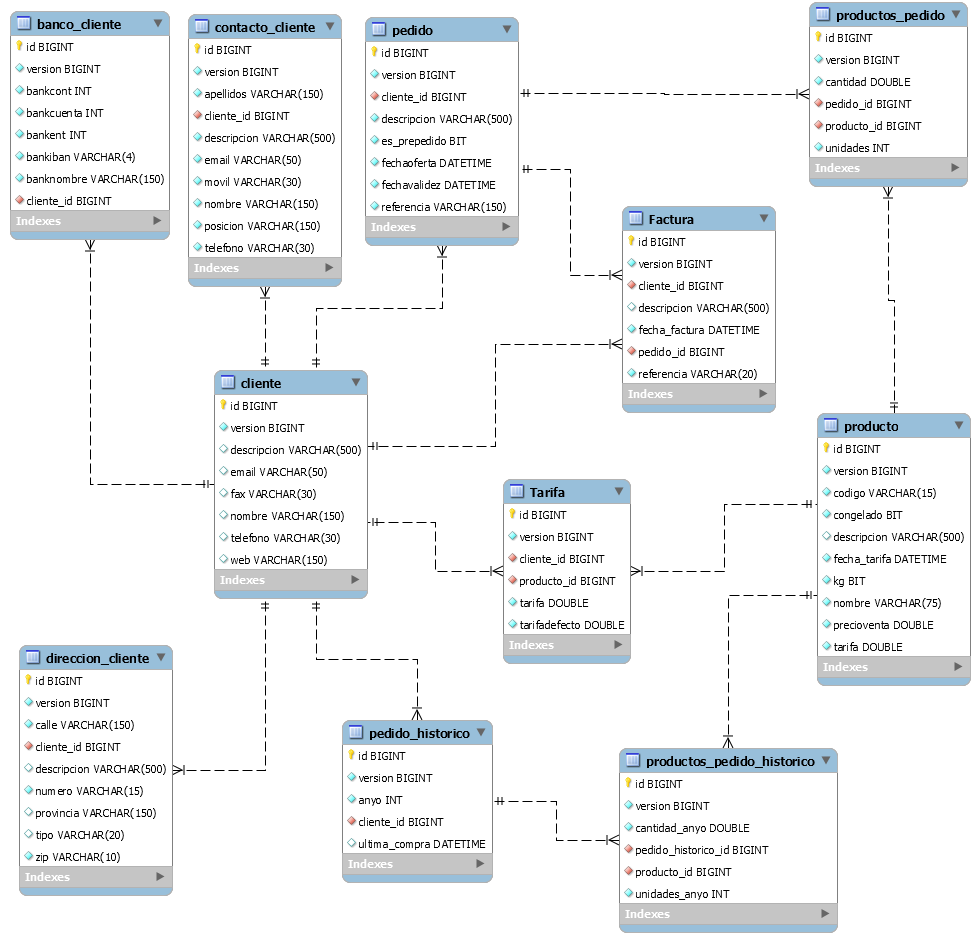
\includegraphics[width=0.7\linewidth]{figuras/grailsM}}
	\caption{Modelo de datos del ERP }
	\label{fig:pruebas-datos}
\end{figure}

\part{Conclusiones}
	\chapter{Conclusiones}


\section{Introducción}

Durante la realización del proyecto se procede a la ejecución de las diferentes fases.  Analizando la viabilidad, planificando a traves de metodologías ágiles SCRUM, se describen  y enumeran las tecnologías y fundamentos teóricos. Se analiza la estructura que evalúa los resultados. En los anexos se definen y aclaran conceptos, además de un manual de usuario y diferentes guías  de instalación y uso de los diferentes componentes. 

\section{Conclusiones}

A continuación vamos a recordar cuál era el Objetivo principal del proyecto marcado al inicio del mismo: 

Construir una aplicación en Android que permita operar con el gestor de pedidos del ERP de la compañía de manera remota. A la finalización del proyecto, se puede afirmar que se ha conseguido satisfacer completamente el Objetivo principal. El grado de consecución se puede considerar bastante alto, resaltando el hecho de que la empresa empezó a operar con la app en la campaña de verano, sin incidentes reseñables. 

El sistema/módulo desarrollado cumple perfectamente el objetivo propuesto y además está totalmente preparado para realizar futuras ampliaciones e integraciones. 

La consecución del Objetivo principal incluía la satisfacción de unos sub-objetivos que van totalmente ligados. A continuación se describen los que se han satisfecho: 

- El principal objetivo a cumplir a nivel personal fue adquirir conocimientos sobre el entorno y el contexto del proyecto.

Siendo estos variados como:
\begin{itemize}
	\item \emph{\textbf{Conocer las principales características del lenguaje Java:}} Sin tener un previo conocimiento básico del lenguaje Java habría sido imposible programar la aplicación en Android. 

	\item \emph{\textbf{Conocer las principales características de Android:}} Al igual que en el punto anterior, si no se hubiera estudiado y entendido las principales características de Android, así como su funcionamiento, llevar a cabo este proyecto con el desarrollo de la aplicación habría sido imposible. 

	\item \emph{\textbf{Estudiar el entorno de desarrollo de Android:}} Con la elección del entorno Android studio, fue necesario estudiarlo, entenderlo y manipularlo con la suficiente soltura que nos permitiera el correcto desarrollo de la aplicación. 

	\item \emph{\textbf{Conocer funcionamiento y desarrollo de aplicaciones J2EE:}}
Sin este conocimiento, habría sido imposible desarrollar el servicio web de conexión.

	\item \emph{\textbf{Conocer funcionamiento y manejo de bases de datos:}} Sin este conocimiento, no podríamos abordar la persistencia de datos solicitada. 

	\item \emph{\textbf{Conocer funcionamiento y manejo de servidores de aplicaciones java:}} Era necesario conocer los diferentes entornos de hospedaje de aplicaciones, ya sea tomcat, jboss, websphere, etc. 
	
\end{itemize}

Otro de los objetivos a cumplir en este proyecto era la realización de la memoria de proyecto debidamente cumplimentada con el reglamento existente. 

\section{Planificación temporal final}

Por otro lado estaba el factor temporal. El proyecto se debía ajustar a una planificación realizada al comienzo del mismo. La duración era de 3 meses aproximadamente. Ya que se quería tener operativa la aplicación antes de la campaña de verano, de vital importancia para la empresa. 

Pero por lo general, a la finalización del proyecto, se puede afirmar que se ha logrado seguir bastante bien la planificación temporal realizada en su comienzo, siempre con las pequeñas y lógicas desviaciones. 

\section{Conclusión final}

Con lo visto anteriormente, podemos afirmar que, a la finalización del proyecto, el grado de consecución de objetivos es bastante alto y que se ha logrado ajustar bastante bien su desarrollo en el espacio temporal planificado. Por tanto, se puede concluir que el proyecto ha finalizado con éxito. 




\part {Anexos}
	\chapter{ANEXO I}
\section{Conceptos y aclaraciones}

\subsection{Maven}
\label{glo:maven}
\textbf{Maven} es una herramienta de software para la gestión y construcción de proyectos Java creada por Jason van Zyl, de Sonatype, en 2002. Es similar en funcionalidad a \textbf{Apache Ant }, pero tiene un modelo de configuración de construcción más simple, basado en un formato XML. Estuvo integrado inicialmente dentro del proyecto Jakarta pero ahora ya es un proyecto de nivel superior de la Apache Software Foundation.

Maven utiliza un \textbf{POM\textit{(Project Object Model)} }para describir el proyecto de software a construir, sus dependencias de otros módulos y componentes externos, y el orden de construcción de los elementos. Viene con objetivos predefinidos para realizar ciertas tareas claramente definidas, como la compilación del código y su empaquetado. Una característica clave de Maven es que está listo para usar en red. El motor incluido en su núcleo puede dinámicamente descargar plugins de un repositorio, el mismo repositorio que provee acceso a muchas versiones de diferentes proyectos Open Source en Java, de Apache y otras organizaciones y desarrolladores. Este repositorio y su sucesor reorganizado, el repositorio Maven 2, pugnan por ser el mecanismo de facto de distribución de aplicaciones en Java, pero su adopción ha sido muy lenta. Maven provee soporte no solo para obtener archivos de su repositorio, sino también para subir artefactos al repositorio al final de la construcción de la aplicación, dejándola al acceso de todos los usuarios. Una caché local de artefactos actúa como la primera fuente para sincronizar la salida de los proyectos a un sistema local. \cite{maven}

\subsection{Gradle}
\label{glo:gradle}
\textbf{Gradle} es un sistema de automatización de construcción de código abierto que construye sobre los conceptos de Apache Ant y Apache Maven e introduce un lenguaje especifico del dominio (DSL) basado en Groovy en vez de la forma XML utilizada por Apache Maven para declarar la configuración de proyecto. \textbf{Gradle} utiliza un \textbf{DAG \textit{(Grafo Acíclico Dirigido)}} para determinar el orden en el que las tareas pueden ser ejecutadas.
\textbf{Gradle} fue diseñado para construcciones multi-proyecto las cuáles pueden crecer para ser bastante grandes, y da apoyo a construcciones incrementales determinando inteligentemente qué partes del árbol de construcción están actualizadas, de modo que cualquier tarea dependiente a aquellas partes no necesitarán ser re-ejecutada.\cite{gradle}

\subsection{Anotación Java}
\label{glo:anota}

En programación, una Anotación Java es una forma de añadir meta-datos al código fuente Java que están disponibles para la aplicación en tiempo de ejecución. Muchas veces se usa como una alternativa a la tecnología XML.

Las Anotaciones Java pueden añadirse a los elementos de programa tales como clases, métodos, campos, parámetros, variables locales, y paquetes. Al contrario que las etiquetas añadidas a la documentación Java y procesadas con las herramientas tales como XDoclet, las Anotaciones Java son completamente accesibles al programador, mientras que el software se ejecuta, usando reflexión.

\subsection{ERP}
\label{glo:erp}

El término ERP se refiere a Enterprise Resource Planning, que significa sistema de planificación de recursos empresariales. Estos programas se hacen cargo de distintas operaciones internas de una empresa, desde producción a distribución o incluso recursos humanos.

Además, los ERP ofrecen integración con soluciones de BI o Business Intelligence, permitiendo realizar informes sobre el estado de su empresa directamente con los datos del sistema ERP. Esto ofrece un nivel de conocimiento detallado y actualizado del estado de la empresa que resulta indispensable a la hora de analizar y mejorar procesos internos como el marketing y ventas, la organización u otros aspectos clave de una compañía.

\subsection{Framework}
\label{glo:frwk}
Un Framework es básicamente un entorno de desarrollo, en el que los podemos desarrollar mucho mas fácil y rápidamente aplicaciones de todo tipo, incluso las aplicaciones web. Un Framework puede estar constituido de librerías de código fuente, utilidades, plugins, modelos de desarrollo, y todo tipo de herramientas cuyo único propósito de acelerar el ritmo de desarrollo de una aplicación. 

\subsection{Grails}
\label{glo:gra}

Grails (Groovy and rails). Es básicamente un Framework de desarrollo de aplicaciones web, en el que usamos principalmente el lenguaje de Java y Groovy, incluso se puede combinar el código.Es un Framework que funciona bajo un modelo conocido como MVC (modelo vista controlador), en el que principalmente lo que se hace es crear “Controladores” que son como servicios que manipulan nuestra aplicación web, y todo el código de estos controladores es ejecutado en el servidor web.

Ademas Grails utiliza plantillas y vistas. No solo podemos programar controladores, si no que podemos utilizar un lenguaje llamado groovy server pages(GSP) para poder programar directamente sobre lo que seria nuestra pagina web con código HTML, es como si programáramos en jsp o php, esto nos da mucha flexibilidad y orden al programar nuestras aplicaciones web. 

Dispone de gran cantidad de plugins para realizar múltiples desarrollos, conversores, etc...

\chapter{ANEXO II}
\section{Manual de usuario}

\subsection{Pantalla principal}

Esta pantalla se compone de 5 botones de acción.

\begin{itemize}
	\item \textbf{Crear pedidos:} Lanza el proceso para la creación de pedidos.
	\item \textbf{Gestión de pedidos:} Lanza el proceso para la gestión de pedidos.
	\item \textbf{Sincronizar con InTraza:} Lanza el proceso de sincronización con el ERP.
	\item \textbf{Acerca de:} Ventana informativa.
	\item \textbf{Configuración:} Por medio de una contraseña permite cambiar algunos parámetros de la aplicación.
					
\end{itemize}

\begin{figure}[H]
	\centering
	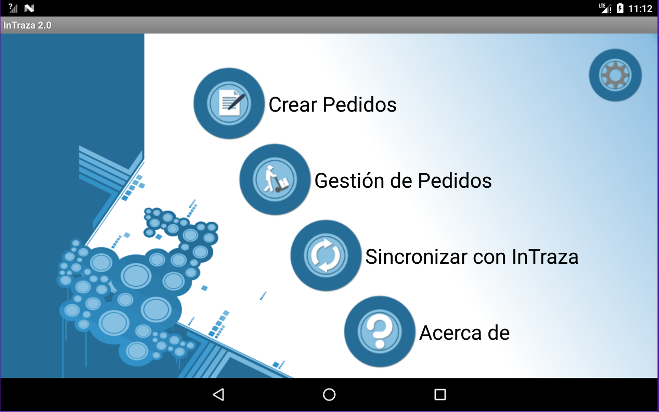
\includegraphics[width=0.65\linewidth]{figuras/manual/p1}
	\caption{Intraza - pantalla principal}
	\label{fig:Itzp1}
\end{figure}

\subsection{Creación de pedidos}

En esta pantalla elegiremos el cliente por medio del combo, además de la fecha de entrega y observaciones del pedido. Las observaciones pueden dictarse, escribirse o elegirse de una lista predefinida para ese cliente. Cuando seleccionas fijar observaciones añades estas a la lista de observaciones prefijadas. 

\begin{figure}[H]
	\centering
	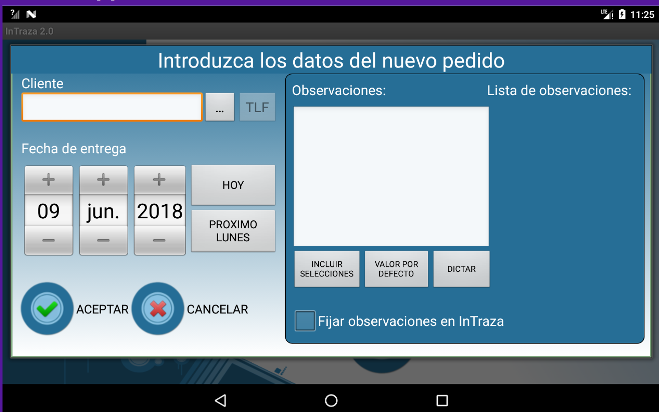
\includegraphics[width=0.65\linewidth]{figuras/manual/p3}
	\caption{Intraza - creación de pedidos}
	\label{fig:Itzp2}
\end{figure}

Una vez validada la pantalla anterior, nos muestra una pantalla a la que llamaremos ruteros que muestra las lineas de pedido de la empresa seleccionada y nos permite crear adicionales. Podremos mostrar/ocultar las lineas antiguas y volver a la pantalla anterior si queremos cambiar algo, por medio de los botones. Ademas podremos sincronizar los ruteros de la empresa seleccionada.

\begin{figure}[H]
	\centering
	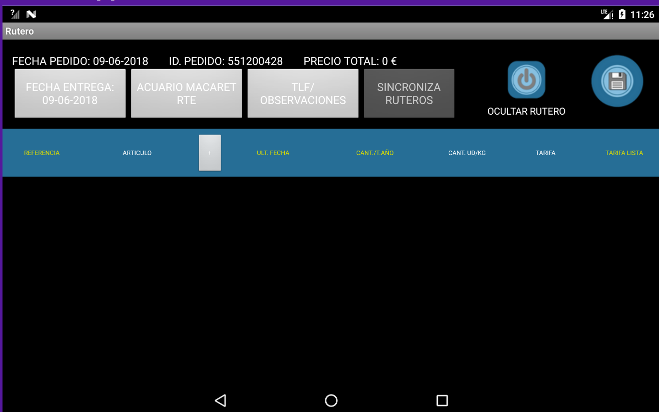
\includegraphics[width=0.65\linewidth]{figuras/manual/p2}
	\caption{Intraza - ruteros}
	\label{fig:Itzp3}
\end{figure}

\pagebreak

Una vez pulsado el botón de añadir artículo '(+)' nos mostrará un ventana de dialogo para elegir el artículo que queremos introducir. 

\begin{figure}[H]
	\centering
	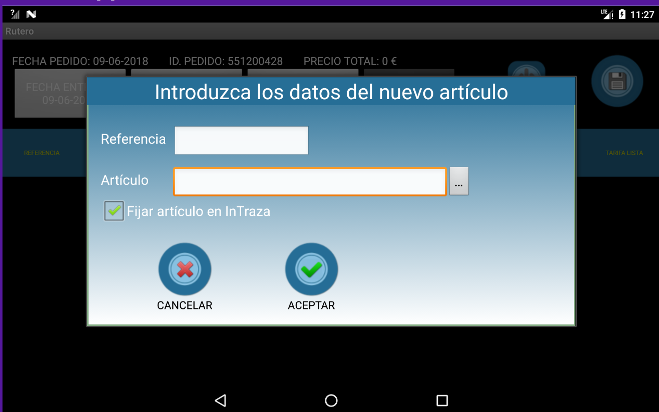
\includegraphics[width=0.7\linewidth]{figuras/manual/p4}
	\caption{Intraza - introducir articulo}
	\label{fig:Itzp4}
\end{figure}

Una vez aceptado el articulo nos mostrará la pantalla para rellenar los campos necesarios para el pedido. Ademas nos permitirá clonar un rutero para pedidos repetitivos.

\begin{figure}[H]
	\centering
	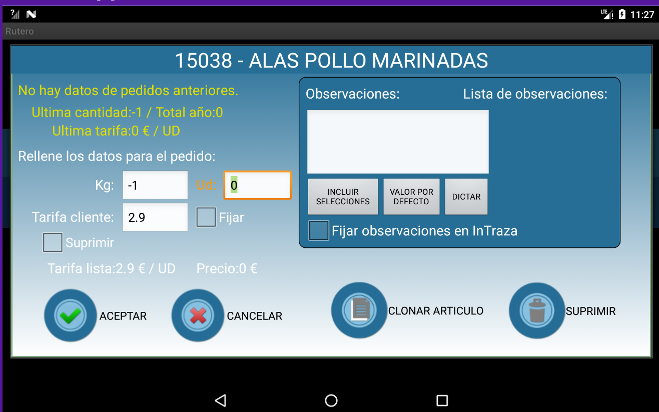
\includegraphics[width=0.7\linewidth]{figuras/manual/p5}
	\caption{Intraza - rellenar cantidades/observaciones}
	\label{fig:Itzp5}
\end{figure}

\pagebreak
Una ver añadido el articulo podemos comprobar que la pantalla ruteros dispone de una linea con los datos del mismo.

\begin{figure}[H]
	\centering
	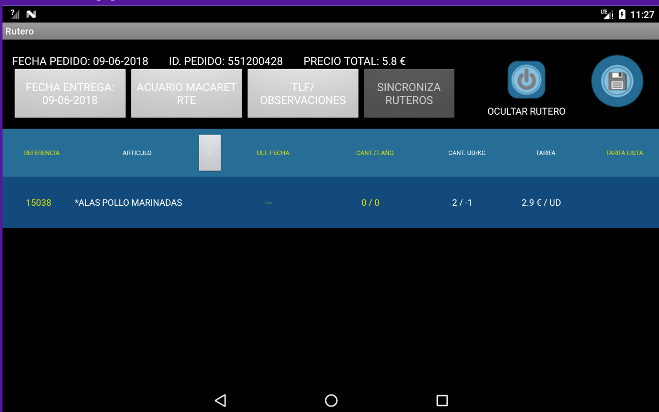
\includegraphics[width=0.7\linewidth]{figuras/manual/p6}
	\caption{Intraza - articulo insertado}
	\label{fig:Itzp6}
\end{figure}

\subsection{Gestión de pedidos}

En esta pantalla podremos elegir todos los pedidos o elegir los pedidos del cliente que queremos visualizar.

\begin{figure}[H]
	\centering
	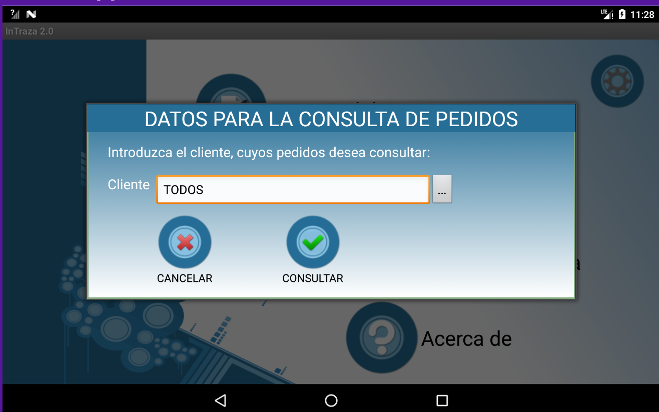
\includegraphics[width=0.7\linewidth]{figuras/manual/p7}
	\caption{Intraza - gestión de pedidos}
	\label{fig:Itzp7}
\end{figure}

\pagebreak
En esta pantalla podremos gestionar los pre-pedidos que están almacenados en el dispositivo. Podremos ver su contenido clickando en el id de pedido. Ademas podremos borrarlos o enviarlos a la central, para que pasen a ser parte del ERP.

\begin{figure}[H]
	\centering
	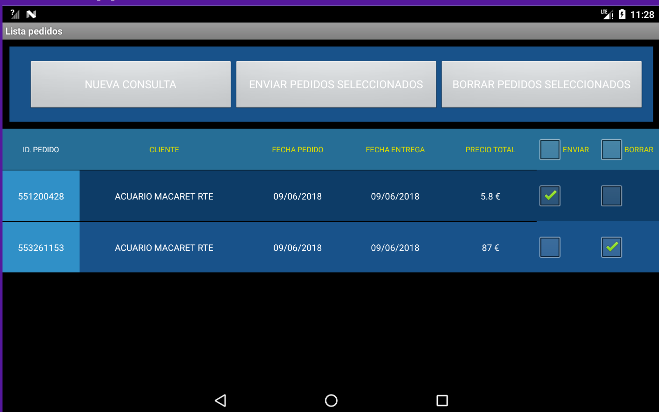
\includegraphics[width=0.7\linewidth]{figuras/manual/p9}
	\caption{Intraza - lista de pedidos}
	\label{fig:Itzp8}
\end{figure}

\subsection{Sincronizar con Intraza}

Por medio de esta pantalla podremos sincronizar los datos guardados en el ERP, con los datos de la aplicación. Sincronizará clientes, artículos y ruteros.

\begin{figure}[H]
	\centering
	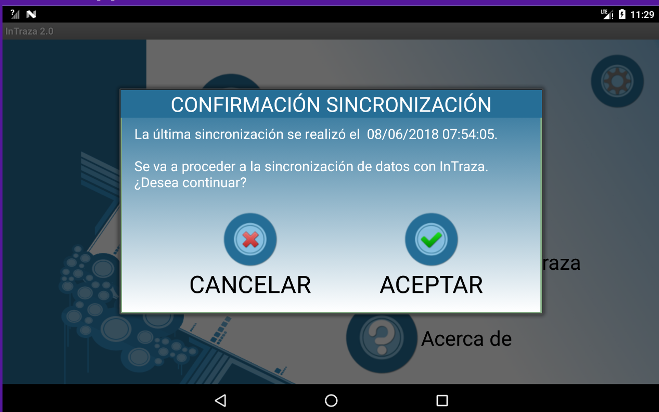
\includegraphics[width=0.7\linewidth]{figuras/manual/p10}
	\caption{Intraza - sincronización}
	\label{fig:Itzp9}
\end{figure}

\subsection{Configuración}

En esta pantalla podremos configurar el valor de algunos parámetros de la aplicación. Como por ejemplo la ruta del WebService de comunicaciones. Esta pantalla está protegida con contraseña.

\begin{figure}[H]
	\centering
	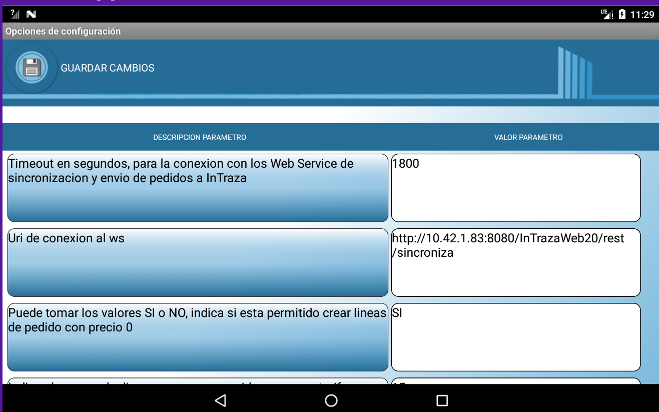
\includegraphics[width=0.7\linewidth]{figuras/manual/p8}
	\caption{Intraza - configuración}
	\label{fig:Itzp10}
\end{figure}


	\chapter{ANEXO III}

\section{Guías de Instalación}

\subsection{Instalación del Sistema Máquina Virtual Ubuntu}

\subsubsection{Máquina virtual Ubuntu}

Una vez instalado la aplicación virtual box, crearemos una maquina nueva. Pulsamos a nueva, Ubuntu. Como tipo seleccionamos: Linux y la versión la que deseemos: Ubuntu 64 bits. 

\begin{figure}[H]
	\centering
	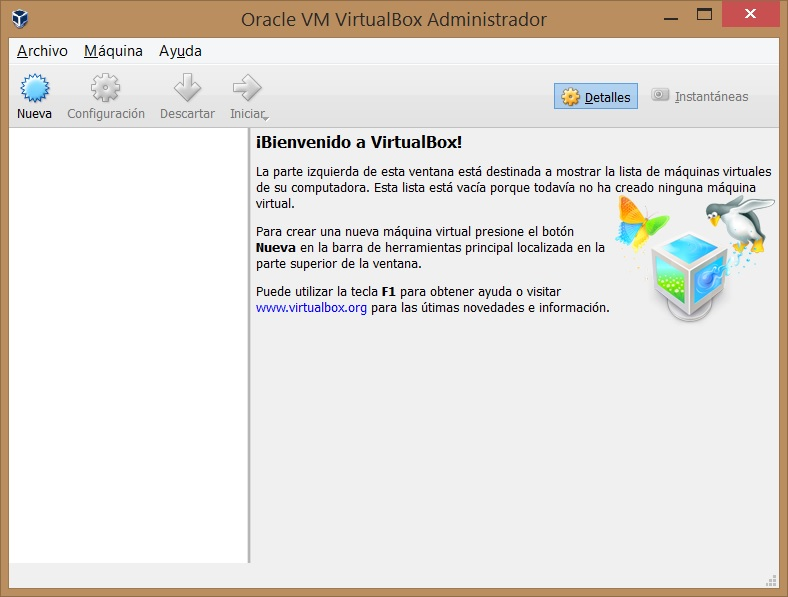
\includegraphics[width=0.7\linewidth]{figuras/vm-1}
	\caption{Virtual box - inicio}
	\label{fig:vm1}
\end{figure}

Le asignamos la memoria RAM a la máquina virtual 2048 MB es el mínimo recomendado, yo he usado 4.096 MB. Seleccionamos la opción \textit{Crear un disco duro virtual ahora}, ya que no tenemos ninguno creado anteriormente y hacemos clic en \underline{Crear} y seleccionamos en la siguiente pantalla la opción VDI (Virtual BOX Disk Image) y con tamaño “Reservado Dinámico” para que ocupe lo que realmente necesite.

\begin{figure}[H]
	\centering
	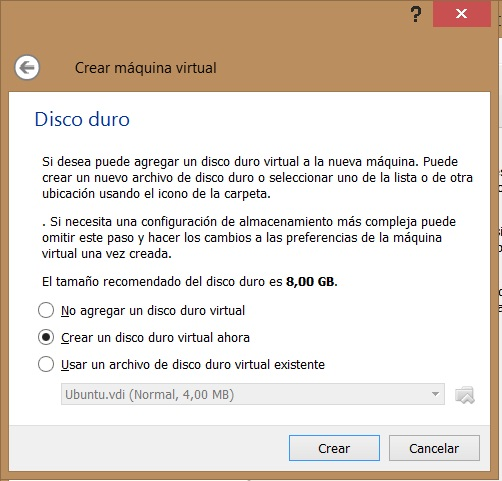
\includegraphics[width=0.5\linewidth]{figuras/vm-2}
	\caption{Virtual box - crear disco duro}
	\label{fig:vm2}
\end{figure}

Ya tenemos creada la máquina virtual. Solo nos queda empezar a instalar Ubuntu en el siguiente apartado.

\begin{figure}[H]
	\centering
	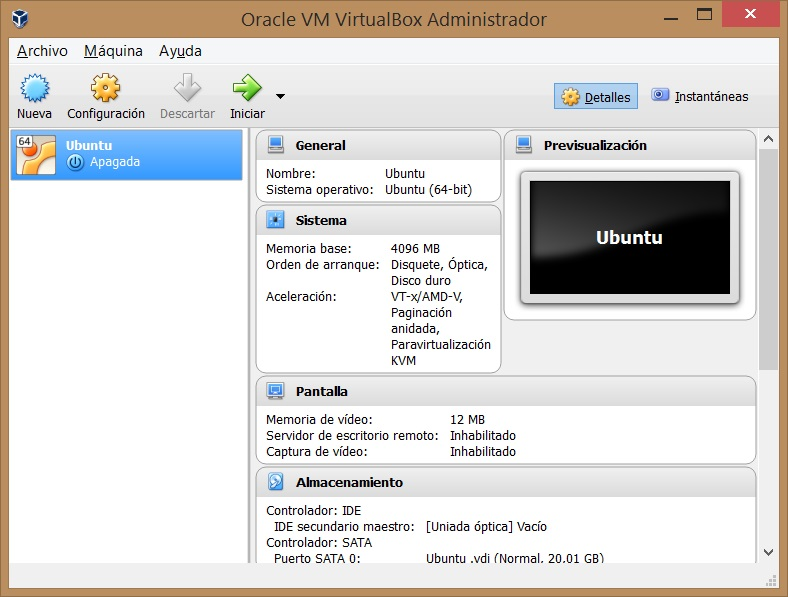
\includegraphics[width=0.6\linewidth]{figuras/vm-3}
	\caption{Virtual box-vm creada}
	\label{fig:vm3}
\end{figure}

Pulsamos sobre \textit{iniciar} para arrancar la máquina virtual y empezar la instalación de Ubuntu, nos pedirá que seleccionemos la imagen ISO que hemos descargado anteriormente. La instalación comienza con un asistente de instalación en el que debemos seleccionar el idioma a usar y pulsar en “instalar Ubuntu”. Su instalación ha sido bastante rápida, nos ha llevado un total de 9 minutos.

\begin{figure}[H]
	\centering
	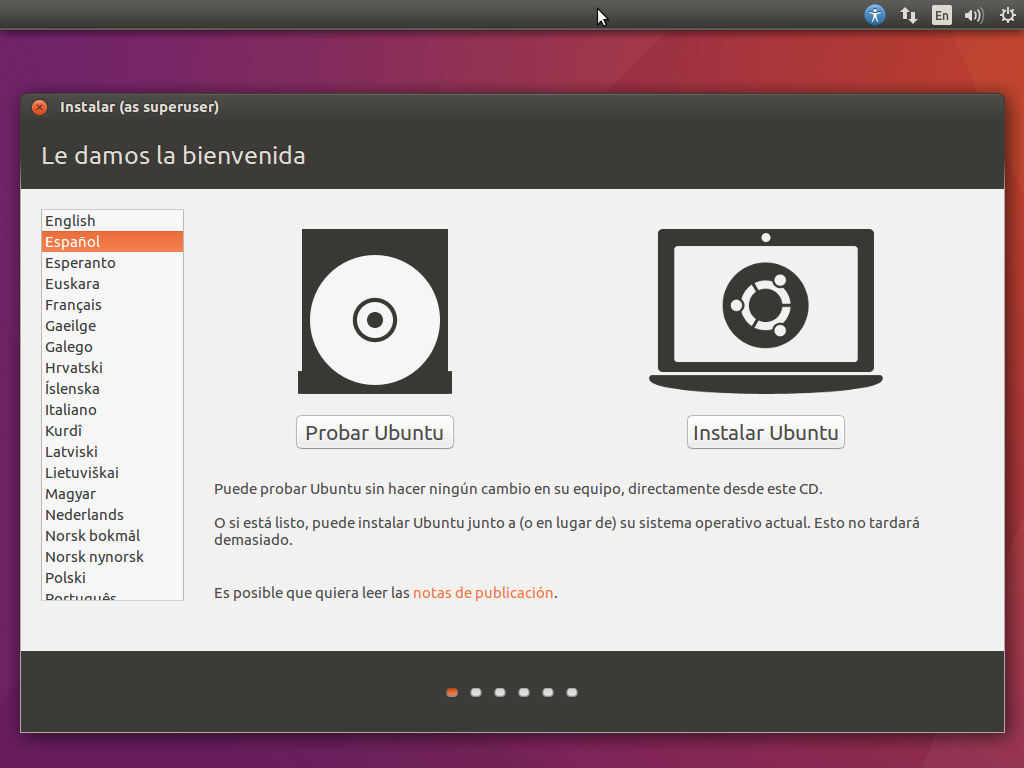
\includegraphics[width=0.7\linewidth]{figuras/vm-4}
	\caption{Instalación ubuntu}
	\label{fig:vm4}
\end{figure}

En la siguiente pantalla nos da la opción de descargar las actualizaciones e instalar software de terceros para reproducir archivos multimedia y otros. A continuación, nos saldrá el asistente del particionado del disco duro, en este caso vamos a usar todo el disco virtual que hemos creado por lo que dejamos la opción por defecto y pulsamos en \textit{instalar ahora}
Configuramos las particiones por defecto, seleccionamos nuestra zona horaria y pulsamos en \textit{continuar}, y elegimos nuestra distribución del teclado y \textit{continuar}. Luego nos saldrá una última pantalla en la que deberemos poner nuestro nombre de usuario y contraseña. También podemos seleccionar la opción de inicio de sesión automático.

\begin{figure}[H]
	\centering
	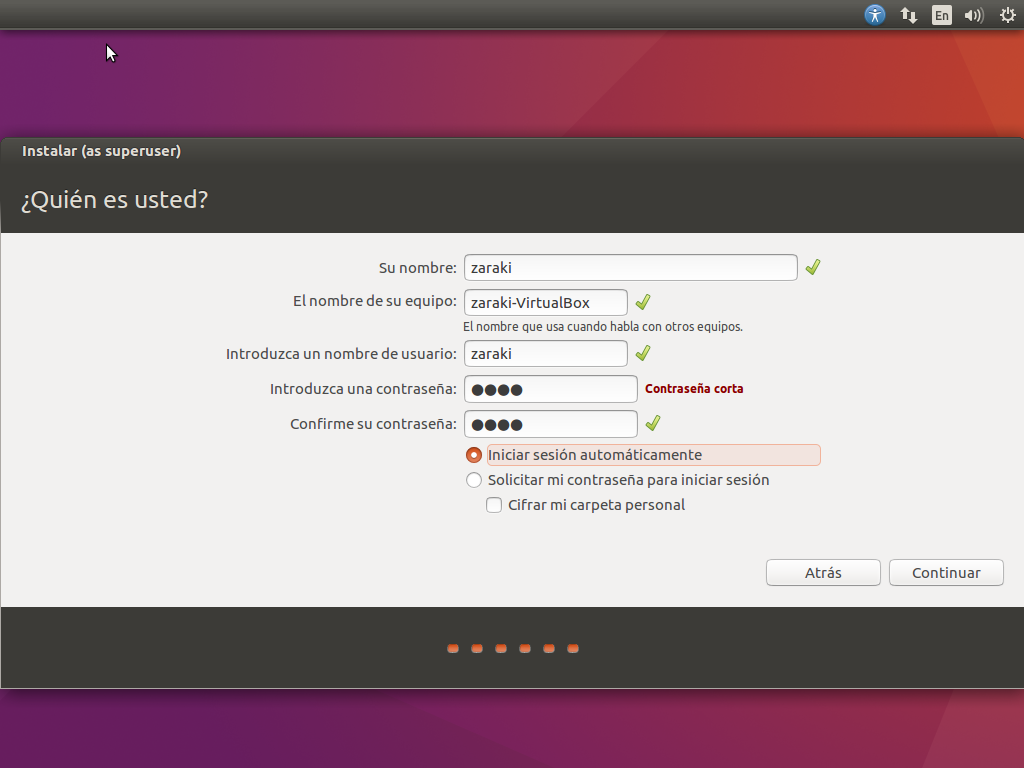
\includegraphics[width=0.8\linewidth]{figuras/vm-5}
	\caption{Instalación ubuntu - usuario y password}
	\label{fig:vm5}
\end{figure}

Finalmente reiniciamos nuestro sistema y ya tendremos un Ubuntu 16.04 LTS funcionando.

\subsection{Instalar Eclipse}
Instalar el JDK de Oracle
En un principio debemos verificar si disponemos de una versión de desarrollo de java instalada. Se detallan los comandos para verificar instalar en modo consola.

\begin{lstlisting}

java -version
sudo apt-get update
sudo apt-get install python-software-properties
sudo add-apt-repository ppa:webupd8team/java
sudo apt-get install oracle-java8-installer
\end{lstlisting}

Una Vez instalada se puede comprobar la instalación.

\begin{figure}[H]
	\centering
	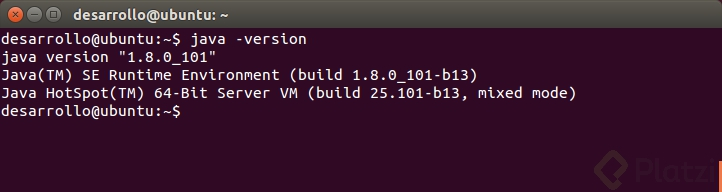
\includegraphics[width=0.7\linewidth]{figuras/ecli-1}
	\caption{Terminal ubuntu}
	\label{fig:ecli1}
\end{figure}

Descargar e Instalar Eclipse Oxigen
Ir a la página oficial y descargar la última versión para Linux 64 bits. Se extrae el archivo de la carpeta y se mueve la carpeta a otra ubicación más cómoda.

\begin{lstlisting}

sudo mkdir -p /opt/ide/64
sudo mv ~/Downloads/eclipse /opt/ide/64
cd /opt/ide/64
sudo chown -R root:root eclipse
sudo ln -sf /opt/ide/64/eclipse/eclipse /usr/bin/

\end{lstlisting}

\begin{figure}[H]
	\centering
	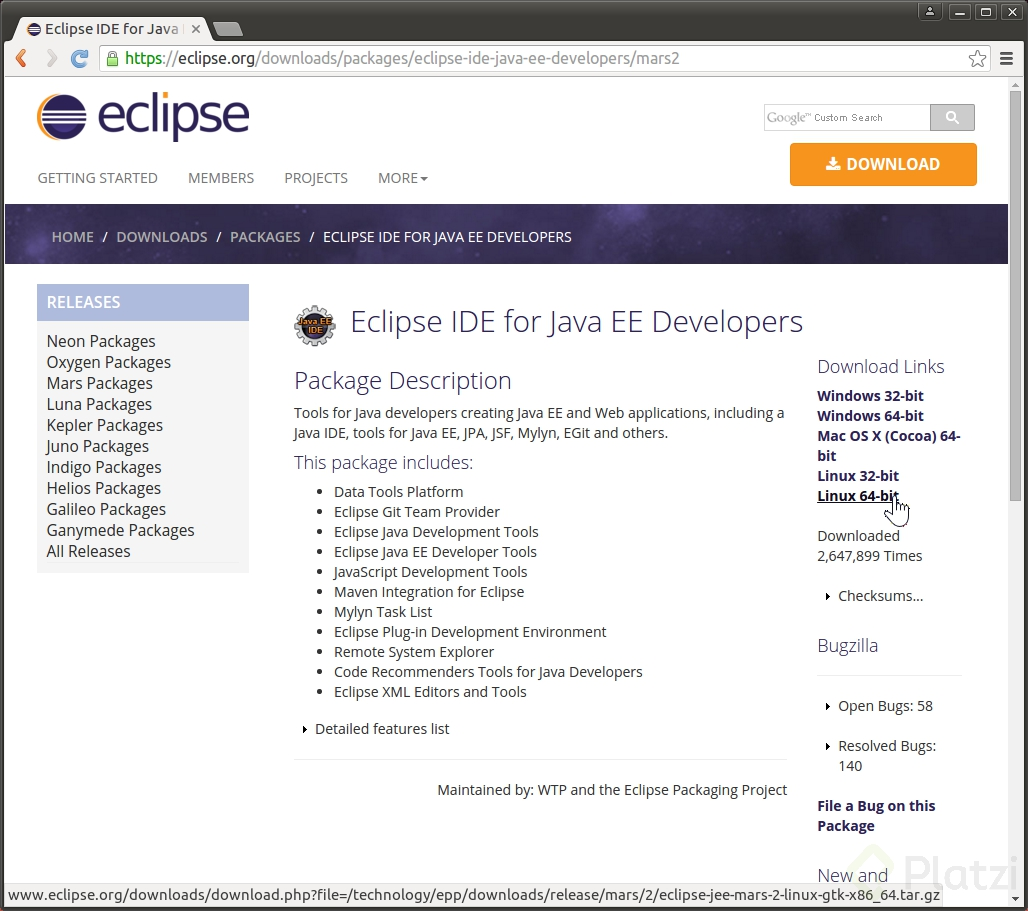
\includegraphics[width=0.6\linewidth]{figuras/ecli-2}
	\caption{Ventana Eclipse}
	\label{fig:ecli2}
\end{figure}


Definir Eclipse como un programa para su acceso directo
Se ejecuta el siguiente comando, lo cual abrirá una carpeta dónde se encuentran las aplicaciones del sistema con todos los permisos para administrarlos.

\begin{lstlisting}

sudo nautilus /usr/share/applications
\end{lstlisting}

Para generar un acceso directo a eclipse. Eclipse.desktop

\begin{lstlisting}

sudo mv /usr/share/applications/Eclipse.desktop /usr/share/applications/eclipse-mars-2.desktop
sudo gedit /usr/share/applications/eclipse-mars-2.desktop
[Desktop Entry]
Name=Eclipse Mars 2
Comment=IDE for Java
Exec=/usr/bin/eclipse
Icon=/opt/ide/64/eclipse/icon.xpm
Terminal=false
StartupNotify=true
Version=2.0
Type=Application
Categories=Development;Utility;
\end{lstlisting}

\subsection{Instalar Android studio}
Descarga de Android Studio de su página principal, Hacemos click sobre \textit{Download Android Studio} y comenzará la descarga. Nos descargará un fichero comprimido el cual debemos colocar sobre el directorio desde el que queramos ejecutarlo.
Instalación de Android Studio
Una vez descomprimido el archivo podremos ver una carpeta similar a la siguiente. Debemos acceder a la carpeta android-studio/bin y ejecutar el script llamado studio.sh para arrancar el programa.

\begin{figure}[H]
	\centering
	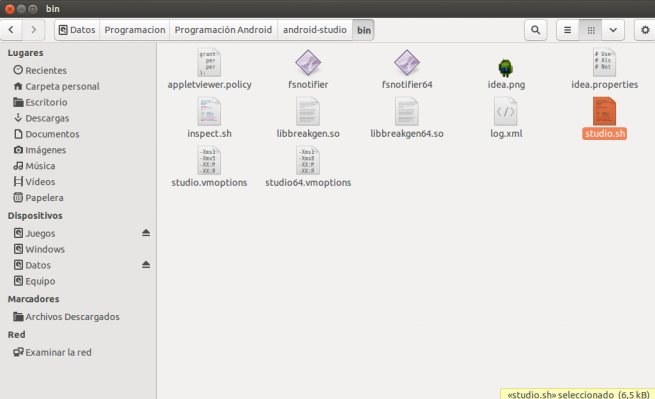
\includegraphics[width=0.6\linewidth]{figuras/and-1}
	\caption{Archivador ubuntu}
	\label{fig:and1}
\end{figure}


Seleccionaremos \textit{New project} para crear un nuevo proyecto desde el que podremos comenzar a utilizar la nueva IDE. Una vez finalizamos el asistente de inicio ya podremos ver la interfaz del programa.

\begin{figure}[H]
	\centering
	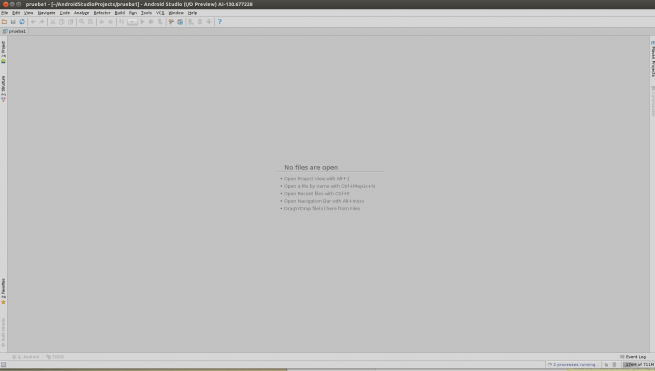
\includegraphics[width=0.7\linewidth]{figuras/and-2}
	\caption{Android studio}
	\label{fig:and2}
\end{figure}

En caso de tener proyectos ya creados o empezados con Eclipse podemos importarlos de forma muy sencilla. Para ello debemos situarnos sobre el \textit{menú file – import} y seleccionar el proyecto que queremos importar. Una vez allí seleccionaremos la opción \textit{Create project from existing sources} y ya tendremos nuestro proyecto importado en nuestro nuevo IDE para continuar desarrollando desde él. Podemos ver que la interfaz de la nueva IDE es bastante simple y sencilla de utilizar.

\begin{figure}[H]
	\centering
	\includegraphics[width=0.7\linewidth]{figuras/and-3}
	\caption{Android studio - ejemplo de proyecto }
	\label{fig:and3}
\end{figure}

\pagebreak

Para crear un lanzador Primero abrimos la consola y digitamos lo siguiente:
\begin{lstlisting}
sudo gedit /usr/share/applications/eclipse.desktop
\end{lstlisting}

Esto obviamente abrirá el gedit y en el ingresamos:

\begin{lstlisting}

[Desktop Entry]
Name=Android Studio
Comment=Android Studio IDE
Exec=/home/tu_usuario/android-studio/bin/studio.sh
Icon=/home/tu_usuario/android-studio/bin/idea.png
Terminal=false
Type=Application

\end{lstlisting}

\subsection{Instalar Xamp}
Descarga el instalador de XAMPP. Puedes conseguirlo en apachefriends.org/download.html. Asegúrate de descargar la versión correcta para tu sistema (32 o 64 bits). En esta guía se utilizará como ejemplo la versión 5.6.3 de 64 bits. Asegúrate de cambiar los comandos según la versión que vayas a instalar.
Abre la Terminal. Antes de poder instalar XAMPP, necesitarás cambiar los permisos de modo que puedas ejecutar el archivo que descargaste. 
Cambia los permisos. Ingresa el siguiente comando y presiona Enter, escribiendo también tu contraseña de ser necesario: 

\begin{lstlisting}

sudo chmod +x xampp-linux-x64-5.6.3-0-installer.run
\end{lstlisting}

Puedes arrastrar el archivo descargado hacia la ventana de la Terminal para ingresar el nombre y la ubicación del archivo en forma automática.
Ejecuta el instalador. Después de cambiar los permisos, podrás ejecutar el instalador para comenzar a instalar XAMPP. Escribe el siguiente comando y presiona Enter: 

\begin{lstlisting}

sudo ./xampp-linux-x64-5.6.3-0-installer.run
\end{lstlisting}

Sigue las instrucciones para instalar XAMPP. Se abrirá el instalador gráfico para guiarte a través del resto del proceso de instalación. En la mayoría de los casos, es mejor dejar todas las opciones con su configuración predeterminada.
\subsection{Instalar Tomcat}
Instalamos Tomcat  en modo terminal.

\begin{lstlisting}

sudo apt-get install tomcat8
\end{lstlisting}

Editamos el archivo de configuración del bash:

\begin{lstlisting}

sudo nano ~/.bashrc
export JAVA_HOME=/usr/lib/jvm/default-java
export CATALINA_HOME=/var/lib/tomcat7
\end{lstlisting}

Por último nos quedaría modificar el archivo de usuarios:

\begin{lstlisting}

sudo nano /var/lib/tomcat7/conf/tomcat-users.xml
Deberemos dejarlo parecido a:
<tomcat-users>
<role rolename="admin-gui"/>
<role rolename="admin-script"/>
<role rolename="manager-gui"/>
<role rolename="manager-status"/>
<role rolename="manager-script"/>
<role rolename="manager-jmx"/>
<user username="admin" password="1234" roles="standard,manager-gui,manager-status,manager-script,manager-jmx,admin-gui,admin-script" />
</tomcat-users>
\end{lstlisting}

Por último, sólo tendríamos que reiniciar el servicio de Tomcat (sudo service tomcat8 restart) y ya podríamos acceder a nuestro Tomcat desde cualquier navegador poniendo la siguiente ruta: localhost:8080 En la que nos aparecerá el archivo por defecto con unos enlaces a los ejemplos, documentación, etc…

Si hemos instalado también el paquete de administración, podremos de una manera sencilla ver, cambiar y desplegar nuestras aplicaciones Java, desde http://local-host: 8080/manager/html introduciendo el usuario y la contraseña que hayamos puesto en el archivo de configuración.


\begin{figure}[H]
	\centering
	\includegraphics[width=0.8\linewidth]{figuras/apache}
	\caption{Tomcat Manager}
	\label{fig:apache}
\end{figure}


\chapter{ANEXO IV}

\section{Configuracion de los proyectos cliente y servidor}

\subsection{Creación del proyecto web service}

Una vez arrancado el entorno Eclipse, vamos a crear un proyecto nuevo (en el menu Archivo -> Nuevo -> Dynamic Web Project.), donde definiremos el nombre de nuestro proyecto, el runtime al que se destina nuestro proyecto, en este caso al servidor tomcat que instalamos en nuestro sistema. Después agregamos al proyecto las librerias de JAX-RS a nuestro proyecto en el boton de “configurar” – “Modificar”.

\begin{figure}[H]
	\centering
	\includegraphics[width=0.4\linewidth]{figuras/service-1}
	\caption{WebService - creación}
	\label{fig:ws1}
\end{figure}

En el directorio src de nuestro proyecto agregamos la siguiente clase “LoggerWS”, dentro del paquete com.group.six:

\begin{lstlisting}[style=JAVA]
package com.intraza.rest;

import javax.ws.rs.Consumes;
import javax.ws.rs.GET;
import javax.ws.rs.POST;
import javax.ws.rs.Path;
import javax.ws.rs.Produces;
import javax.ws.rs.QueryParam;
import javax.ws.rs.core.MediaType;

import org.apache.log4j.Logger;
import org.codehaus.jackson.map.ObjectMapper;

import com.intraza.rest.db.*;
import com.intraza.rest.db.datos.*;

@Path(value = "/sincroniza")
public class InTrazaWS {
	
	private static Logger logger = Logger.getLogger(InTrazaWS.class);
	
	@GET
	@Path("articulos")
	@Produces(MediaType.APPLICATION_JSON)
	public List<Articulo> consultaArticulosBD() {
		return JDBCQuery.getArticulos();
	}
	
	..............
	
	@POST
	@Path("prepedido")
	@Consumes(MediaType.APPLICATION_JSON)
	@Produces(MediaType.APPLICATION_JSON)
	public ResultadoEnvioPedido enviaPrepedidoBD(String jsonPrepedido) {
		ResultadoEnvioPedido resultadoEnvio = null;
		try {
			// Convertimos el JSON que nos llega a un objeto java
			ObjectMapper mapper = new ObjectMapper();
			JsonPedido datosPrepedido = mapper.readValue(jsonPrepedido, JsonPedido.class);
			
			logger.debug("##### observaciones (" + datosPrepedido.getObservaciones() + ") ######");
			
			resultadoEnvio = JDBCQuery.postPrepedido(datosPrepedido);
		} catch (Exception e) {
			resultadoEnvio = new ResultadoEnvioPedido(ResultadoEnvioPedido.CON_ERROR,
			"Se ha producido una excepcion al decodificar JSON (" + jsonPrepedido + ") (" + e.toString() + ")");
		}
		
		return resultadoEnvio;
	}
\end{lstlisting}

Ahora es necesario agregar al archivo web.xml, que eclipse nos genero sobre el directorio WEB-INF de nuestro proyecto, la configuración de Jersey, y el servlet mapping que es la ruta donde se invocara a nuestro servicio, el archivo queda asi:
\begin{lstlisting}[style=JAVA]
<?xml version="1.0" encoding="UTF-8"?>
<web-app xmlns:xsi="http://www.w3.org/2001/XMLSchema-instance"
xmlns="http://java.sun.com/xml/ns/javaee"
xsi:schemaLocation="http://java.sun.com/xml/ns/javaee http://java.sun.com/xml/ns/javaee/web-app_3_0.xsd"
id="WebApp_ID" version="3.0">
<display-name>InTrazaWeb20</display-name>

<servlet>
	<servlet-name>IntrazaWeb</servlet-name>
	<servlet-class>com.sun.jersey.spi.container.servlet. ServletContainer</servlet-class>
	<init-param>
		<param-name>com.sun.jersey.config.property. packages</param-name>
		<param-value>com.intraza.rest</param-value>
	</init-param>
	<init-param>
		<param-name>com.sun.jersey.api.json. POJOMappingFeature</param-name>
		<param-value>true</param-value>
	</init-param>
	<load-on-startup>1</load-on-startup>
</servlet>
<servlet-mapping>
	<servlet-name>IntrazaWeb</servlet-name>
	<url-pattern>/rest/ *</url-pattern>
</servlet-mapping>

<welcome-file-list>
<welcome-file>index.jsp</welcome-file>
</welcome-file-list>
</web-app>
\end{lstlisting}

Para poder compilar y correr nuestro código es necesario antes agregar a nuestro proyecto la implementación Jersey a las librerías de nuestro proyecto, para ello hay que descargarlas del sitio de Jersey, aqui. Para después copiar los jar en el directorio WEB-INF/libs. Otra opción es convertir el proyecto a un proyecto maven, y usar las configuracion a traves del archivo pom.

Para visualizar nuestra aplicación, podemos publicar el servlet al dar Run as -> Run on server. Si aún no tenemos configurado nuestro servidor tomcat, el wizard nos guiara.

La URL donde encontraremos nuestro servicio esta construida de la siguiente manera: http://nuestroservidor:puerto/contextroot/servletmapping/class-path

\begin{itemize}
	\item Nuestroservidor: es el servidor al que publicamos nuestro servlet, con su puerto en el que funciona
	\item Contextroot: es generalmente el nombre de nuestro proyecto, en las propiedades de nuestro proyecto podemos cambiar esto
	\item Servletmapping: es la ruta que definimos en el archivo web.xml donde estaran nuestras clases.
	\item Class-path: es el nombre de la ruta que definimos en nuestra clase con @Path(“/class-path”)
\end{itemize}

\subsection{Integrar un cliente web service}

Por la propia particularidad del web service, un servicio REST, no necesitamos generar un cliente web especifico solo tenemos que tener en cuenta el empaquetado de datos y enviarlos a una url especifica del servicioWeb. Simplemente debemos incluir una clase que gestione la comunicacion. En el codigo siguiente se puede ver un ejemplo que envía al webService un Conjunto de datos a una url especifica.

\begin{lstlisting}[style=JAVA]

package com.six.group.listener.utils;

import android.os.StrictMode;

import com.fasterxml.jackson.databind.ObjectMapper;
import com.six.group.listener.data.json.Datos;

import java.io.BufferedReader;
import java.io.InputStream;
import java.io.InputStreamReader;
import java.io.OutputStream;
import java.net.HttpURLConnection;
import java.net.URL;

public class WebServicesUtils {
private static Integer sincro = 1800;
private static String urlWebServiceRest;


public WebServicesUtils(String puerto, String ip) {
urlWebServiceRest = "http://" + ip + ":" + puerto + "/WebService/enviar/";
}

public String invocaWebServiceHttp(final Datos datos, String action) throws Exception {

StrictMode.ThreadPolicy policy = new StrictMode.ThreadPolicy.Builder()
.detectAll()
.penaltyLog()
.build();
StrictMode.setThreadPolicy(policy);

String result = "";
String urlToInvocate = urlWebServiceRest + action;

System.out.println("Sincronizacion : TRAZA - URL (" + urlToInvocate + ") segundo timeout (" + sincro + ")");

final URL url = new URL(urlToInvocate);
final HttpURLConnection connection = (HttpURLConnection) url.openConnection();
connection.setConnectTimeout(sincro * 1000);
connection.setReadTimeout(sincro * 1000);
connection.setRequestMethod("POST");
connection.setDoOutput(true);
connection.setRequestProperty("Content-Type", "application/json");
final ObjectMapper mapper = new ObjectMapper();
final String jsonRequest = mapper.writeValueAsString(datos);
final OutputStream os = connection.getOutputStream();
os.write(jsonRequest.getBytes());
os.flush();
final InputStream content = connection.getInputStream();
final BufferedReader in = new BufferedReader(new InputStreamReader(content));
String line;
while (null != (line = in.readLine())) {
result += line;
}
return result;
}
}

\end{lstlisting}


\chapter{ANEXO V}

\section{Compilación de los proyectos}

\subsection{Compilación Android}

Lo primero que debemos hacer es abrir nuestro proyecto en Android Studio y asegurarnos de que no hay ningún error de código ni de compilación ya que, de lo contrario, no se completará la compilación.

Si todo está correcto (no tenemos nada marcado en rojo en el código) abriremos el menú \textit{Build} de la parte superior de la pantalla y veremos dos opciones:

\begin{itemize}
	\item Build APK
	\item Generate Signed APK
\end{itemize}	

La primera opción nos va a permitir generar un archivo apk para instalarlo en un dispositivo, pero el archivo no estará firmado. La segunda opción nos permitirá generar un archivo de forma (o utilizar uno existente) para firmar digitalmente nuestra aplicación. Esta opción es para  subir la app al google play.
En nuestro caso vamos a seleccionar directamente la segunda opción, la de generar el archivo APK firmado digitalmente. Pulsamos sobre ella y veremos una nueva ventana similar a la siguiente.

\begin{figure}[H]
	\centering
	\includegraphics[width=0.7\linewidth]{figuras/build-1}
	\caption{Android studio-buid}
	\label{fig:bld1}
\end{figure}


Aquí podemos elegir dos opciones. Si ya tenemos una clave creada anteriormente la cargaremos desde el botón \textit{Choose Existing} e introduciremos el correspondiente nombre, usuario y contraseña para poder utilizarla. 

\begin{figure}[H]
	\centering
	\includegraphics[width=0.6\linewidth]{figuras/build-2}
	\caption{Generar aplicación firmada - key}
	\label{fig:bld2}
\end{figure}

Si nunca hemos generado una clave o queremos crear una nueva por diversos motivos, pulsaremos sobre \textit{Create New}.
Se nos abrirá una nueva ventana como la siguiente:

\begin{figure}[H]
	\centering
	\includegraphics[width=0.6\linewidth]{figuras/build-3}
	\caption{Generar aplicación firmada - nuevo key store}
	\label{fig:bld3}
\end{figure}

En esta ventana debemos rellenar los siguientes apartados:

\begin{itemize}
	\item Key Store Path: Ruta donde guardaremos la clave.
	\item Password: Contraseña 1 para nuestra clave.
	\item Alias: Nombre que daremos a nuestra clave.
	\item Password: Contraseña 2 para nuestra clave.
	\item Validity: Tiendo de validez de la clave (en años).
	\item First and last name: Nombre y apellidos.
	\item Organizational Unit: Nombre de nuestra empresa.
	\item Organization: Nuestra empresa (otra vez)
	\item City: Ciudad.
	\item State: Estado, país.
	\item Country Code: Código de nuestro país.
\end{itemize}


Aceptamos y Android Studio guardará el fichero de la clave en la ruta especificada. Debemos guardar a buen recaudo este archivo ya que sin él perderemos el control sobre nuestra aplicación y no podremos actualizarla más adelante. Una copia de seguridad en un USB y en la nube (cifrada, para evitar robos) es la mejor opción.
Una vez hecho esto, Android Studio cargará automáticamente nuestra clave generada y nos permitirá seguir con la generación del apk.


\begin{figure}[H]
	\centering
	\includegraphics[width=0.6\linewidth]{figuras/build-4}
	\caption{Generar aplicación firmada- key creada}
	\label{fig:bld2}
\end{figure}


Pulsamos \textit{Next} y en el siguiente paso nos preguntará la ruta donde guardará el APK y el tipo de compilación que va a ser (release para publicar o debug para probar y depurar).

Pulsamos sobre Finish y listo. Android Studio compilará nuestra aplicación y la guardará en la ruta especificada. Una vez finalice el proceso veremos un aviso en el IDE que no indica que todas las tareas se han realizado correctamente.

\begin{figure}[H]
	\centering
	\includegraphics[width=0.6\linewidth]{figuras/build-5}
	\caption{Generar aplicacion firmada - finalizar}
	\label{fig:bld2}
\end{figure}

\subsection{Compilación Eclipse}

Para la compilación en eclipse utilizamos Maven. Este ya nos proporciona un WAR generado cuando ejecutamos sus comandos. Pulsamos con el botón derecho sobre el proyecto para elegir “Run As”. En el desplegable podremos comprobar como hay ya varios comandos pre-configurados por el plugin de Maven en Eclipse; es decir, que pulsando un botón ejecutaremos estos comandos sin tener que escribir una palabra en la línea de comandos.

\begin{figure}[H]
	\centering
	\includegraphics[width=0.5\linewidth]{figuras/maven/maven1}
	\caption{Eclipse - opciones maven}
	\label{fig:mvn1}
\end{figure}

\subsubsection{POM}

El archivo descriptivo que contendrá las opciones de compilación, dependencias, etc, es el “pom.xml”, el de resto de pestañas son asistentes para configurar el POM de una manera más sencilla, que aquí no entraremos pero échalas un vistazo que son útiles.

\begin{figure}[H]
	\centering
	\includegraphics[width=0.5\linewidth]{figuras/maven/maven2}
	\caption{Eclipse - pom.xml}
	\label{fig:mvn2}
\end{figure}

Podemos describir su estructura básica con el siguiente listado:

\begin{itemize}
	\item \textbf{build:} Se ocupa de declarar la estructura del proyecto, gestionar plugins, y configura los informes.
	\item \textbf{properties:} Propiedades y/o variables para maven.
	\item \textbf{pluginManagement:} Solo configura los plugins que son referenciados dentro de elementos de los plugins de los hijos (plugins).
	\item \textbf{plugins:} Los plugins nos aportan funcionalidades extra.
	\begin{itemize}
		\item \textbf{groupId,artifactId, version}
		\item \textbf{extensions,inherited, configuration}
		\item \textbf{dependencies} 
	\end{itemize}
	\item \textbf{dependencies:} Son las dependencias (bibliotecas) que sean necesarias para la ejecución de la aplicación.
\end{itemize}

\subsubsection{Run options}

Por mediación del comando “maven install” construiremos un war completamente funcional y desplegable en tomcat. 

\begin{figure}[H]
	\centering
	\includegraphics[width=0.7\linewidth]{figuras/maven/maven3}
	\caption{Eclipse - salida de consola maven}
	\label{fig:mvn3}
\end{figure}
	
	

%----------------------------------------------------------------------------------------

\backmatter

% Bibliografía, glosario, ...
\bibliographystyle{plainnat}
\bibliography{biblio}

\end{document}
%========================================================================================